\documentclass[a4paper,11pt]{article}

%\usepackage[pdftex]{graphicx}
\usepackage{amsmath}
\usepackage[skip=0.5\baselineskip]{caption}
%\usepackage[latin1]{inputenc}
%\usepackage{hyperref}
%\usepackage[T1]{fontenc}
%\usepackage[utf8]{inputenc}
%%GD Quand je mets usepackage[utf8]{inputenc} je n'arrive plus à compiler la biblio
%J'ai essayé de débuger : je n'y suis pas arrivé
\usepackage{rotating}
\usepackage{setspace}
\usepackage{lscape}
\usepackage[round]{natbib}
\usepackage{multirow}
\usepackage{rotating}
\usepackage{vmargin}
\usepackage{epstopdf}
\usepackage{hyperref}
\usepackage{float}
\usepackage{caption}
\usepackage[tableposition=top]{caption}
\usepackage{amsfonts}
\usepackage{bbold}
\usepackage{natbib}
\usepackage{babel,varioref}
\usepackage{bbm}
\usepackage[flushleft]{threeparttable}
%\usepackage{bbold}
%\usepackage[T1]{fontenc}
% JH : impossible de compiler avec le package bbold, remplacé par amsfonts
% LP : impossible de compiler avec le package bbold, remplacé par bbm
\usepackage{upgreek}
\usepackage{comment}
\includecomment{commentGD}
\usepackage[draft]{todonotes}
%\usepackage[disable]{todonotes}
%%GDPour cacher les notes, \usepackage[disable]{todonotes}

\usepackage{setspace}

%\usepackage[nolists, figuresfirst]{endfloat}
%\usepackage{sidefloat}

\setlength{\abovecaptionskip}{-8pt}

%\usepackage[usenames]{color}
%\definecolor{grey}{rgb}{0.35,0.35,0.35}
%\definecolor{webdarkblue}{rgb}{0,0,0.4}
%\definecolor{orange}{rgb}{0.7,0.2,0.05}


%\usepackage[pdfcreator={PDFLaTeX}, pdfproducer={PDFLaTeX}, pdfstartview=FitH, pdfpagemode=UseOutlines, pagebackref=false, colorlinks={true},
%citecolor={webdarkblue}, linkcolor={webdarkblue},
%urlcolor={webdarkblue}]{hyperref}



%\addtolength{\oddsidemargin}{-0.4in}
%\addtolength{\evensidemargin}{-0.4in}
%\addtolength{\textwidth}{0.8in} \addtolength{\topmargin}{-0.85in}
%\addtolength{\textheight}{1.7in}
\renewcommand{\baselinestretch}{1.2}

\newcommand\cites[1]{\citeauthor{#1}'s\ (\citeyear{#1})}

\newcommand\citeh[1]{\citeauthor{#1}'\ (\citeyear{#1})}

\setmarginsrb{3cm}{2cm}{3cm}{2cm}{0,5cm}{0,5cm}{0,3cm}{0,5cm}



% commands

\newcommand{\bi}{\begin{itemize}}
\newcommand{\ei}{\end{itemize}}
\newcommand{\be}{\begin{enumerate}}
\newcommand{\ee}{\end{enumerate}}
\newcommand{\bd}{\begin{description}}
\newcommand{\ed}{\end{description}}
\newcommand{\beqa}{\begin{eqnarray}}
\newcommand{\eeqa}{\end{eqnarray}}
\newcommand{\beq}{\begin{equation}}
\newcommand{\eeq}{\end{equation}}
\newcommand{\bs}{\bigskip}
\newcommand{\A}{$^a$}
\newcommand{\B}{$^b$}
\newcommand{\C}{$^c$}

\renewcommand{\baselinestretch}{1.2}
%\doublespacing

%\linespread{1.6}

%\newcommand{\note}[1]{\footnote{\begin{doublespace}#1\end{doublespace}}}


\begin{document}




\title{\textsc{International Transport costs:\\New Findings from modeling additive costs}\thanks{We thank the referees, as well as the editor, William Kerr, for insightful comments, which helped to significantly improve the paper. We are grateful to Holger G\"{o}rg, S\'{e}bastien Jean and Vincent Vicard for their critics and suggestions on earlier drafts. The paper has also greatly benefited from remarks from the participants at ETSG 17\textsuperscript{th} (Helsinki), DEGIT XXII (Paris), seminars at the universities of California-Irvine, Paris-Dauphine, Paris-I and Nancy and the Kiel Institute for the World Economy. Any remaining errors are ours. This paper was partly funded by a university grant from the University of Lille. It features an online appendix containing additional results, available on the authors' websites.}}

\author{Guillaume \textsc{Daudin}\thanks{%
University Paris-Dauphine \& PSL University, IRD, LEDa, UMR 225, DIAL, 75016 Paris, France; email: \url{guillaume.daudin@dauphine.psl.eu}}  \qquad J\'{e}r\^{o}me \textsc{H\'{e}ricourt} \thanks{Univ. Lille, CNRS, IESEG School of Management, UMR 9221 - LEM - Lille Économie Management, F-59000 Lille, France, and CEPII, France; email: \url{jerome.hericourt@univ-lille.fr}}\qquad Lise \textsc{Patureau}\thanks{Corresponding author.
University Paris-Dauphine \& PSL University, LEDa, 75016 Paris, France;  email: \url{lise.patureau@dauphine.psl.eu} } }


\date{September 2021}
 \maketitle
\bigskip

\begin{abstract}
This paper investigates the pattern of international transport costs over time, using information contained in the US imports flows from 1974 to 2019. First, we document the importance of the per-unit component of transport costs. It represents between one-third and one-half of overall transport costs. Second, allowing for time-varying per-unit costs, we find that the downward trend in international transport costs comes from the reduction in ``pure'' transport costs over time, with trade composition effects playing a minor role. In both aspects, our results point to the importance of the additive component in accounting for international transport costs. \textbf{A REPRENDRE - BIG PICTURE}
\end{abstract}


\thispagestyle{empty} \pagestyle{plain} \setcounter{page}{1}

\bigskip


\noindent \emph{JEL classification}: F10, N70, R40 \\
\noindent \emph{Keywords}: Transport costs estimates, non-linear econometrics, period 1974-2019, additive costs, trade composition effects

{\normalsize \vspace{0cm} }

{\normalsize \titlepage }

{\normalsize \newpage }

%\begin{spacing}{1.5}

\section{Introduction \label{sec:Intro}}


Trade costs are central to international economic analysis. In particular, they are known to be a major obstacle to international economic integration and international trade flows. Defined as the costs associated with the exchange of goods across
national borders, trade costs are usually split between transaction costs, policy costs, time costs and transport costs \textit{per se}. Many argue that the latter have substantially decreased with technological advance in transportation, infrastructure development
and new communication technologies. However, several empirical evidence
suggest that transport costs remain large and deserve attention.\footnote{\cite{anderson_wincoop_jel} find that around 30\% of international trade costs are attributable to transport costs. Equivalently, international transportation costs represent a 21\% markup over production costs. Further, the sizable elasticity of trade with respect to freight costs obtained by \cite{Behar_Venables} (around -3) testifies to the impact of transport costs on trade flows. \cite{Disdier_Head08}, among others, point out that distance as an incompressible cost is still a very important determinant of trade flows.} In addition, progress in transportation techniques (which reduces the constant-dollar cost of transport) should be compared with technical progress in production (which reduces the constant-dollar cost of production) to get a clear picture of the evolution
of the transport costs burden. The latter also depends on whether the cost is in proportion of the value of goods traded (hence does not distort relative prices) or a cost per unit traded (the additive form conversely affecting relative prices). If a complex task, having a clear view of the international transport cost burden is of key importance, since the answers to several important (both academic and policy) economic questions depend in large part on how much distance-based costs affects trade, such as, among others, the dynamics
of agglomeration, the profitability of outsourcing or the gains from trade liberalization. The main contribution of the paper is to bring new insights on this issue.\smallskip


Our paper contributes to the literature by providing a thorough empirical investigation of international transport costs over time based on US imports flows from 1974 to 2019. Importantly, our empirical setting carefully distinguishes between multiplicative and additive transport costs, which proves to be key in the characterization of international trade patterns. While most of the international trade literature has modeled trade costs as an ad-valorem tax equivalent (i.e. as a constant percentage of the producer price per unit traded, part of the ``iceberg cost'' hypothesis in Samuelson's (1954) terminology\cite{samuelson1954}),\footnote{Strictly speaking, the ``iceberg cost'' includes both the ad-valorem dimension of trade cost and the fact that these costs are paid in terms of the good that is traded.
As this last element is irrelevant in our case, we use the terms ``iceberg'' and ``ad-valorem'' interchangeably, as is commonly done in the literature.} a recent strand of the empirical literature points to the existence of an additive component, that is, a cost per unit traded (see, among others, \cite{Irrazabal_2015}, or \cite{martin2012}). Based on US sectoral data, our own estimates also point out the importance of additive costs in international transport costs. Contributing one step further, we provide estimates of the size of both additive and ad-valorem transports costs by sector (at the 3-digit level) and country of origin on a yearly basis over 1974-2019 and by transport mode (air or maritime transport).\smallskip


Our results may be summarized in two main new findings.
First, additive transport costs are quantitatively sizable.
On average over 1974-2019, the additive cost is estimated to be 1.7\% and 2.8\% of the export price in air and vessel transport respectively (at the 3-digit classification level). This is slightly lower than our estimates for the ad-valorem component (2.4\% and 3\% for air/vessel respectively on average over the period).
Put differently, additive costs represent on average between 30 and 45\% of the overall transport costs. To the best of our knowledge, our paper is the first to provide such an extensive quantitative measure of both ad-valorem and additive costs in total transport costs.
This represents a valuable insight for calibrating related international trade or business cycle models.
We also provide an empirical assessment of what standard international trade models lose by skipping additive transport costs.
Quantitatively, the omission of the additive term leads to overestimate the ad-valorem component by a factor around 2. Further, the goodness of fit is systematically better when the additive component is included in the regression, even when taking into account the removed degree of freedom.\smallskip

\textbf{A REPRENDRE - BIG PICTURE EN DEUX POINTS }

Second, we find that the main source of the downward trend in overall transport costs comes mainly from the reduction of transport cost \textit{per se}, by roughly \textbf{50\% in air shipping and 60\% in vessel shipping over 1974-2019}.\footnote{Throughout the paper, we refer to ``pure'' or ``\textit{per se}'' transport costs changes as the changes over time in the transport costs for a given product/country partner, ie excluding trade composition effects (i.e. changes over time in the baskets of imported goods and/or the origin countries).} Specifically, trade composition effects have only limited influence in accounting for the downward trend of international transport costs, and when they matter (in maritime transport), composition effects amplify the reduction of pure transport costs. This contrasts with the conclusion obtained by \cite{hummels2007} yet also on US import flows.%\footnote{Both Hummel's and our's databases come from the US Bureau of Census's import flows database, with two differences yet. First, we consider a larger period of time, spanning from 1974 (as in \cite{hummels2007}) to 2019 (while he stops in 2004). Second, while Hummels considers products at the 5-digit classification level, we are able to exploit heterogeneity in the data at the much more disaggregated HS-10 level for the vast majority of the period (1989-2019). For the period 1974-1988, we rely on Hummel's original database with a 5-digit product classification level.}
\cite{hummels2007} finds that total transport costs have decreased in both air and maritime shipment, but less so than ``pure'' transport costs, because trade composition effects have partly offset the pure transport costs decrease, thereby attenuating the overall downward trend in transport costs. Importantly, we show that the difference of results can be attributed to the new method of modeling the additive component that we offer. Allowing the share of additive costs to vary across time, products and country partners (rather than being constant as in \citealp{hummels2007}), turn out to be key in the decomposition of underlying sources of the decrease of overall transport costs observed over the period.

\smallskip
In both aspects, our results point to the importance of the additive component in accounting for international transport costs.
In this respect, it contributes to the literature that challenges the dominant role of iceberg costs in international trade (even in the case of ice transport, see \citealp{bosker2018ice}). As shown by \cite{alchian}, the relative price of two varieties of some goods will depend on the level of additive trade costs. In this context, the relative demand for more expensive/higher-quality product goods increases with trade costs (``shipping the good apples out''). This is consistent with the empirical findings by \cite{hummels_skiba}, who estimate the elasticity of freight rates with respect to price to be well below unity.\footnote{Also, their estimates imply that doubling freight costs increases average free alongside ship (fas) export prices by 80\% to 141\%, consistent with high-quality goods being sold in markets with high freight costs.}
Recent empirical studies based on micro-level data also provide strong empirical support for the role of additive costs (i.e. cost per unit exported) in international trade costs.\footnote{Based on a firm-product-level database of French exporters, \cite{martin2012} finds that firms charge higher unit values for exports to more remote countries, supporting the importance of additive costs.
Using transaction-level trade data from Colombia, \cite{Lashkaripour-2017} estimates that the transport cost elasticity varies greatly across industries, with a value of 0.8 for the average industry, in contrast with the iceberg specification.} If in empirical support for additive trade costs, these papers yet do not allow for a quantitative measure of these cost (neither for the ad-valorem costs). One important contribution of the paper is to provide quantitative estimates of both type of transport costs.\footnote{On top of the previously cited papers about additive costs, our paper also relates to \cite{Kropf-Saure-JIE-2016}, who estimate the size and shape of per-shipment costs based on Swiss data, and to \cite{Alessandria-et-al-AER-2010} or \cite{Hornok-et-al-JIE-2015, Hornok-et-al-RES-2015}, who point out the role of per-shipment costs (among which, administrative costs) in generating some ``lumpiness'' in international trade transactions.} \smallskip


Closely related to our paper is the work by \cite{Irrazabal_2015}, which develops a structural framework for inferring relative additive trade costs from firm-level trade data.
Implementing their methodology on Norwegian firm-level export data for the year 2004, they find that, for the median shipment, additive costs (in Norwegian crowns) amount to 6\% of the export price multiplied by the ad-valorem cost (also expressed in Norwegian crowns).
Our results share in common with \cite{Irrazabal_2015} the important role of the additive component of international trade costs.
Yet, our paper complements their findings in two main respects.
First, while our study covers a narrower set of trade costs focused on transport costs, their data and their empirical approach only allows the identification of \textbf{the ratio of the additive cost to the export price multiplied by the ad-valorem cost LE DIRE PLUS SIMPLEMENT}; by contrast, our estimation strategy enables us to estimate each value of the ad-valorem and the additive costs independently from the other. From this, we can rebuild the ratio in similar terms to them, thereby gaining in generality in this respect. \textbf{A DEVELOPPER A MINIMA SUR LES IMPLICATIONS EN TERMES DE MODELISATION?}
While \cite{Irrazabal_2015} find that, for an export price multiplied by the ad-valorem cost of 100 USD, 6 USD are paid in additive trade costs, our results point to a value paid in additive transport costs of 2.8 USD for maritime shipping and 1.5 USD for air transport for 2004.
This comparison of results suggests that between a quarter and a half of the additive trade costs are attributable to the transport sector (depending on the transport mode).%JH : these results should not change, they are for 2004.
Second, we exploit exhaustive information about the imports flows of the US over a wide time-span from 1974 to 2019.
In this respect, our results deliver a broader view of the magnitude of additive costs in international trade over time.
In particular, we show that the modeling of additive costs is of critical importance in determining the underlying sources of the trends patterns of international transport costs observed over the last fifty years.

%\textbf{Big Picture}.
Our results are robust to a range of robustness checks, including the use of instrumental variables and more disaggregated data at the SITC 4 or HS10 levels. They have important implications for both international trade and international macroeconomics models. \textbf{Parler des effets de composition comme une des implications}. Beyond the positive aspect, some recent papers also point out the normative implications of additive trade costs. \cite{sorensen2014} thus analytically shows that important welfare gains can be achieved by reducing additive trade costs. Not much progress has yet been made in quantifying such gains, one potential reason being the lack of an empirical characterization of the additive component of trade costs (the one exception being \citealp{Irrazabal_2015}). The quantitative results we provide in the paper allow making one step in filling that gap. %\footnote{ \cite{sorensen2014} extends \cite{melitz}'s seminal model of international trade by including additive trade costs, in addition to the ad-valorem component. A key analytical result is that the welfare gain from a reduction in trade barriers is higher for a decrease in additive costs than a decrease in ad-valorem costs, due to the alteration of relative prices in a heterogeneous-firms trade framework. This is confirmed by \cite{Irrazabal_2015}.}
 %On the same toke, as additive costs distort relative prices, they are very likely to affect the international transmission of shocks in international business cycles models.


More precisely, we use our estimates of multiplicative and additive costs for the years 1974 and 2019 to implement several comparative static exercises investigating the different welfare consequences of alterations to multiplicative and additive costs. For a given decrease in transport costs, welfare gains are around 50\% higher when the underlying framework allows for additive costs - which, in practice, concentrate the major part of transport costs decrease over the period. In addition, we also assess how the latter results are distorted by changes in sunk costs of exports (i.e., increase in the share of exporting firms). Welfare gains are proportionally amplified, with again an additional premium coming from the decrease of additive costs.

%\textbf{To develop}. \medskip

The remainder of the paper is built as follows. The following section presents the data and the baseline empirical model used to estimate the values of international transport costs. Section \ref{sec:basic_results} reports the later on a yearly basis throughout the period 1974-2019 by transport mode, explicitly distinguishing between the additive and the ad-valorem components and providing several important robustness checks of our results. In particular, section \ref{sec:basic_results} reports the mean values of the transport costs estimated over the period (by transport mode). The two following sections take stock of those results to draw implications for two important debates in economic analysis. In section \ref{sec:results_trends}, we offer new insights on the origins of the decrease of transport costs over time, by providing a decomposition of the transport costs trend patterns, between what arises from changes in the trade composition (by product and/or partner country), and what is attributable to changes in transport costs \textit{per se}. Section\ref{sec:theory} implements several theory-based calibration exercises to investigate the different welfare consequences of alterations to multiplicative and additive costs, and section \ref{sec:conclu} concludes.



\section{Estimating international transport costs\label{sec:data_method}}

\subsection{Data}

Our analysis of transportation costs consists of exploiting the difference between commodity-level export and import prices, as in \cite{hummels2007}. The database we use to construct our measure of transport costs comes from the US annual ``Imports of Merchandise'' provided by the US Census Bureau, spanning 1974 to 2019 (details on the database provided in Appendix \ref{app:data}). We first use customs values, quantities and freight costs to recover free alongside ship (fas) and cost-insurance-freight (cif) prices, by good, country of origin and transportation mode.\footnote{The related literature commonly refers to the fob (free on board) price rather than the fas price. The fas price means that the seller must transport the goods all the way to the dock, close enough to be reached by the crane of the ship it will be transported in. It is also the seller's responsibility to clear the goods for export. The fob price means that the seller is obligated to bring the goods all the way to the port, clear the goods for export, and see that they are loaded onto the ship nominated by the buyer. Once the goods clear the railing of the vessel, the buyer assumes the risk. Note that this term is used exclusively for maritime and inland waterway transport. While both terms are closely related, the US Foreign Trade Statistics reports fas prices.} More precisely, the (unit) fas price is computed as the total ``customs value'' in the US trade statistics divided by the shipping weight, both items being conditional to the transport mode; in other words, it is the price for one kg of the goods net of transportation costs, by transport mode.\footnote{One may be concerned by the fact that unit prices are calculated as the value divided by the shipping weight, rather than to the quantity (the number) of goods. This is due to the fact that in the Census data, information on the quantity of goods is not mode-specific. We yet provide a robustness check where unit values are built as the ratio between value and quantity of goods per observation, on a specific sub-sample restricted to US imports flows that only use one single transport mode. \textbf{See Section XXX JH: COULD NOT FIND THESE ANYWHERE. HAS IT BEEN DONE?}. \textbf{LE METTRE EN FOOTNOTE ME PARAIT LEGER, POINT IMPORTANT DU REFERE 1 + bcp de footnotes. Le remonter dans le corps PPL?}} The cif price is then computed as the sum of the customs value and freight charges, once again divided by the shipping weight. Our dependant variable is finally computed as the ratio of the cif price divided by the fas price. By construction higher than 1, the variable provides a measure of transport costs as a proportion of the goods' price, an ad-valorem equivalent. This is quite a standard and widespread strategy, as emphasized by \cite{anderson_wincoop_jel}.

Obviously, this dataset has limitations.
First, it restricts our analysis to the study of international \emph{transport} costs, as our measure of the cif-fas price gap only covers freight, insurance and handling costs.
It is thus silent about the other dimensions of international trade costs.
Second, in terms of transport costs \textit{per se}, our measure omits the ``indirect'' costs related to the time value of goods on their way to their export market (including holding cost for the goods in transit, inventory cost due to buffering the variability of delivery dates, preparation costs associated with shipment size, etc.).
In this respect, this dataset embraces only a partial view of international transport barriers.
However, it is also clear that these direct transport costs do represent a sizable share of trade costs.
According to \cite{anderson_wincoop_jel}, the 21\% markup over production costs coming from transport costs includes both directly measured freight costs (11\%) and ``indirect'' costs that amount to a  9\% tax equivalent.
Further, the evidence summarized in \cite{anderson_wincoop_jel} points to the persisting importance of direct transport costs, especially compared to other trade barriers.
They remain more important than, e.g., policy barriers (8\% tax equivalent), language barrier (7\%) or information cost (6\%).\footnote{In his survey, \cite{Hummels_1999} mentions several papers which all indicate that transport costs pose a barrier similar in size to, or larger than tariffs.
In the same vein, \cite{limao_venables} highlight the importance of infrastructures for trade costs in general, through their impact on transport costs.}

Exploiting this dataset also has three advantages.
First, it comes from a single, homogenous and trustworthy customs source.
This limits the measurement error bias.
Based on customs declarations, the US Imports Database inventories all imports (both values and quantities), by country of origin, to the United States at the HS 10-digit level, with a concordance code to the SITC coding system. In addition, the database reports information regarding freight, insurance and handling expenditures by transportation mode, ocean (or ``vessel'') and air. We will make use of this to highlight potential differences in the magnitude of transport costs across transportation modes.
Second, this dataset provides both the import price and the export price for the same good (for a given origin country).
This is highly valuable, as it gives us a direct measure of international transport costs (at the country/sector level), from which we can estimate separately the levels of both the iceberg costs and of the additive costs, in contrast to e.g. \cite{Irrazabal_2015}.
Third, this dataset is available over a long time span, which enables us to analyze the trend patterns of international transport costs over the period 1974-2019.\footnote{Note that, as mentioned by \cite{Lafourcade_Thisse}, our transport costs measures are based on actual trade flows, i.e. ignoring those flows that did not happen because of presumably prohibitive transport costs.
In light of this, the estimated values that we obtain can be viewed as the lower bounds of the ``potential'' transport costs.} \smallskip


As detailed below, the use of a non-linear estimator triggers computational limitations that limit the level of possible detail, especially when covering a long period of time. This drives us to estimate international transport costs at the 3-digit classification level, exploiting heterogeneity between products at the SITC-5 classification level. Depending on the year, this leaves us with around 200 3-digit sectors, from around 200 countries of origin. We ensure the robustness of these results by conducting two types of alternative estimates: \textit{i,} within each 3-digit sector, exploiting heterogeneity between HS-10 products. Notice that this can be done from 1989 onwards for which HS-10 data are available; \textit{ii,} running the estimation at the 4-digit sector level (still with 5-digit products) for some selected years. The selected years for the 4-digit level estimations are: 1974, 1977, 1981, 1985, 1989, 1993, 1997, 2001, 2005, 2009, 2019. Comparing different levels of aggregation is useful to check differences and the presence of biases precisely due to aggregation. However, we obtain no substantial difference between the results obtained for the benchmark 3-5 sector-product classification levels and those considering either the 3-10 and 4-5 ones (See Appendix \ref{app:4digit}). \textbf{JH: WHERE ARE THE 3-10/4-5 ESTIMATES? NOT IN ANY APPENDICES.}
 \textbf{XXXX-GD:4-5 ESTIMATES are in table 1. 3-10 I am not sure... On y fait allusion dans la procédure en IV, c’est sûr.}



\subsection{Estimating transport costs: empirical specification}

\paragraph{Estimation strategy} Our starting point relates the import price (at the entry gate) of a given good as equal to the export price (at the export gate) plus freight charges. Specifically, denoting by $p$ the price per kg of goods paid by the importer (import, or cif price), $\widetilde{p}$ the (per kg) export (or fas) price and $f$ the shipping charge per kg shipped, we have: $ p = \widetilde{p} +f$. As in \cite{hummels2010}, assume that the shipping charges may depend on the price $\widetilde{p}$ according to the functional form $f = \widetilde{p}^{1-\beta} X$, where $X$ represents all other elements of transport costs (such as distance, port quality, etc.). The link between the import, export prices and shipping charges is hence given by:
%\begin{eqnarray*}
$$ p = \widetilde{p}+f ~~ \Leftrightarrow  ~~ p = \widetilde{p}+\widetilde{p}^{1-\beta} X $$
%\end{eqnarray*}
Defining transport costs $TC \equiv \frac{p-\widetilde{p}}{\widetilde{p}}$, we then obtain:
\begin{equation}
TC \equiv \frac{p-\widetilde{p}}{\widetilde{p}} = \widetilde{p}^{-\beta} X \label{eq:tt1}
\end{equation}
From Equation (\ref{eq:tt1}), it is straightforward that $\beta$ is equal to the elasticity of transport costs to the unit price (in absolute value):

\begin{equation}
\frac{\partial TC}{\partial \widetilde{p}} \frac{\widetilde{p}}{TC} = - \beta \label{eq:alternative}
\end{equation}

From Equation (\ref{eq:tt1}), we can identify a first polar case where $\beta=0$. Shipping charges are proportional to the fas price, such that $p=\widetilde{p}(1+X)$: Only ad-valorem costs apply. At the other extreme, the case $\beta=1$ corresponds to shipping costs being independent of the unit price, with the cif price the sum of the unit price and the shipping cost: Transport costs are fully additive.
This suggests that, the closer $\beta$ to 1, the more prevalent additive costs in total transport costs. One can analytically show that $\beta$ is indeed equal to the share of additive costs in total transport costs.

To do so, start from the link between the link between cif, fas prices and transport costs by explicitly decomposing between the ad-valorem and the additive costs as $p = \tau \widetilde{p}+ t$, with $\tau \geq 1$ the ad-valorem cost and $t>0 $ the additive shipping charge per kg transported. We can rewrite the additive cost as a function of the cost per USD shipped $\widetilde{t} \equiv \frac{t}{\widetilde{p}}$, leading to:
\begin{equation}
p = \tau \widetilde{p}+ \widetilde{t}\widetilde{p}  \label{eq:base}
\end{equation}
Starting from Equation (\ref{eq:base}), the elasticity of transport costs to the unit price $\widetilde{p}$ can be shown to be equal to:\footnote{See \textbf{Appendix XXX for a formal demonstration. XXXJH: WHERE ??? XXX A FIARE?}}
\begin{eqnarray}
\frac{\partial TC}{\partial \widetilde{p}} \frac{\tilde{p}}{TC}&=& \frac{-\frac{t}{\tilde{p}}}{\tau -1  +\frac{t}{\tilde{p}}} \notag \\
&=& -\frac{\widetilde{t}}{\tau-1 +\widetilde{t}} \label{eq:tt2}
\end{eqnarray}

Comparing Equations (\ref{eq:tt1}) and (\ref{eq:tt2}), it is straightforward that the unit price-elasticity of transport costs (in relative terms) is also equal to the share of additive costs in total transport costs.

While many in the related literature provide an indirect measure of additive costs by estimating the elasticity of freight charges to the unit price (\citealp{hummels_skiba}, \citealp{Lashkaripour-2017}), thereby relying on Equation (\ref{eq:alternative}), we propose an alternative route. Based on Equation (\ref{eq:base}), we exploit our dataset to obtain explicit measures of both transport costs components $\tau$ and $t$ (or $\widetilde{t}$). From this, we can deduce the price-elasticity of transport costs as the share of additive costs in total transport costs through Equation (\ref{eq:tt2}).



\paragraph{Obtaining the estimated equation} Let us denote $i$ the origin country, and $k$ the product (at the 5-digit level in our benchmark estimate), for each year-mode specific flow. For sake of reading convenience, we skip the year and transport-mode dimensions in the notations. Transforming the above equation (\ref{eq:base}) as the percentage change in prices induced by transportation, we get the following baseline specification underlying our estimation:

\begin{equation}
\frac{p_{ik}}{\widetilde{p}_{ik}} -1 = \tau_{ik}-1 +\frac{t_{ik}}{ \widetilde{p}_{ik}} \label{eq:base_estimee}
\end{equation}

We follow \cite{Irrazabal_2015} by considering that \textit{i)} both ad-valorem and additive costs are separable between the origin country ($i$) and the product ($k$) dimensions, and \textit{ii)} this separability is in a multiplicative way for the former and an additive way for the latter.
In other words, $\tau_{ik}$ and $t_{ik}$ are written as:\footnote{Notice that, given the magnitude or order of transport costs, assuming an additive or a multiplicative form for country/product fixed effects does not make a substantial difference since, for small values (as we generally obtain), we have $\tau_i\times \tau_k -1\simeq (\tau_i-1) + (\tau_k -1) $ and $t_i+t_k\simeq (1+t_i)\times(1+t_k)-1$.
We also provide a robustness analysis to the separability assumption. Given the much higher number of fixed effects to estimate, we run this robustness check on a sub-sample of goods/origin countries. See Section \ref{sec:robustness} for a detailed presentation of this robustness check.}

\begin{eqnarray}
\tau_{ik} &=& \tau_{i} \times\tau_{k} \label{eq:ad-valorem}\\
t_{ik} &=& t_{i} + t_{k} \label{eq:add}
\end{eqnarray}

\noindent As a result, our underlying structural equation is specified as:

\begin{equation*}
\frac{p_{ik}}{\widetilde{p}_{ik}}-1 =\tau_{i}\times\tau_{k} -1 +\frac{t_{i} + t_{k}}{ \widetilde{p}_{ik}} \label{eq:theory_equation}
\end{equation*}

The ratio $\frac{p_{ik}}{\widetilde{p}_{ik}}$ has a lower bound of one, since by construction, the import price $p$ cannot be lower than the export price ($p_{ik}\geq\widetilde{p}_{ik}$). Taking into account this constraint in the estimate implies that the error term should be always positive.
We ensure that this constraint is fulfilled by specifying the error term as follows:

\begin{equation*}
\frac{p_{ik}}{\widetilde{p}_{ik}}-1 =\left(\tau_{i}\times \tau_{k} -1+\frac{t_{i} + t_{k}}{\widetilde{p}_{ik}} \right)\times \exp(\epsilon_{ik})
\end{equation*}
\noindent where $\epsilon_{ik}$ follows a normal law centered on 0.
Considered in logs, the above equation becomes:

\begin{equation}
\ln\left(\frac{p_{ik}}{\widetilde{p}_{ik}}-1 \right)= \ln \left(\tau_{i}\times \tau_{k} -1+\frac{t_{i} + t_{k}}{\widetilde{p}_{ik}}-1 \right) + \epsilon_{ik} \label{eq:equation0}
\end{equation}

Since Equation (\ref{eq:equation0}) is non-linear, it cannot be estimated using standard linear estimators. All estimates are thus performed using non-linear least squares.\footnote{The basis of the method is to approximate the model by a linear one and to refine the parameters by successive iterations. The intuitive criterion for convergence is that the sum of squares of residuals does not increase from one iteration to the next.
See \cite{Woolridge-Book-2001} for more details.} Yet, the use of a non-linear estimator triggers computational limitations that limit the level of possible detail, especially when covering a long period of time.
Confronted with this trade-off, we estimate international transport costs at the 3-digit level as our benchmark classification, even though data series are available at a more disaggregated product level ($k=5$ in our benchmark estimates). This amounts to making the additional assumption, that all 5-digit products $k$ in a 3-digit sector $s$ share the same structure of costs.\footnote{One way to gauge the relevance of this assumption is to provide a decomposition variance exercise on the observed cif-fas price.
As reported in Appendix \ref{app:decomp_variance}, the share of the observed variance that is accounted for by the between-sectors ($s$) variance is roughly similar to the between-product ($k$) variance.}$^{,}$\footnote{One may object that we could preserve the estimation at the 5-digit level by running an OLS estimation on the equation taken in level, i.e.
on the basis of Equation (\ref{eq:base_estimee}), specifying the error term additively.
This would not solve the problem though, for three main complementary reasons.
First, at the 5-digit level the number of fixed effects to include in the estimation would be more than 430,000 (with 216 countries and 2,029 products), making the estimation computationally extremely burdensome, even in OLS.
Imposing Equations (\ref{eq:ad-valorem}) and (\ref{eq:add}) to reduce the number of fixed effects would drive us back to the non-linearity issue for fixed effects.
Second, making the error term (specified as following a normal law centered on 0) enter Equation (\ref{eq:base_estimee}) additively implies negative values for some of the estimated residuals $\widehat{\epsilon}_{ik}$, which is inconsistent with the constraint that $\frac{p_{ik}}{\widetilde{p}_{ik}}>1$.
Third, estimating the equation in level does not eliminate the fact that it is non-linear by nature, as long as there are additive costs to estimate (see Equation (\ref{eq:base_estimee}) for $t_{ik} \neq 0$).}

This drives us to estimate a modified version of Equation (\ref{eq:equation0}), specified as:
\begin{equation}
\ln\left(\frac{p_{ik}}{\widetilde{p}_{ik}}-1 \right)= \ln \left(\tau_{i}\times \tau_{s(k)} -1+\frac{t_{i} + t_{s(k)}}{\widetilde{p}_{ik}} \right) + \epsilon_{ik} \label{eq:model_IetA}
\end{equation}
where $\tau_{i}$, $\tau_{s(k)}$, $t_{i}$ and $t_{s(k)}$ are the parameters to be estimated, i.e., fixed effects specific to each origin country $i$ and sector $s$ (at the 3-digit classification level), and $\epsilon_{ik}$ the residual centered on 0.\footnote{Note that, strictly speaking, the exact equation that we estimate is the following:
$$\ln\left(\frac{p_{ik}}{\widetilde{p}_{ik}}-1 \right)= \ln \left(\sum_i \alpha_i^\tau \mathbbm{1}_i \times \sum_{s(k)}\alpha_{s(k)}^\tau \mathbbm{1}_{s(k)}-1 + \frac{\sum_i\alpha_i^t\mathbbm{1}_i + \sum_{s(k)}\alpha^t_{s(k)}\mathbbm{1}_{s(k)}}{\widetilde{p}_{ik}}\right)+\epsilon_{ik} $$
After proceeding to the estimation, we uncover the estimated values of the transport costs components $\tau_{i}$, $\tau_{s(k)}$, $t_{i}$, $t_{s(k)}$ from the obtained coefficients $\alpha^{x}_{z}$ for $x=\tau,t$ and $z=i,s(k)$ (by year and transport mode).
For reading convenience, we adopt a lighter expression of this equation by resorting to the notations of $\tau_i,\tau_{s(k)}$ and $t_i$, $t_{s(k)}$ as a short-cut.}  To eliminate the potential influence of outliers, we exclude 5\% of the upper and lower tails of the distribution in the regression variables.
%JH: TO KEEP IN MIND: one day, we could be asked to winsorize tails, instead of cutting them...
These cut-offs are aimed at eliminating reporting or coding errors.
We estimate Equation (\ref{eq:model_IetA}) for each year over the period 1974-2019, for each of the transportation modes reported (air or vessel), on a sectoral-origin country basis ($i,s$).
Depending on the year considered, this leaves us with around 800 fixed effects to estimate by transport mode at the 3-digit level.
  \medskip



As mentioned in the Introduction, one contribution of the paper is to provide a careful estimation of international transport costs, which decomposes into both an additive and an ad-valorem component.
In this respect, our paper relates to the recent literature about the importance of additive costs in accounting for international trade costs (\citealp{Irrazabal_2015}, among others).
We contribute to this issue by adopting the following strategy.
For each year and transport mode, we estimate two models.
In Model (a), additive costs are excluded, transport costs being modeled as iceberg costs only. In this case, the estimated equation simplifies as:

\begin{equation}
\ln\left(\frac{p_{ik}}{\widetilde{p}_{ik}}-1 \right)= \ln \left(\tau_{i}\times\tau_{s(k)}-1 \right) + \epsilon^{ice}_{ik} \label{eq:model_nlI}
\end{equation}

Under Model (b), transport costs are decomposed in the two additive and ad-valorem dimensions (Equation (\ref{eq:model_IetA})).
From this, we compare the fitting properties and the explanatory power of both models to evaluate the importance of modeling the additive component.\footnote{One may object that a comprehensive study of the structure of transport costs should also include the third model with only additive costs. This has driven us to estimate this third model (c) as well, in which case the estimated equation is written according to: $\ln\left(\frac{p_{ik}}{\widetilde{p}_{ik}}-1 \right)= \ln \left(\frac{t_{i} + t_{s(k)}}{\widetilde{p}_{ik}}\right) + \epsilon^{add}_{ik}$.
The main result that emerges is that this model (c) is dominated (in terms of quality of fit properties) by the model (a) with multiplicative costs only, which is itself dominated by the complete model (b), anticipating further results. More details of these results are given in the Online Appendix.}


%One may be concerned that the specification of Equations (\ref{eq:model_IetA}) or (\ref{eq:model_nlI}) might be subject to an endogeneity bias, as the price set by the exporter may vary depending on the transport cost burden.
%Studies on the pricing-to-market behavior of firms (see \citealp{Krugman-87}) show that we cannot exclude that the export price set by the firm ($\widetilde{p}_{ik}$) is partly endogenous to the size of transport costs (for instance, the exporting firm absorbing (part of) the transport costs by reducing the fas price).
%This is not an issue here, as we are not interested in causal inference.
%Rather, our aim is to provide an accounting breakdown of transport costs between the additive and the multiplicative components.

%However, we consider as a reasonable assumption that the exporting firm cannot influence the international transport cost sector, that would imply a causal effect of the firm's prices on the transport costs value, except in the choice between air and vessel transport (that is beyond our scope of analysis).
%Otherwise stated, conditional to an export price and a transport mode, the gap between the export price declared to the custom data and the import price recorded by the US administration is beyond the firm's control.
%In this respect, we are confident that our estimation strategy is immune from endogeneity problems.

%\textbf{pas encore completement clair. Veut-on dire que ce qui est pbtique, c'est que TC reagisse a ptilde? Je crois que ce qu'on veut dire, c'est que le fait que ptilde change en fonction des TC ne change pas les TC, le cif price s'ajuste proportionnellement? Si c'est ca, c'est vrai seulement si les couts sont advalorem...Pour dire que les firmes peuvent difficilement influencer le prix du transport au niveau 3d, on pourrait donner des stats des la dessus? Par produit 3d/pays, par secteur 3d tous pays, etc...?}\smallskip


After estimating Equation (\ref{eq:model_IetA}), we can rebuild a measure of each component, $\widehat{\tau}^{adv}_{is(k)} = \widehat{\tau_{i}} \times \widehat{\tau}_{s(k)}$ for the ad-valorem cost and $\widehat{t}_{is(k)} = \widehat{t}_{i} + \widehat{t}_{s(k)}$ for the additive cost, that are country-sector specific, by year and transport mode.
When assuming iceberg costs only (Equation (\ref{eq:model_nlI})), we proceed similarly to get $\widehat{\tau}^{ice}_{is(k)} = \widehat{\tau}_{i} \times \widehat{\tau}_{s(k)}$.
In this case, notice that the equation could be estimated relying on a linear form.
To preserve comparability of the results, we keep the same non-linear estimation method in both cases.
Similarly, as \cite{Irrazabal_2015}, we take the average over the sector-country dimension, using the values of each trade flow ($is$-specific) over total yearly trade as a weighting scheme.
We thus recover a ``synthetic estimate'' of each type of transport cost: $\widehat{\tau}^{ice}$ for Model (a), $\widehat{\tau}^{adv}$ and $\widehat{t}$ for Model (b), for each year and transportation mode.
These results are reported in Section \ref{sec:results_decomposition}.


\section{Transport costs: Quantifying their size and structure}\label{sec:basic_results}

\textbf{In this section, we... INTRODUIRE CE QU'ON FAIT}

\subsection{The importance of the additive component \label{sec:results_decomposition}}

%Our ambition to re-assess the underlying sources of the trend patterns of international transport costs requires a careful modeling of both the additive and the multiplicative components.
\paragraph{Quantification} The first step of the analysis consists of providing a quantification of the magnitude of transport costs over time (by transport mode), distinguishing whether the additive component $t_{ik}$ is excluded or included in the estimated equation (Equation (\ref{eq:model_IetA}) or (\ref{eq:model_nlI})).
This allows us to provide estimates for the size of both the ad-valorem and the additive components of transport costs, and assess whether additive costs represent a sizable component of the latter.
These results constitute our first original contribution to the literature.
\smallskip

\begin{table}[htbp]
 \centering
\caption{Transport costs estimates: summary} \vspace{5mm} \label{tab:summary_results}
	\begin{tabular}{lllll}
\cline{1-5}
\multicolumn{1}{c}{} &
  \multicolumn{2}{|c}{3-digit} &
  \multicolumn{2}{c}{4-digit} \\
\multicolumn{1}{c}{} &
  \multicolumn{1}{|r}{air} &
  \multicolumn{1}{r}{ves} &
  \multicolumn{1}{r}{air} &
  \multicolumn{1}{r}{ves} \\
\cline{1-5}
\multicolumn{1}{l}{\textbf{Data}} &
  \multicolumn{1}{|r}{} &
  \multicolumn{1}{r}{} &
  \multicolumn{1}{r}{} &
  \multicolumn{1}{r}{} \\
\multicolumn{1}{l}{\hspace{1em}{$\#$ obs.}} &
  \multicolumn{1}{|r}{16,118} &
  \multicolumn{1}{r}{19,007} &
  \multicolumn{1}{r}{44,331} &
  \multicolumn{1}{r}{41,773} \\
\multicolumn{1}{l}{\hspace{1em}{$\#$ sectors}} &
  \multicolumn{1}{|r}{204} &
  \multicolumn{1}{r}{239} &
  \multicolumn{1}{r}{637} &
  \multicolumn{1}{r}{707} \\
\multicolumn{1}{l}{\hspace{1em}{$\#$ origin countries}} &
  \multicolumn{1}{|r}{169} &
  \multicolumn{1}{r}{164} &
  \multicolumn{1}{r}{213} &
  \multicolumn{1}{r}{212} \\
\multicolumn{1}{l}{\hspace{1em}{\textit{Obs. transport costs $(p/\widehat{p}-1)$ (in $\%$)}}} &
  \multicolumn{1}{|r}{} &
  \multicolumn{1}{r}{} &
  \multicolumn{1}{r}{} &
  \multicolumn{1}{r}{} \\
\multicolumn{1}{l}{\hspace{2em}Mean} &
  \multicolumn{1}{|r}{17.4} &
  \multicolumn{1}{r}{11.4} &
  \multicolumn{1}{r}{3.7} &
  \multicolumn{1}{r}{5.4} \\
\multicolumn{1}{l}{\hspace{2em}Median} &
  \multicolumn{1}{|r}{10.5} &
  \multicolumn{1}{r}{8.3} &
  \multicolumn{1}{r}{1.7} &
  \multicolumn{1}{r}{4.1} \\
\multicolumn{1}{l}{\hspace{2em}Std. dev.} &
  \multicolumn{1}{|r}{23.8} &
  \multicolumn{1}{r}{14.8} &
  \multicolumn{1}{r}{6.0} &
  \multicolumn{1}{r}{5.0} \\
\multicolumn{1}{l}{\hspace{1em}{\textit{Obs. transport costs (USD per kg)}}} &
  \multicolumn{1}{|r}{} &
  \multicolumn{1}{r}{} &
  \multicolumn{1}{r}{} &
  \multicolumn{1}{r}{} \\
\multicolumn{1}{l}{\hspace{2em}Mean} &
  \multicolumn{1}{|r}{2.0} &
  \multicolumn{1}{r}{0.4} &
  \multicolumn{1}{r}{58.4} &
  \multicolumn{1}{r}{0.2} \\
\multicolumn{1}{l}{\hspace{2em}Median} &
  \multicolumn{1}{|r}{0.8} &
  \multicolumn{1}{r}{0.1} &
  \multicolumn{1}{r}{2.8} &
  \multicolumn{1}{r}{0.1} \\
\multicolumn{1}{l}{\hspace{2em}Std. dev.} &
  \multicolumn{1}{|r}{19.0} &
  \multicolumn{1}{r}{10.3} &
  \multicolumn{1}{r}{613.9} &
  \multicolumn{1}{r}{2.5} \\
\multicolumn{1}{l}{{\textbf{Model (A)}}} &
  \multicolumn{1}{|r}{} &
  \multicolumn{1}{r}{} &
  \multicolumn{1}{r}{} &
  \multicolumn{1}{r}{} \\
\multicolumn{1}{l}{\hspace{1em}{\textit{Multiplicative term (in $\%$)} ($\widehat{\tau}^{ice}$)}} &
  \multicolumn{1}{|r}{} &
  \multicolumn{1}{r}{} &
  \multicolumn{1}{r}{} &
  \multicolumn{1}{r}{} \\
\multicolumn{1}{l}{\hspace{2em}Mean} &
  \multicolumn{1}{|r}{6.5} &
  \multicolumn{1}{r}{8.1} &
  \multicolumn{1}{r}{3.5} &
  \multicolumn{1}{r}{4.7} \\
\multicolumn{1}{l}{\hspace{2em}Median} &
  \multicolumn{1}{|r}{5.7} &
  \multicolumn{1}{r}{7.2} &
  \multicolumn{1}{r}{2.5} &
  \multicolumn{1}{r}{3.9} \\
\multicolumn{1}{l}{\hspace{2em}Std. dev.} &
  \multicolumn{1}{|r}{5.1} &
  \multicolumn{1}{r}{4.6} &
  \multicolumn{1}{r}{3.5} &
  \multicolumn{1}{r}{3.0} \\
\multicolumn{1}{l}{{\textbf{Model (B)}}} &
  \multicolumn{1}{|r}{} &
  \multicolumn{1}{r}{} &
  \multicolumn{1}{r}{} &
  \multicolumn{1}{r}{} \\
\multicolumn{1}{l}{\hspace{1em}{\textit{Multiplicative term (in $\%$)} ($\widehat{\tau}^{adv}$)}} &
  \multicolumn{1}{|r}{} &
  \multicolumn{1}{r}{} &
  \multicolumn{1}{r}{} &
  \multicolumn{1}{r}{} \\
\multicolumn{1}{l}{\hspace{2em}Mean} &
  \multicolumn{1}{|r}{6.7} &
  \multicolumn{1}{r}{6.1} &
  \multicolumn{1}{r}{2.2} &
  \multicolumn{1}{r}{3.1} \\
\multicolumn{1}{l}{\hspace{2em}Median} &
  \multicolumn{1}{|r}{5.7} &
  \multicolumn{1}{r}{5.3} &
  \multicolumn{1}{r}{1.5} &
  \multicolumn{1}{r}{2.5} \\
\multicolumn{1}{l}{\hspace{2em}Std. dev.} &
  \multicolumn{1}{|r}{5.0} &
  \multicolumn{1}{r}{3.8} &
  \multicolumn{1}{r}{2.6} &
  \multicolumn{1}{r}{2.7} \\
\multicolumn{1}{l}{\hspace{1em}$\widehat{\beta}$:  \textit{Share of additive costs}} &
  \multicolumn{1}{|r}{} &
  \multicolumn{1}{r}{} &
  \multicolumn{1}{r}{} &
  \multicolumn{1}{r}{} \\
\multicolumn{1}{l}{\hspace{2em}Mean} &
  \multicolumn{1}{|r}{-0.40} &
  \multicolumn{1}{r}{-0.32} &
  \multicolumn{1}{r}{-0.34} &
  \multicolumn{1}{r}{-0.42} \\
\multicolumn{1}{l}{\hspace{2em}Median} &
  \multicolumn{1}{|r}{-0.37} &
  \multicolumn{1}{r}{-0.27} &
  \multicolumn{1}{r}{-0.31} &
  \multicolumn{1}{r}{-0.40} \\
\multicolumn{1}{l}{\hspace{2em}Std. dev.} &
  \multicolumn{1}{|r}{0.27} &
  \multicolumn{1}{r}{0.23} &
  \multicolumn{1}{r}{0.23} &
  \multicolumn{1}{r}{0.27} \\
\cline{1-5}
\end{tabular}

		\begin{tablenotes}
		\tiny
		\item Statistics are obtained weighting each observation by its value relative to total trade flows.
		\item 1989 trade by air is excluded
		%\item The additive term is expressed in fraction of fas price.
		\item For the  4-digit model, statistics for observed data have been calculated for the same set of years as used for estimation, i.e.
		1974, 1981, 1989, 2001, 2009, 2013, 2017 and 2019
		\item \textbf{Model (a): With ad-valorem transport costs only}
		\item \textbf{Model (b): With additive and ad-valorem transport costs}
	\end{tablenotes}
\end{table}

Table \ref{tab:summary_results} reports a summary of our results.
It displays the weighted mean and median values of each type of transport costs (either ad-valorem estimated alone or estimated along with additive costs), as well as the associated standard deviation, averaged over the period 1974-2019, for estimation driven both at the 3- and 4-digit sectorial level for different specifications and data.\footnote{In Appendix \ref{app:more_results}, we report similar results for a sample of years, for both transport modes, at the 3- and 4-digit classification level. Results for all years (available at the 3-digit level) are reported in the Online Appendix, available on the authors' webpages.}
The top panel reports the same set of descriptive statistics, but for the actual cif/fas ratio in our data. In the medium panel, we report the results for a specification based on ad-valorem costs estimated alone (Model (a), based on Equation (\ref{eq:model_nlI})). The bottom panel presents our estimates for a specification involving both ad-valorem and multiplicative components (Model (b), based on Equation (\ref{eq:model_IetA})).

%\begin{table}[htbp]
 % \centering
 % \footnotesize{
 % \caption{Transport costs estimates: summary \label{tab:summary_results}}
 % \begin{center}
  %  \begin{tabular}{l|cc|cc}
  %    \hline \hline
  %  \multicolumn{5}{c}{Mean value over 1974-2013}   \\
  %  \# digit & \multicolumn{2}{c}{3 digits} & \multicolumn{2}{c}{4 digits} \\ \hline
   % Mode  & Vessel & Air ($^{\ast \ast}$) & Vessel & Air \\ \hline
   % \multicolumn{5}{l}{\textbf{Model (a) - With only Ad-Valorem Transport Costs} ($\widehat{\tau}^{ice} -1$, in \%)}  \\ \hline
  %  Mean  & 5.8 & 5.1 & 6.0 & 4.9 \\
  %  Median & 5.1 & 4.2 & 5.2 & 3.7 \\ \hline
    %Std   & 0.032 & 0.042 & 0.036 & 0.045 \\
    %Min.
%value & 1.003 & 1.001 & 1.003 & 1.000 \\
    %Max.
%value & 1.304 & 1.685 & 1.408 & 2.051 \\ \hline
 %   \multicolumn{5}{l}{\textbf{Model (b) - With Additive \& Ad-Valorem Transport Costs} } \\ \hline
 %  \textit{Ad-valorem term ($\widehat{\tau}^{adv}-1$, in \%)} & & & & \\ \hline
 %   Mean  & 3.2 & 2.5 & 3.3 & 2.4 \\
  %  Median & 2.8 & 1.8 & 2.8 & 1.6 \\ \hline
    %Std   & 0.023 & 0.023 & 0.025 & 0.026 \\
    %Min.
%value & 1.001 & 1.000 & 1.000 & 1.000 \\
    %Max.
%value & 1.227 & 1.474 & 1.264 & 1.537 \\ \hline
  %  \textit{Additive term }& & & &   \\ \hline
  %  \textit{In \% of the export price ($\widehat{t}/\widetilde{p}$, in \%)} &&&& \\ \hline
  %      Mean  & 2.9 & 1.8 & 2.8 & 1.9 \\
  %  Median & 1.9 & 0.7 & 1.7 & 0.8 \\ \hline
 %  \textit{In USD per kg traded ($\widehat{t}$)}&&&& \\ \hline
  %  Mean & 0.09	&1.12	&0.08&	2.16 \\
  %  Median & 0.07	&1.04	&0.06&	1.06 \\ \hline
    %Std   & 0.041 & 0.034 & 0.039 & 0.034 \\
    %Min.
%value & 0.000 & 0.000 & 0.000 & 0.000 \\
    %Max.
%value & 2.941 & 13.303 & 3.197 & 11.440 \\ \hline
  %  \multicolumn{5}{l}{\textbf{Data}  } \\ \hline
   % Transport costs ($p/\widetilde{p} -1$, in \%) & & & & \\ \hline
   % Mean & 5.3 & 5.0& 5.6&3.9 \\
   % Median & 4.3 & 2.0 & 4.4& 1.9 \\ \hline
    %Export price ($\widetilde{p}$), in USD & & & & \\
    %Mean & 16.0 &	6488.4	&9.6	&6643.6 \\
    %Median & 4.1	& 142.5	& 4.1	& 142.2 \\ \hline
    %\# obs.
%& 29279 & 28207 & 29317 & 27680 \\
%    \# origin country & 188 & 191 & 188 & 189 \\
%    \# products & 230 & 211 & 666 & 567 \\  \hline \hline
%  \end{tabular}
 %   \end{center}}
%\parbox[l]{12cm}{\footnotesize{Notes: Statistics are obtained weighting each observation by its value relative to total trade flows.
%The additive term is expressed in fraction of fas price.
%For the  4-digit classification, statistics for observed data have been calculated for the same set of years as used for estimation, i.e. 1974, 1981, 1989, 2001, 2009, 2013. ($^{\ast \ast}$): 1989 omitted in 3-digit estimation for air.}}
%\end{table}%

Before jumping to the interpretation, Table \ref{tab:summary_results} calls for two comments of statistical order. First, the estimated mean values are systematically higher than medians. This result is not surprising though, given that our key variable is by nature bounded to 0; therefore, outliers can only be positive, pushing the mean upward compared to the median. Second, the estimated total costs are not exactly equal to the observed ones, in particular for Model (a). This might be accounted for by recalling that all our estimates are based on log-linearization. Therefore, what matters on the statistical ground is that the mean of our predicted values (based on logarithms) must be equal to the mean of the log-linearized data ($\ln\left(\frac{p_{ik}}{\widetilde{p}_{ik}}-1 \right)$), which does not necessarily imply equality between values.
Descriptive statistics showing that both observed and predicted values do match in logarithms are available upon request to the authors.

%One can also note that estimated total costs are most of the time higher than observed costs by 0.5 to 1 percentage point.
%This is first due to the fact that observed data are \textit{de facto} trade-weighted (i.e. by the weight of each good in total trade) while our estimates are based on simple arithmetic means within sector and country.



\paragraph{Interpretation} Coming now to interpretation, two main results emerge from Table \ref{tab:summary_results}.
First, it provides estimation results about the size of the overall transport costs.
Table \ref{tab:summary_results} shows that transport costs amount to around a 5.5-6\% markup in ocean shipping, and 4\% markup in air shipping on average over 1974-2019.\footnote{Expressed as a markup over production costs, transport costs are equal to $\frac{p-\widetilde{p}}{\widetilde{p}}$.
Under Model (a) (ad-valorem costs only), this gives a markup of 5.5\% in vessel, and 4.8\% in air shipping (considering the mean value over the period).
Under Model (b), total transport costs are equal to $\frac{p-\widetilde{p}}{\widetilde{p}} = (\tau-1) + \frac{t}{\widetilde{p}}$.
With $\tau= 1.030$ and $\frac{t}{\widetilde{p}}= 0.028$ in vessel (as reported in Table \ref{tab:summary_results}), we get a value equal to 5.8\%.
A similar calculus gives 4.1\% in air transport.} If this seems modest in comparison with the 11\% of markup obtained by \cite{anderson_wincoop_jel} over a set of industrialized countries, it stands in line with the results obtained by \cite{hummels2007} for the US economy.\footnote{Beyond country coverage and time period, another plausible explanation for the difference with \cite{anderson_wincoop_jel}, lays in the difference of empirical methodology.
\cite{anderson_wincoop_jel}'s estimates are based on standard gravity equations, while ours come from a non-linear estimation of a ``structural'' decomposition of the difference between export and import prices.}

Second, and most importantly, Table \ref{tab:summary_results} provides new quantitative evidence about the size of the additive component of transportation costs.
On average over the whole period, for sectors defined at the 3-digit level, additive costs amount to around 10 cents (0.1 USD) per kilogram exported in maritime transport, and 1.13 USD per kilogram exported in air transport, indicating that freight rates are much higher in the latter case.
Expressed in terms of the export price, the additive costs amount to 2.8\% and 1.7\% for ocean shipping and air transport respectively.
This is slightly lower than the estimates for the ad-valorem component, which is estimated at 3\% and 2.4\% for vessel and air shipping respectively (on average over the period).
Put differently, the additive component amounts to 44\% of total transport costs in vessel, and 30\% in Air, as displayed in the last rows of Table \ref{tab:summary_results}: The per-kg cost dimension is quantitatively sizable.
\medskip

We also provide diagnostic tests about the goodness-of-fit measures, which confirm the empirical relevance of adding the additive component in the estimation. Appendix \ref{app:diagnostic_test} reports quality-of-fit diagnostic tests that confirm the importance of the additive cost component.
The goodness of fit is systematically better when the additive component is included in the regression, even when taking into account the removed degree of freedom. For both transport modes, the omission of the additive term seriously biases the ad-valorem term upward, by roughly a factor 2.\smallskip


Our estimation results on the size of additive transport costs can be compared to \cite{Irrazabal_2015}, the most recent evidence on this question.
Based on Norwegian trade data for 2004, \cite{Irrazabal_2015} estimate that additive costs (in Norwegian crowns) amount to 6\% of export price multiplied by the ad-valorem cost (expressed in Norwegian crowns), i.e.
$\frac{t}{\tau\widetilde{p}}=6\%$ expressed in our terminology (with $\tau>1$, and retaining their estimated weighted mean value, which is the one directly comparable to our own results).
One important difference with respect to their work is that we can provide separate estimates for each cost component (additive and ad-valorem).
From this, we can rebuild the ratio in similar terms to them, allowing us to gain in generality in this respect.
Making use of our estimates for 2004 (see Tables \ref{tab:result_air_3d_detail} and \ref{tab:result_ves_3d_detail} in Appendix \ref{app:more_results}), we thus obtain a ratio $\frac{t}{\tau\widetilde{p}}=2.8\%$ in ocean shipping and 1.5\% in air transport.
This may seem surprisingly low, in contrast to the 6\% obtained by \cite{Irrazabal_2015}.
This can be accounted for by recalling the difference in the type of dataset - hence, of costs, embraced in each case.
While the database of \cite{Irrazabal_2015} allows studying trade costs in general, our database covers a subset made of the monetary international transport costs, as we start from the gap between the import and the export prices (on top of differences due to the country coverage of the two databases).
In this respect, our two papers can be used in a complementary fashion to infer the proportion of additive trade costs that are due to international shipment.
\cite{Irrazabal_2015}'s results on the year 2004 imply that, for an export price multiplied by the ad-valorem cost of 100 USD, 6 USD are paid in additive trade costs.
For the same export price multiplied by the ad-valorem cost of 100 USD, our results for 2004 yield the value of 2.8 (1.5) USD paid in additive transport costs for maritime (air) transport.\footnote{Also notice that, in both papers, starting from the estimated value of the ratio $\frac{t}{\tau \widetilde{p}}= x$, we can rebuild the proportion of additive costs in terms of the import price $\frac{t}{\tau \widetilde{p} + t} = \frac{x}{1+x}$.
Given our estimates for 2004 ($x = 0.028$ and $0.015$ in vessel and air transport respectively), we get a ratio $\frac{t}{\tau \widetilde{p} + t}$ equal to 2.7\% and 1.4\% in each transport mode respectively.} This comparison of results suggests that between 25\% (air) and 47\% (vessel) of additive trade costs are attributable to international transport.
On top of our results summarized in Table \ref{tab:summary_results}, this points to evidence that the additive component represents a quantitative sizable dimension of international transport costs.\smallskip


\subsection{A first look at the time dynamics of transport costs}

In this section, we investigate the trend patterns of international transport costs over time, by exploiting the time dimension of our database.
This focus is shared with some of the international trade literature, such as \cite{Lafourcade_Thisse}, \cite{hummels2007} and \cite{Behar_Venables}. Along with the pattern of total transport costs over time, our empirical set-up also allows us to investigate whether additive costs we put forward so far looking at the average, is a long-lasting, i.e. a structural phenomenon.

\paragraph{Total transport costs: A first look at the trend patterns} Figure \ref{fig:Trends_in_TC} displays the evolution of total transport costs over the period, summing the additive and the ad-valorem estimated costs expressed in percentage of the fas price,\footnote{Specifically, we use the yearly values of the estimated transport cost components averaged over the country/product dimensions (at the 3-digit level), corresponding to the numbers reported for each year in detail in the Online Appendix.
Each yearly value is obtained as: $\widehat{\tau}-1+\frac{\widehat{t}}{\widetilde{p}}$.} by transport mode for each year between 1974 and 2019.

\begin{figure}[htbp]
\caption{Trend in estimated transport costs (yearly mean value)}
\label{fig:Trends_in_TC}
\begin{center}
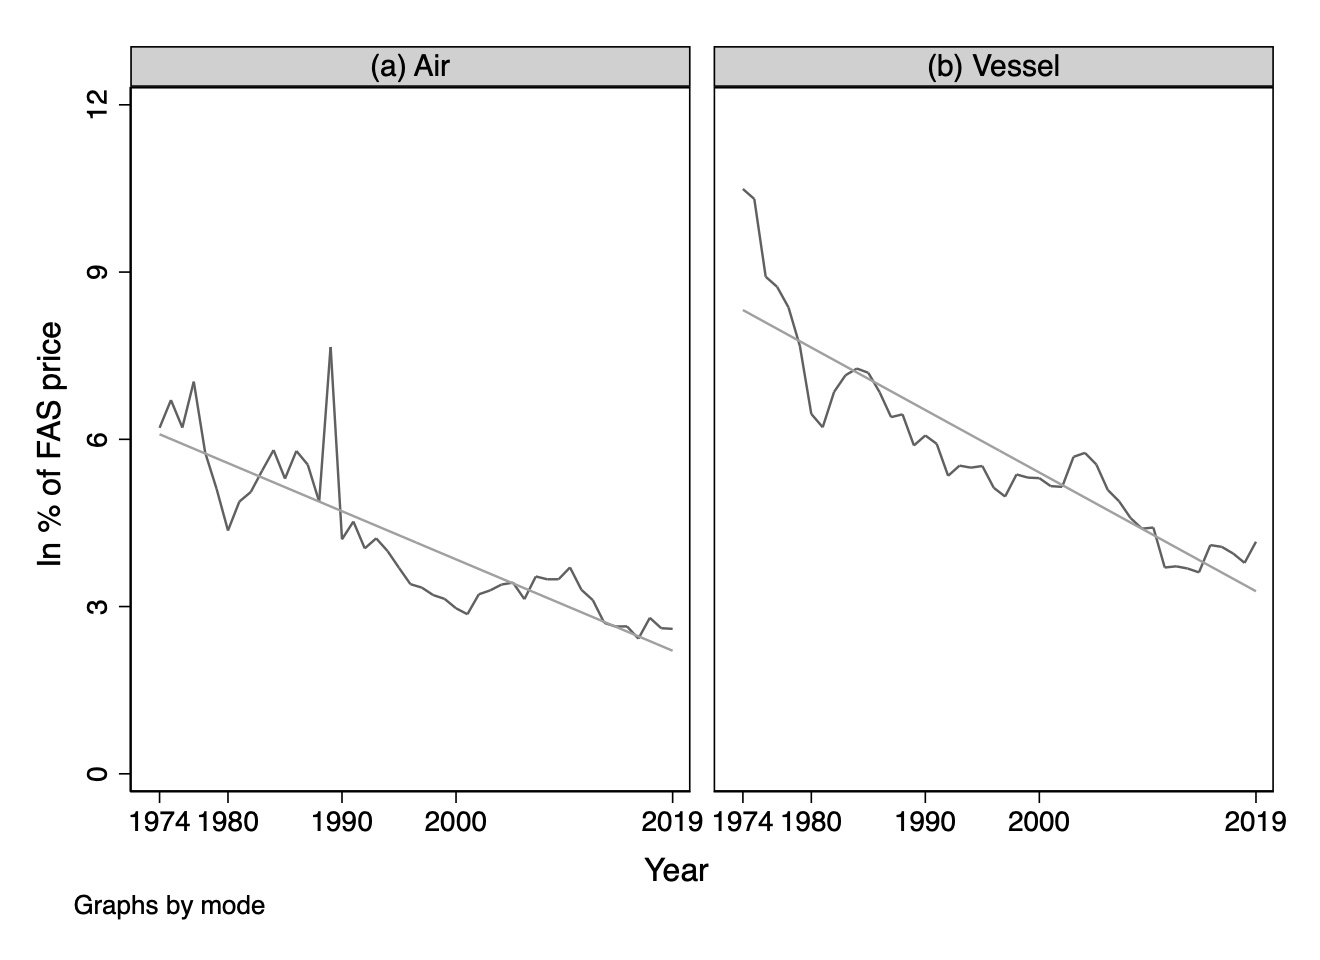
\includegraphics[width=14cm, height=7cm]{Figure2_Trend_of_totalTC_bymode.jpg}
\end{center}
\end{figure}

As shown in Figure \ref{fig:Trends_in_TC}, both air and vessel shipping exhibit a downward trend in overall transport costs since 1974, by \textbf{ACTUALISER LES CHIFFRES -2.1\% per year for mean air transport costs and -2.0\% per year XXX JH à GD : STP, refaire tourner la regression sous-jacente} for mean vessel transport costs, implying a 50\% decrease in air and a 60\% decrease in vessel over the period.\footnote{One may be puzzled by the high magnitude of estimates for the beginning of the period (until 1980 approximately) for vessel transport.
\cite{hummels2007} finds similar outcomes on tramp prices indexes, and suggests the oil shock as a likely culprit, in a context where technological progress was quicker in aviation than in vessel, allowing a better dampening of oil shocks on air freight rates.
In a related manner, one may worry that the strong decrease in transport costs documented in Figure \ref{fig:Trends_in_TC} springs from high oil-shock-related transport costs in 1974. However, computing the time trends from 1980 does not dramatically change the picture.
The yearly trend from 1980 is -2\% for mean air transport costs and -1.6\% for mean vessel transport costs.
We thus choose to exploit the whole time dimension of our database by taking 1974 as starting date of our time-trend analysis.} Using US data, \cite{Hummels_1999} found that overall transport cost declined from 6\% to 4\% of the import value between 1974 and 1996.
For the same years, we obtain a total decrease from 6.9\% to 4.2\% in terms of the export price, on average for air shipping, and from 9.8\% to 4.8\% for ocean shipping. Overall, our results display trends confirm and extend those reported by \cite{Hummels_1999} up to the very recent years.\smallskip

\paragraph{The share of additive costs: Time dynamics} As next step, we investigate whether additive costs are a long-lasting, i.e. a structural phenomenon.

We investigate this point by reporting the share of additive costs in total transport costs on a yearly basis, in both air and vessel transport, based on the weighted-mean values $\widehat{t}/\widetilde{p}$ and $\widehat{\tau}$ (in similar terms as those reported in Tables \ref{tab:result_air_3d_detail} and \ref{tab:result_ves_3d_detail}.
The corresponding values reported in detailed tables are available in section B of the Online Appendix), as displayed in Figure \ref{fig:part_cout_additif}.
Each yearly value is obtained as: $\frac{\frac{\widehat{t}}{\widetilde{p}}}{\widehat{\tau}-1+\frac{\widehat{t}}{\widetilde{p}}}$, expressed in percent of the export price $\widetilde{p}$ (at the 3-digit level).

\begin{figure}[htbp]
\caption{Share of additive costs (3-digit classification)}
\label{fig:part_cout_additif}
\begin{center}
 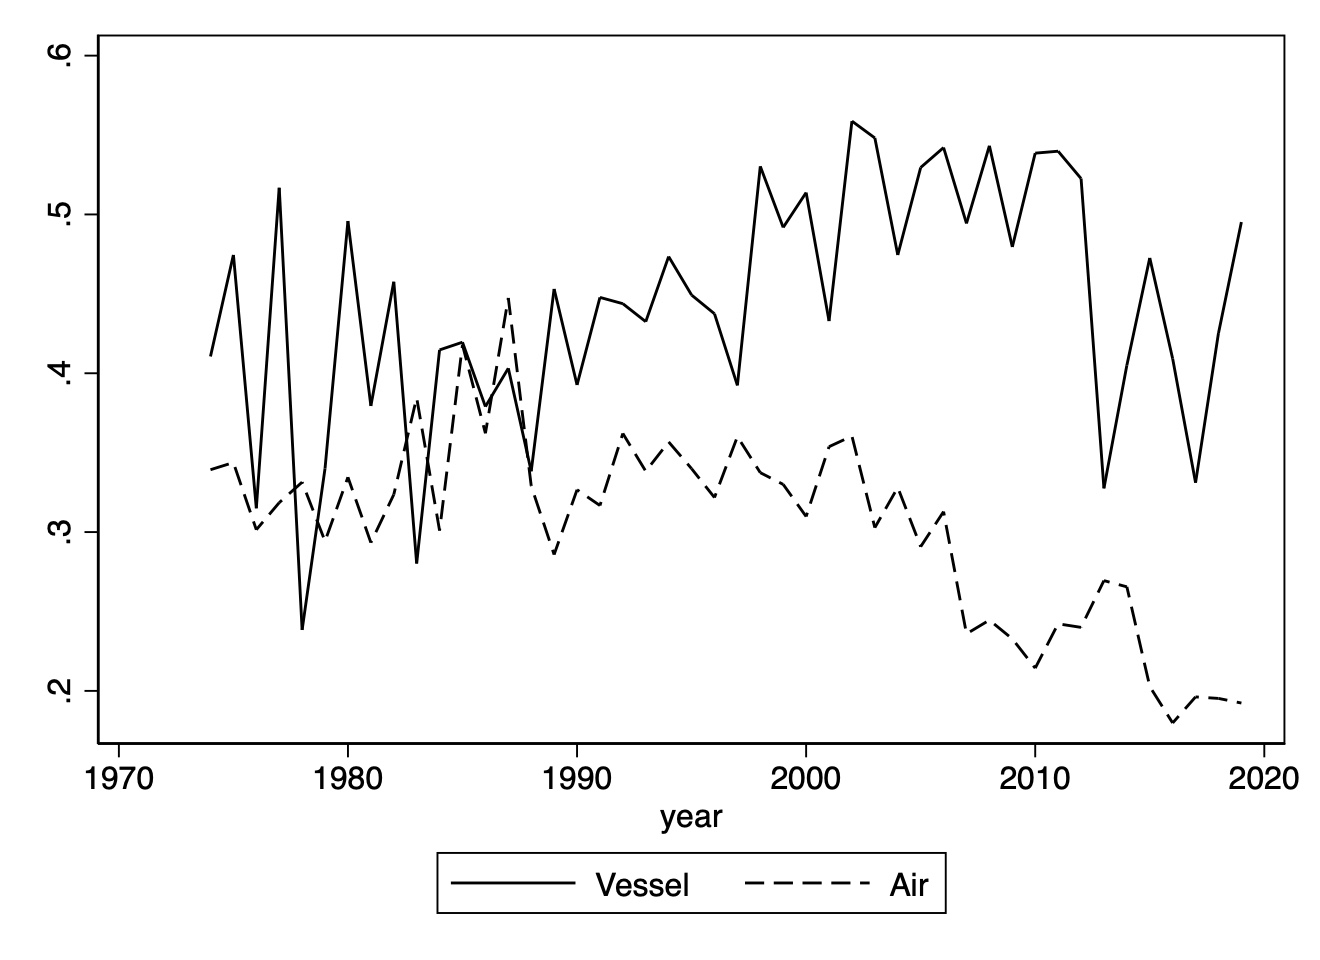
\includegraphics[width=12cm, height=7.5cm]{Figure1_share_of_additive_in_totalTC.jpg}
%{\footnotesize {OECD data} }
\end{center}
\end{figure}


In both transport modes, the additive component appears of sizable importance throughout the period.
Confirming the results obtained in Table \ref{tab:summary_results}, this suggests that additive costs are neither negligible in magnitude nor an erratic phenomenon.
On the contrary, they represent a sizable and structural dimension of international transport costs.
If the share of additive costs in total costs roughly amounts to 44\% (30\%) in vessel (air) transport on average, one can further notice that it varies substantially over time, with a different pattern across transport modes. In maritime transport, the share of additive costs fluctuates around the average, while it has been steeply declining since the end of the 1980s in air transport.

\paragraph{Wrap-up} Our results so far show that total transport costs have strongly reduced between 1974 and 2019, especially in ocean transport. Further, if additive costs represent a substantial share of total transport costs considered on average over the period for both transport modes, a yearly-based inspection reveals marked fluctuations in the share of additive costs in total costs over time. In air transport specifically, the share of additive costs has been declining over time since the beginning of the 1990s. This suggests that the transport costs decrease is more than proportionally due to additive costs in air transport, but more equally shared between ad-valorem and additive costs in ocean transport.

In the following section, we check the robustness of these results regarding two important issues, the separability assumption of country-good fixed effects and potential endogeneity biases.

\subsection{Robustness analysis \label{sec:robustness}}


\subsubsection{Robustness to the separability assumption}
In this section, we provide a robustness analysis to the separability assumption of country-good fixed effects, which considers (following \citealp{Irrazabal_2015}) that both the ad-valorem and the additive costs are separable between the origin country ($i$) and the product ($s(k)$) dimensions.
That is, we relax Equations (\ref{eq:ad-valorem}) and (\ref{eq:add}) to model $\tau_{is(k)}$ and $t_{is(k)}$ (on a yearly/transport mode basis).
Yet, this comes at the cost of having to estimate a much larger number of fixed effects (for approx. 200 countries of origin and 200 sectors at the 3-digit level, this means estimating 40,000 versus 400 fixed effects, per year and per transport mode), making the estimation (all the more given our non-linear setting) intractable in practice.
This drives us to conduct the analysis on a sub-sample of trade flows, upon which two estimations are conducted (for every year and each transport mode): with the separability assumption (Equations (\ref{eq:ad-valorem}) and (\ref{eq:add}) hold, our baseline case) and without.
For each year and transport mode, we select the countries ($i$) and the products (at the 3-digit level, $s(k)$) that constitute 80\% of the total value of trade flows. Table \ref{tab:robustness_separability} shows a summary of the results, considering the average estimated values over the period (by transport mode).
%
%\begin{table}[htbp]
%  \centering
%  \caption{Robustness to the separability assumption (average over the period) - restricted sample}
%\begin{center}
%    \begin{tabular}{lcc|cc}
%    \hline \hline
%    \multicolumn{5}{c}{Mean value over 1974-2019} \\
% \multicolumn{5}{c}{3 digits} \\    \hline \hline
%   Mode  & \multicolumn{2}{c|}{Air} & \multicolumn{2}{c}{Vessel} \\ \hline
%   Separability & No  & Yes (baseline) & No & Yes (baseline)\\ \hline
%    \multicolumn{5}{l}{\textit{Additive term} ($\widehat{t}/\widetilde{p}$.
%in \%)}  \\
%    Mean  & 1.76 & 1.96 & 2.61 & 2.99 \\
%    Median &0.65 & 0.84 &1.83 & 2.23 \\ \hline
%    \multicolumn{5}{l}{\textit{Ad-valorem term} ($\widehat{\tau}$, in \%)}\\
%    Mean  & 1.04 & 0.94 & 2.43 & 2.40 \\
%    Median & 0.56 & 0.83 & 2.06 & 2.04 \\ \hline
%\multicolumn{5}{l}{\textit{Share of additive costs in total costs (in \%)}} \\
%    Mean  & 62.8  & 67.5  & 51.8  & 55.4 \\
%    Median & 54.1  & 50.5  & 47.0  & 52.2 \\  \hline
% \textit{Diagnostic test} & & &  &  \\
%    %$R^2$    & \multicolumn{1}{c}{0.80} & \multicolumn{1}{c}{0.68} & \multicolumn{1}{c}{0.67} & \multicolumn{1}{c}{0.45} \\
%    %SER   & \multicolumn{1}{c}{0.57} & \multicolumn{1}{c}{0.72} & \multicolumn{1}{c}{0.53} & \multicolumn{1}{c}{0.69} \\
%    AIC criteria & 4657.60 & 4654.23 & 10744.83 & 10690.80 \\ \hline
%    %Log-likelihood & \multicolumn{1}{c}{-1757.75} & \multicolumn{1}{c}{-2258.24} & \multicolumn{1}{c}{-4018.51} & \multicolumn{1}{c}{-5220.00} \\ \hline
%\# observations & 2381 & 2381 & 2798 & 2798 \\
%\# origin country & 13.4 & 13.4 & 19.8 & 19.8 \\
%\# products & 25.5 & 25.5 & 53 & 53 \\ \hline \hline
%    \end{tabular}%
%\end{center}
%\parbox[l]{12cm}{\footnotesize{Notes: Estimations are performed on a restricted sample, based on the following rule: for each year and transport mode, we select the countries ($i$) and the products (at the 3-digit level, $s(k)$) that constitute 80\% of the total value of trade flows.
%The additive term is expressed in fraction of fas price. 1989 omitted in 3-digit estimation for air.}}
%\label{tab:robustness_separability}
%\end{table}

\begin{table}[htbp]
	\centering
	\caption{Robustness to the separability assumption - restricted sample}
	\begin{center}
			\begin{tabular}{l|cccc}
\cline{1-5}
\multicolumn{1}{l}{Transport mode} &
  \multicolumn{2}{|c}{Air} &
  \multicolumn{2}{|c}{Vessel} \\
\cline{1-5}
\multicolumn{5}{l}{\textbf{Data}} \\ \hline
%\multicolumn{5}{l}{\hspace{1em}Mean}  \\
\multicolumn{1}{l|}{\hspace{2em}{$\#$ obs.}} &
  \multicolumn{2}{c|}{2,125} &
  \multicolumn{2}{c}{5,260} \\
\multicolumn{1}{l|}{\hspace{2em}{$\#$ sectors}} &
  \multicolumn{2}{c|}{25} &
  \multicolumn{2}{c}{54}  \\
\multicolumn{1}{l|}{\hspace{2em}{$\#$ origin countries}} &
  \multicolumn{2}{c|}{14} &
  \multicolumn{2}{c}{20} \\ \hline
  \multicolumn{5}{l}{{\textbf{Estimations}}}  \\ \hline
  \multicolumn{1}{l}{Separability} &
  \multicolumn{1}{|c}{Yes (Baseline)} &
  \multicolumn{1}{c}{No} &
  \multicolumn{1}{|c}{Yes (Baseline)} &
  \multicolumn{1}{c}{No} \\ \hline
\multicolumn{5}{l}{\hspace{1em}{\textit{Multiplicative term, in $\%$} ($\widehat{\tau}^{adv}-1$)}}  \\ \hline
\multicolumn{1}{l}{\hspace{2em}Mean} &
  \multicolumn{1}{|c}{0.9} &
  \multicolumn{1}{c}{1.0} &
  \multicolumn{1}{|c}{2.3} &
  \multicolumn{1}{c}{2.3} \\
\multicolumn{1}{l}{\hspace{2em}Median} &
  \multicolumn{1}{|c}{0.7} &
  \multicolumn{1}{c}{0.5} &
  \multicolumn{1}{|c}{1.7} &
  \multicolumn{1}{c}{1.9} \\ \hline
\multicolumn{5}{l}{\hspace{1em}{\textit{Additive term, in $\%$} ($\widehat{t}/\widetilde{p}$)}}  \\ \hline
\multicolumn{1}{l}{\hspace{2em}Mean} &
  \multicolumn{1}{|c}{1.8} &
  \multicolumn{1}{c}{1.6} &
  \multicolumn{1}{|c}{2.9} &
  \multicolumn{1}{c}{2.5} \\
\multicolumn{1}{l}{\hspace{2em}Median} &
  \multicolumn{1}{|c}{0.7} &
  \multicolumn{1}{c}{0.6} &
  \multicolumn{1}{|c}{2.1} &
  \multicolumn{1}{c}{1.7} \\ \hline
\multicolumn{5}{l}{\hspace{1em}$\widehat{\beta}$:  \textit{Share of additive costs}}  \\ \hline
\multicolumn{1}{l}{\hspace{2em}Mean} &
  \multicolumn{1}{|c}{0.48} &
  \multicolumn{1}{c}{0.52} &
  \multicolumn{1}{c}{0.55} &
  \multicolumn{1}{c}{0.49} \\
\multicolumn{1}{l}{\hspace{2em}Median} &
  \multicolumn{1}{|c}{0.51} &
  \multicolumn{1}{c}{0.55} &
  \multicolumn{1}{|c}{0.58} &
  \multicolumn{1}{c}{0.48} \\ \hline
\multicolumn{1}{l}{\hspace{1em}AIC} &
%\multicolumn{1}{l}{\hspace{1em}Mean} &
  \multicolumn{1}{|c}{4,841} &
  \multicolumn{1}{c}{4,857} &
  \multicolumn{1}{|c}{12,053} &
  \multicolumn{1}{c}{12,154} \\
\cline{1-5}
\end{tabular}

	\end{center}
	\parbox[l]{12cm}{\footnotesize{Notes: Estimations are performed on a restricted sample, based on the following rule: for each year and transport mode, we select the countries ($i$) and the products (at the 3-digit level, $s(k)$) that constitute 80\% of the total value of trade flows.
			The additive term is expressed in fraction of fas price.}}
	\label{tab:robustness_separability}
\end{table}

Three main comments can be made. First, the subset of large trade flows we are considering (around 8\% of the observations of our initial sample, but 80\% of the total value of aggregated trade) involve a higher share of additive costs: between 52\% and 67\% of total costs on average, versus 40\% to 50\% on the whole sample.
%JH: la phrase suivante est en contradiction avec celle qui suit encore juste après: "Second, assuming that country/product fixed effects are separable in these two dimensions tends to overestimate the value and the share of the additive costs."
Second, both models provide a similar quality of fit of the regression (once we take into account the number of right-hand-side variables) as the AIC criteria display very close values in both models (conditional on transport mode).
Third, the estimated values remain of similar magnitude under both separability and non-separability assumptions, even if one can note that under the separability assumption, the share of additive costs seems slightly biased upward, at least for averages over the period. The picture is reversed for medians.


Before jumping to the conclusion that our results are robust to the separability assumption, however we investigate this comparison deeper on a year-to-year basis, as shown in Figure \ref{fig:robustesse_non_separe}. Specifically, Figure \ref{fig:robustesse_non_separe} displays the results for air transport in panel (a) and for maritime transport in panel (b). In each case, the estimated values (as well as the fitted regression line) under both separability (baseline) and non-separability are reported, for the additive term (upper panel) and the ad-valorem term (lower panel).


\begin{figure}[htbp]
\caption{Robustness to the separability assumption (year-to-year basis)}
\label{fig:robustesse_non_separe}
\begin{center}
\begin{tabular}{cc}
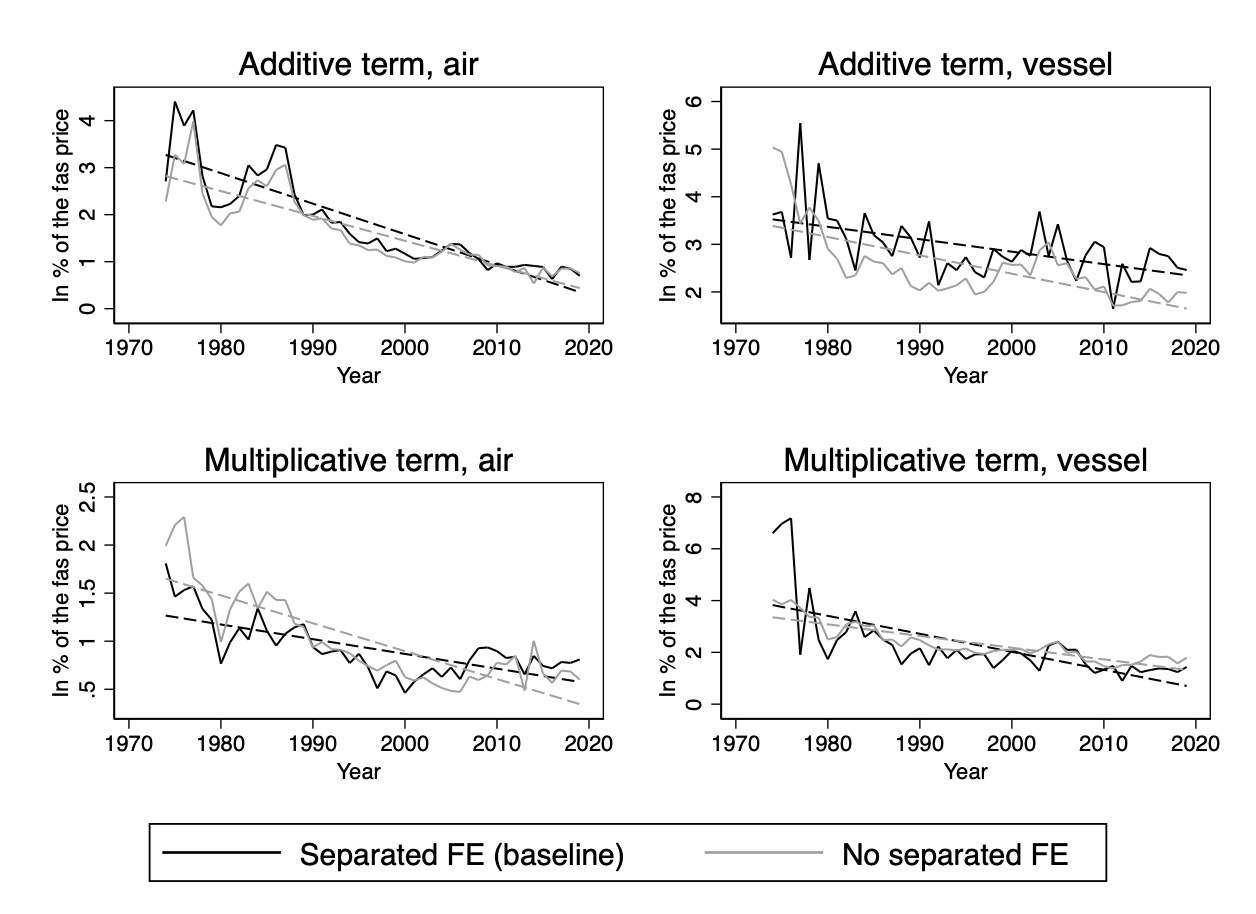
\includegraphics[width=6in, height=4in]{graph_robustesse_ns.jpg}

\end{tabular}
\end{center}
\begin{minipage} [c]  {5in} \scriptsize%
Notes: FE for (country, sector) fixed effects.
\end{minipage}
\end{figure}

In line with Table \ref{tab:robustness_separability}, the results shown in Figure \ref{fig:robustesse_non_separe} confirm that the separability assumption (retained in our baseline estimation) tends to overestimate the value of the additive cost component (and underestimate the value of the ad-valorem cost).
However, they also show that the difference is quantitatively small. Further, and most importantly, whatever the transport mode and for both types of transport costs, the trend patterns of international transport costs, whether estimated under the separability assumption or not, are very similar. Along with the quality-of-fit diagnosis, this confirms the robustness of our estimation results to this assumption.

As an ultimate check, we investigate whether the varying pattern over time/country of origin/product pointed out in Section \ref{sec:results_decomposition} is also robust to the separability assumption. With this aim, Figure \ref{fig:histogram_beta_robustness} shows the histogram of the distribution of the elasticity of transport costs to the export price ($\beta_{ikt}$, for air transport (top panel) and for maritime transport (bottom panel) under the baseline specification (Panels (a), (c))) and the non-separability scenario (Panels (b), (c)).


\begin{figure}[htbp]
\caption{Histogram of the share of additive costs in total costs (restricted sample)}
\label{fig:histogram_beta_robustness}
\begin{center}
\begin{tabular}{cc}
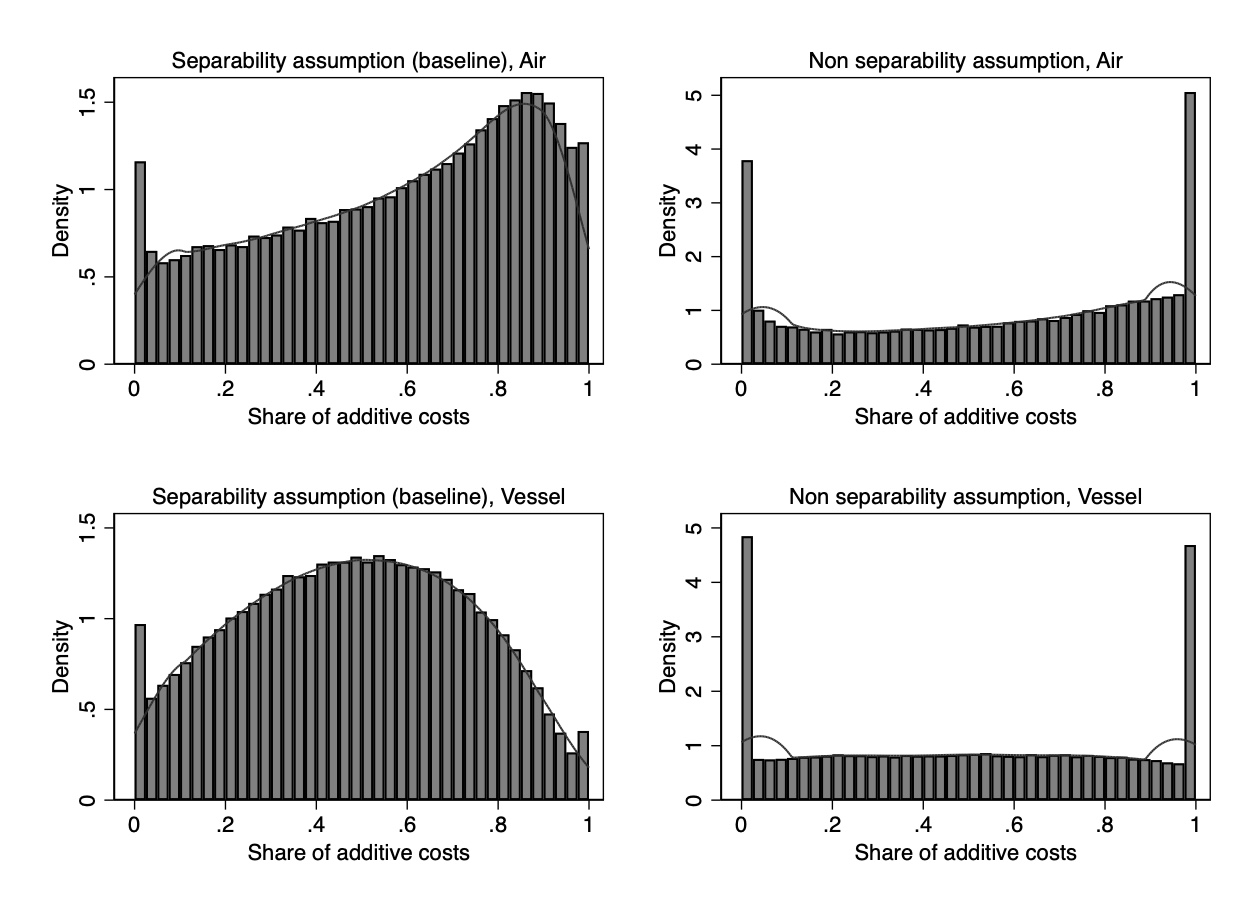
\includegraphics[width=14cm, height=10cm]{Etude_beta_pond.jpg}\\
\multicolumn{2}{l}{{\footnotesize Notes: Distribution of $\beta_{ikt}$ over the triplet (year-product-country), weighted by share of yearly value of flow.}}\\
\end{tabular}
\end{center}
\end{figure}

For both transport modes the distribution of $\beta_{ikt}$ over the triplet (year, country of origin, product) appears smoothly distributed over the interval $[0,1]$, whatever the assumption regarding the specification of fixed effects.
Relaxing the assumption that fixed effects are separable between the two country and product dimensions does not alter qualitatively our conclusion, that the elasticity of transport costs to the export price (or the share of additive costs in total transport costs), is strongly varying over time, countries of origin and products.
\footnote{As a consequence, this also provides an indirect robustness check to the results regarding the trend decomposition provided in Section \ref{sec:results_trends}, which establish that the decline of ``pure'' transport costs is a main reason for the decrease of overall transport costs observed over time.}


\subsubsection{Endogeneity concerns} One may be concerned that the specification of Equations (\ref{eq:model_IetA}) or (\ref{eq:model_nlI}) might be subject to an endogeneity bias, as the price set by the exporter may vary depending on the transport cost burden. Studies on the pricing-to-market behavior of firms (see \citealp{Krugman-87}) show that we cannot exclude that the export price set by the firm ($\widetilde{p}_{ik}$) is partly endogenous to the size of transport costs (for instance, the exporting firm absorbing (part of) the transport costs by reducing the fas price).
Besides, related concerns may arise from productivity-sorting model in \cite{melitz} or the quality-sorting model in \cite{baldwin_harrigan}: more productive firms and/or firms selling high-quality products will charge higher prices, all other things equal – in our case, for a given country-product pair. In addition, there is also the possibility that bigger firms might impact transport costs, due to their ability of bargaining discounts for larger shipped volumes.

It is true we are not interested in causal inference, since our aim is to provide an accounting breakdown of transport costs between the additive and the multiplicative components. However, the latter can be biased by the aforementioned endogeneity issues since they imply that $\frac{1}{\widetilde{p}_{ik}}$ is correlated in one direction on another with residuals $\epsilon_{ik}$. This may ultimately harm the estimation of $\widehat{t}/\widetilde{p}$ and consequently, $\widehat{\tau}$.

Therefore, we propose to compare our main estimates with those stemming from a two-stage least-squares procedure. Put differently, we follow earlier literature (see e.g. \citealp{Caliendo_Parro_2015} or \citealp{Lashkaripour-2017}) by replacing in the right-hand side of Equation (\ref{eq:model_IetA}) $\widetilde{p}$ by predicted values stemming from a first-stage equation regressing $\widetilde{p}$ on custom duties coming based on tariffs at the product line, together with one-year lagged fas prices. Section \ref{app:first_stage_IV} in Appendix \ref{app:more_results} provides a full presentation of the theoretical basis for the first-stage equation, as well as first-stage estimates. In particular, it shows that our main instrumental variable displays the right statistical properties, and that we can confidently re-inject the predictions arising from the first-stage equation for $\widetilde{p}_{ik}$ on the right-hand side of Equation (\ref{eq:model_IetA}\footnote{Note that, since the predictions are expressed in logarithms, they are transformed through the exponential function before their implementation in Equation (\ref{eq:model_IetA}.} to produce a 2SLS-type of estimation. Figure \ref{fig:comp_IV_SITC5} below reports our benchmark estimates by transport mode, together with their instrumented counterpart. In all cases, these estimates are very similar, when not identical. This supports that our benchmark estimates do not suffer any substantial biases arising from endogeneity concerns.

\begin{figure}[htbp]
\caption{Transport cost time trends: robustness to IV procedure}
\label{fig:comp_IV_SITC5}
\begin{center}
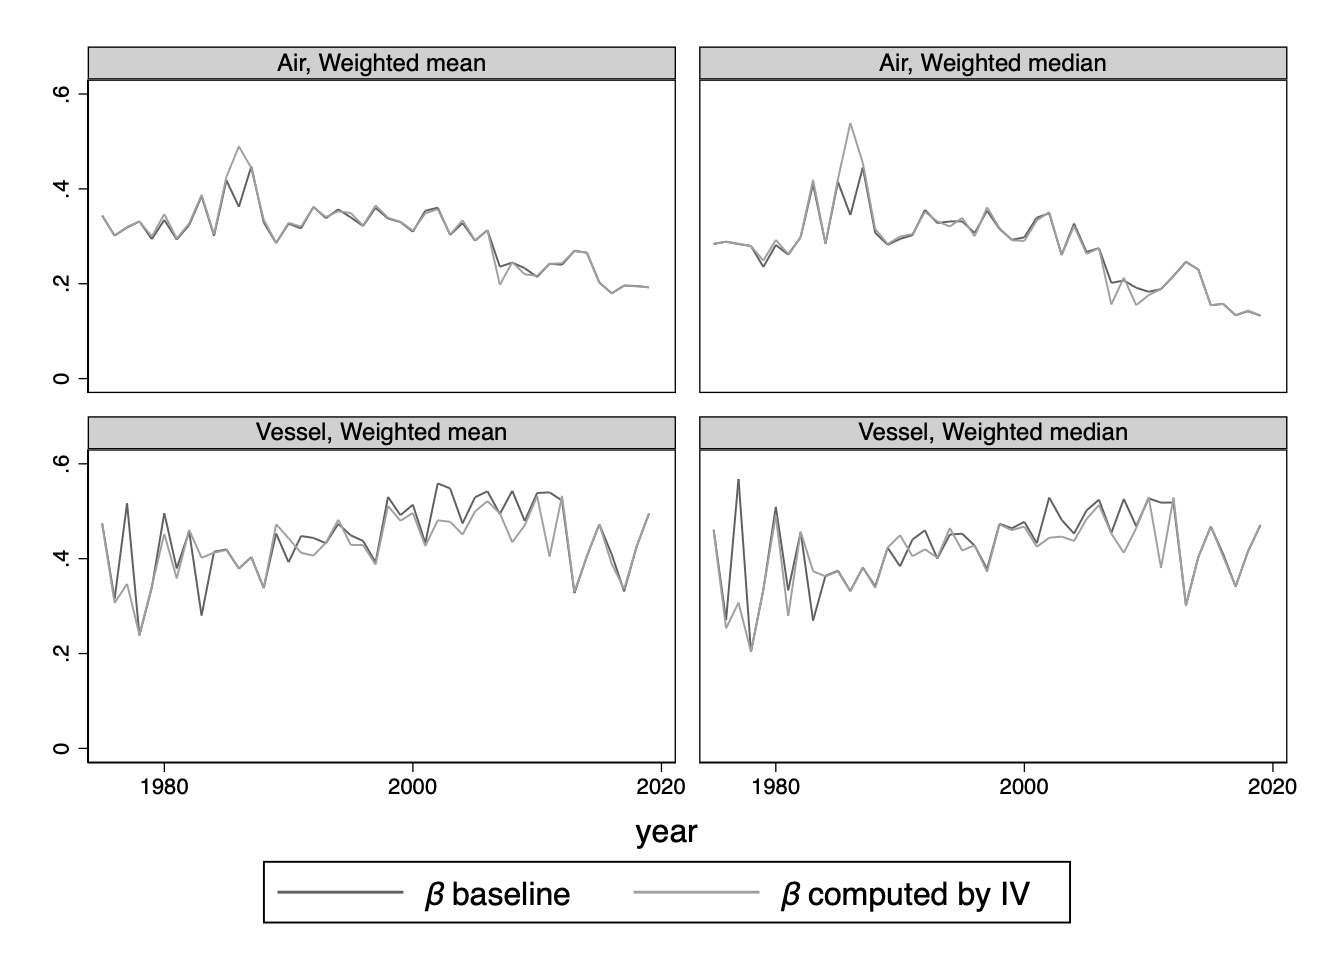
\includegraphics[height=8cm]
{scatter_chronology_baseline_IV_ref1_y_5_3.png}
\end{center}
\end{figure}

%However, we consider as a reasonable assumption that the exporting firm cannot influence the international transport cost sector, that would imply a causal effect of the firm's prices on the transport costs value, except in the choice between air and vessel transport (that is beyond our scope of analysis).
%Otherwise stated, conditional to an export price and a transport mode, the gap between the export price declared to the custom data and the import price recorded by the US administration is beyond the firm's control.
%In this respect, we are confident that our estimation strategy is immune from endogeneity problems.


\subsubsection{Robustness to aggregation}

Current data are available at the 10-digit level for products (HS10).
Theoretically, they should be available from 1989. 
But because of the COVID situation, it was only possible to get 1997-1999 and 2001-2019.
Yet, as \ref{tab: baseline10} shows, the results are similar when using 10-digit product and 5-digit products. 

\begin{table}[htbp]
	\centering
	\caption{Transport costs estimates: robustess to agregation} \vspace{5mm} \label{tab:baseline10}
	\begin{tabular}{lllll}
\cline{1-5}
\multicolumn{1}{c}{} &
  \multicolumn{2}{|c}{air} &
  \multicolumn{2}{c}{ves} \\
\multicolumn{1}{c}{} &
  \multicolumn{1}{|r}{10/3-digit} &
  \multicolumn{1}{r}{5/3-digit} &
  \multicolumn{1}{r}{10/3-digit} &
  \multicolumn{1}{r}{5/3-digit} \\
\cline{1-5}
\multicolumn{1}{l}{\textbf{Data}} &
  \multicolumn{1}{|r}{} &
  \multicolumn{1}{r}{} &
  \multicolumn{1}{r}{} &
  \multicolumn{1}{r}{} \\
\multicolumn{1}{l}{\hspace{1em}Mean} &
  \multicolumn{1}{|r}{} &
  \multicolumn{1}{r}{} &
  \multicolumn{1}{r}{} &
  \multicolumn{1}{r}{} \\
\multicolumn{1}{l}{\hspace{2em}{$\#$ obs.}} &
  \multicolumn{1}{|r}{184,791} &
  \multicolumn{1}{r}{41,541} &
  \multicolumn{1}{r}{159,976} &
  \multicolumn{1}{r}{39,661} \\
\multicolumn{1}{l}{\hspace{2em}{$\#$ sectors}} &
  \multicolumn{1}{|r}{217} &
  \multicolumn{1}{r}{217} &
  \multicolumn{1}{r}{226} &
  \multicolumn{1}{r}{226} \\
\multicolumn{1}{l}{\hspace{2em}{$\#$ origin countries}} &
  \multicolumn{1}{|r}{210} &
  \multicolumn{1}{r}{210} &
  \multicolumn{1}{r}{205} &
  \multicolumn{1}{r}{205} \\
\multicolumn{1}{l}{\hspace{1em}{\textit{Obs. transport costs $(p/\widehat{p}-1)$ (in $\%$)}}} &
  \multicolumn{1}{|r}{} &
  \multicolumn{1}{r}{} &
  \multicolumn{1}{r}{} &
  \multicolumn{1}{r}{} \\
\multicolumn{1}{l}{\hspace{2em}Mean} &
  \multicolumn{1}{|r}{2.5} &
  \multicolumn{1}{r}{2.7} &
  \multicolumn{1}{r}{4.2} &
  \multicolumn{1}{r}{4.2} \\
\multicolumn{1}{l}{\hspace{2em}Median} &
  \multicolumn{1}{|r}{1.2} &
  \multicolumn{1}{r}{1.6} &
  \multicolumn{1}{r}{3.1} &
  \multicolumn{1}{r}{3.1} \\
\multicolumn{1}{l}{\hspace{2em}Std. dev.} &
  \multicolumn{1}{|r}{5.3} &
  \multicolumn{1}{r}{4.5} &
  \multicolumn{1}{r}{4.3} &
  \multicolumn{1}{r}{3.7} \\
\multicolumn{1}{l}{\hspace{1em}{\textit{Export price in USD per kg (\textit{$\widehat{p}$})}}} &
  \multicolumn{1}{|r}{} &
  \multicolumn{1}{r}{} &
  \multicolumn{1}{r}{} &
  \multicolumn{1}{r}{} \\
\multicolumn{1}{l}{\hspace{2em}Mean} &
  \multicolumn{1}{|r}{39,354} &
  \multicolumn{1}{r}{16,734} &
  \multicolumn{1}{r}{41} &
  \multicolumn{1}{r}{16} \\
\multicolumn{1}{l}{\hspace{2em}Median} &
  \multicolumn{1}{|r}{352} &
  \multicolumn{1}{r}{246} &
  \multicolumn{1}{r}{6} &
  \multicolumn{1}{r}{5} \\
\multicolumn{1}{l}{\hspace{2em}Std. dev.} &
  \multicolumn{1}{|r}{369,112} &
  \multicolumn{1}{r}{101,111} &
  \multicolumn{1}{r}{1,781} &
  \multicolumn{1}{r}{176} \\
\multicolumn{1}{l}{{\textbf{Model (B)}}} &
  \multicolumn{1}{|r}{} &
  \multicolumn{1}{r}{} &
  \multicolumn{1}{r}{} &
  \multicolumn{1}{r}{} \\
\multicolumn{1}{l}{\hspace{1em}{\textit{Multiplicative term (in $\%$)} ($\widehat{\tau}^{adv}$)}} &
  \multicolumn{1}{|r}{} &
  \multicolumn{1}{r}{} &
  \multicolumn{1}{r}{} &
  \multicolumn{1}{r}{} \\
\multicolumn{1}{l}{\hspace{2em}Mean} &
  \multicolumn{1}{|r}{1.7} &
  \multicolumn{1}{r}{2.0} &
  \multicolumn{1}{r}{1.7} &
  \multicolumn{1}{r}{2.1} \\
\multicolumn{1}{l}{\hspace{2em}Median} &
  \multicolumn{1}{|r}{1.4} &
  \multicolumn{1}{r}{1.7} &
  \multicolumn{1}{r}{1.5} &
  \multicolumn{1}{r}{1.8} \\
\multicolumn{1}{l}{\hspace{2em}Std. dev.} &
  \multicolumn{1}{|r}{1.4} &
  \multicolumn{1}{r}{1.9} &
  \multicolumn{1}{r}{1.2} &
  \multicolumn{1}{r}{1.6} \\
\multicolumn{1}{l}{\hspace{1em}{\textit{Additive term (in $\%$)} ($\widehat{t}/\widetilde{p}$)}} &
  \multicolumn{1}{|r}{} &
  \multicolumn{1}{r}{} &
  \multicolumn{1}{r}{} &
  \multicolumn{1}{r}{} \\
\multicolumn{1}{l}{\hspace{2em}Mean} &
  \multicolumn{1}{|r}{1.2} &
  \multicolumn{1}{r}{1.0} &
  \multicolumn{1}{r}{2.3} &
  \multicolumn{1}{r}{2.1} \\
\multicolumn{1}{l}{\hspace{2em}Median} &
  \multicolumn{1}{|r}{0.3} &
  \multicolumn{1}{r}{0.4} &
  \multicolumn{1}{r}{1.5} &
  \multicolumn{1}{r}{1.6} \\
\multicolumn{1}{l}{\hspace{2em}Std. dev.} &
  \multicolumn{1}{|r}{3.0} &
  \multicolumn{1}{r}{2.2} &
  \multicolumn{1}{r}{3.6} &
  \multicolumn{1}{r}{2.5} \\
\multicolumn{1}{l}{\hspace{1em}{\textit{Additive term in USD per kg ($\widehat{t}$)}}} &
  \multicolumn{1}{|r}{} &
  \multicolumn{1}{r}{} &
  \multicolumn{1}{r}{} &
  \multicolumn{1}{r}{} \\
\multicolumn{1}{l}{\hspace{2em}Mean} &
  \multicolumn{1}{|r}{1.54} &
  \multicolumn{1}{r}{1.43} &
  \multicolumn{1}{r}{0.12} &
  \multicolumn{1}{r}{0.11} \\
\multicolumn{1}{l}{\hspace{2em}Median} &
  \multicolumn{1}{|r}{1.38} &
  \multicolumn{1}{r}{1.26} &
  \multicolumn{1}{r}{0.12} &
  \multicolumn{1}{r}{0.10} \\
\multicolumn{1}{l}{\hspace{2em}Std. dev.} &
  \multicolumn{1}{|r}{1.07} &
  \multicolumn{1}{r}{1.06} &
  \multicolumn{1}{r}{0.10} &
  \multicolumn{1}{r}{0.10} \\
\multicolumn{1}{l}{\hspace{1em}$\widehat{\beta}$:  \textit{Share of additive costs}} &
  \multicolumn{1}{|r}{} &
  \multicolumn{1}{r}{} &
  \multicolumn{1}{r}{} &
  \multicolumn{1}{r}{} \\
\multicolumn{1}{l}{\hspace{2em}Mean} &
  \multicolumn{1}{|r}{0.25} &
  \multicolumn{1}{r}{0.23} &
  \multicolumn{1}{r}{0.50} &
  \multicolumn{1}{r}{0.47} \\
\multicolumn{1}{l}{\hspace{2em}Median} &
  \multicolumn{1}{|r}{0.16} &
  \multicolumn{1}{r}{0.19} &
  \multicolumn{1}{r}{0.53} &
  \multicolumn{1}{r}{0.45} \\
\multicolumn{1}{l}{\hspace{2em}Std. dev.} &
  \multicolumn{1}{|r}{0.24} &
  \multicolumn{1}{r}{0.19} &
  \multicolumn{1}{r}{0.26} &
  \multicolumn{1}{r}{0.27} \\
\cline{1-5}
\end{tabular}

	\begin{tablenotes}
		\tiny
		\item Statistics for 1997-1999 and 2002-2019
		\item Statistics are obtained weighting each observation by its value relative to total trade flows.
		\item \textbf{Model (a): With ad-valorem transport costs only}
		\item \textbf{Model (b): With additive and ad-valorem transport costs}
	\end{tablenotes}
\end{table}
   

\begin{figure}[htbp]
	\caption{Transport cost time trends: robustness to agregation}
	\label{fig:comp_IV_SITC5}
	\begin{center}
		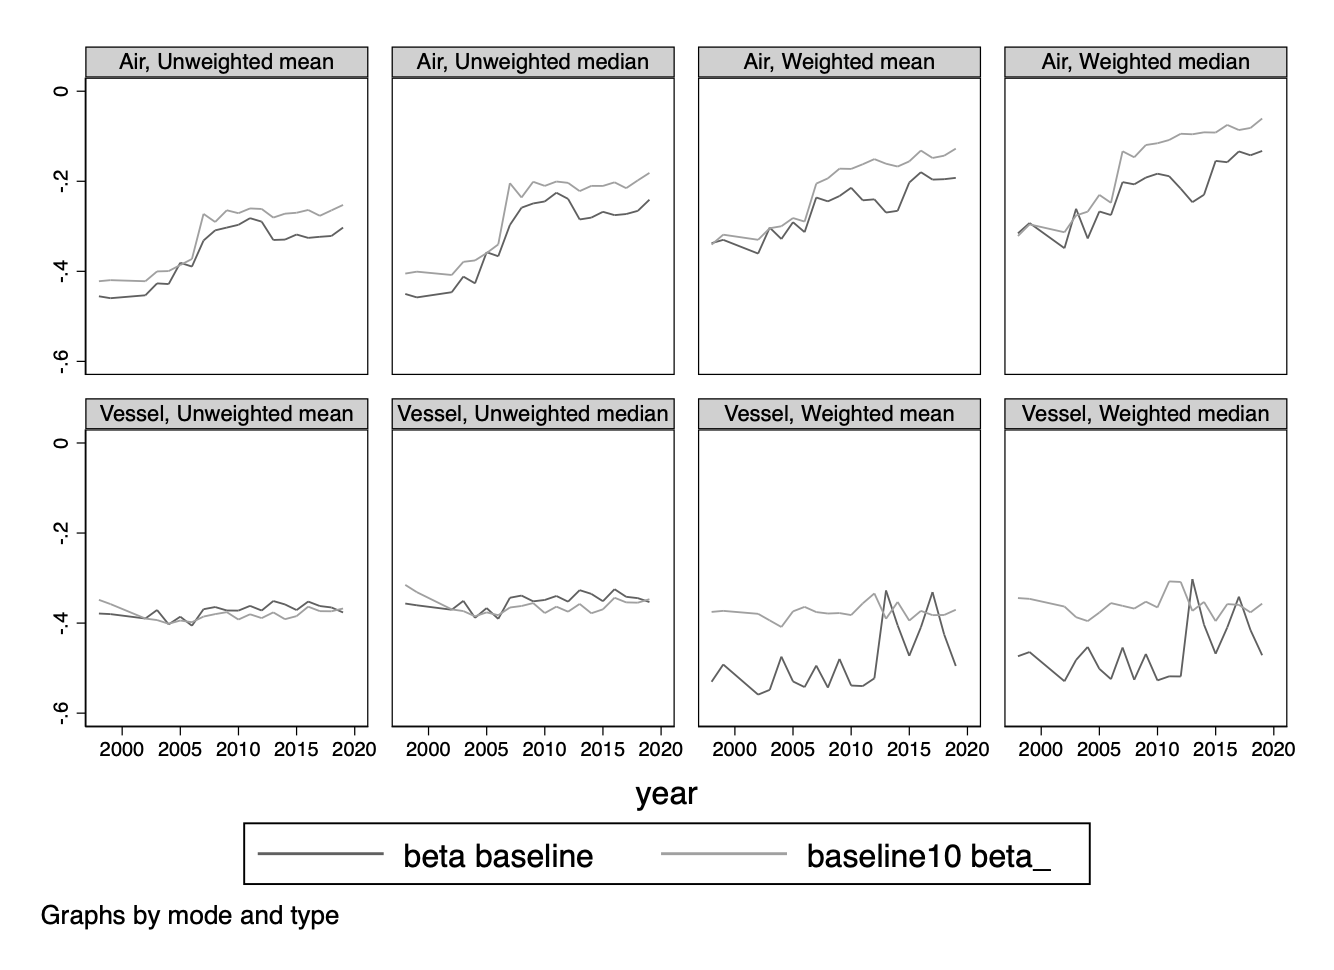
\includegraphics[height=8cm]{scatter_chronology_baseline_baseline10.png}
	\end{center}
\end{figure}


\section{Additive costs and transport costs time trends}\label{sec:results_trends}

In this section, we investigate the underlying sources behind the downward trend of international transport costs, by identifying the respective roles of the reduction in ``pure'' transport costs and changes in trade composition effects. As underlined by \cite{hummels2007}, the time trend of international transport costs depends on both the evolution of per product and per partner (``pure'') transport costs and the evolution of the composition of trade.
Total transport costs may thus have decreased over time because the share of neighboring countries in total US trade or the share of goods cheaper to transport has increased, independently of any change in transport costs \textit{per se}.
As emphasized by \cite{Hummels_1999} and \cite{hummels2007}, it is hence necessary to eliminate the composition effects of trade flows to isolate the evolution of pure international transport costs.
Specifically, Hummels's (2007) results\nocite{hummels2007} underlie the view that trade composition effects partially compensate the reduction in pure transport costs, thereby attenuating the downward trend in overall (observed) transport costs since 1974.
Our own results tend to challenge this view, as we further show.

\paragraph{A word on Hummels' methodology} At this point, let us make a brief summary of Hummels' methodology\nocite{hummels2007}.
He starts from the following specification of the ratio of destination to origin prices modelled as $p_{ikt} = \widetilde{p}_{ikt}+\frac{f_{ikt}}{ \widetilde{p}_{ikt}},$ with $f_{ikt}$ the shipping charge per kg shipped (for a given product $k$ imported from country $i$ in year $t$).
Further, and as in \cite{hummels_skiba}, \cite{hummels2007} writes the per kg shipping charge as $f_{ikt}=\widetilde{p}_{ikt}^{1-\beta}X_{ikt}$, where $X_{ikt}$ represents other costs shifters (distance, port quality, etc.) Accordingly, his transport cost measure $TC_{ikt}$ writes is written as:

\begin{equation}
TC_{ikt}\equiv \frac{p_{ikt}-\widetilde{p}_{ikt}}{\widetilde{p}_{ikt}} = \widetilde{p}_{ikt}^{-\beta}X_{ikt} \label{eq:Hummel_benchmarkeq}
\end{equation}

As already noticed, $\beta$ can be interpreted as the elasticity of transport costs to the export price (in absolute value), also equal to the share of additive costs in total transport costs.
Equation (\ref{eq:Hummel_benchmarkeq}) is the baseline specification from which \cite{hummels2007} decomposes the changes in transport costs over time between trade composition effects and changes in ``pure'' transport costs, as described in more detail in Appendix \ref{app:compare_Hummels}.
In doing so, \cite{hummels2007} implicitly assumes $\beta$ constant across the triplet origin country origin/product/year.
Put differently, this means that the share of additive costs in total costs does not vary across these dimensions.

\paragraph{Challenging the $\beta$'s constancy assumption} As Figure \ref{fig:part_cout_additif} (based on the yearly estimates of transport costs averaged over the country/sector dimension) suggests, the share of additive costs is rather varying over time, in both transport modes.
%In light of this, one may wonder about the constancy of the share of additive costs along the pair product/origin country hypothesized by \cite{hummels2007}.
We investigate this point deeper by reporting the histogram of the distribution of the share of additive costs in total costs.
To do so, we start from Equation (\ref{eq:base_estimee}) with the trade costs measure on the left-hand side, from which we deduce the formulae to get the elasticity of transport costs to the export price on a per product-year-country basis, i.e.
$\beta$, according to:
\begin{eqnarray*}
\beta_{ikt} &\equiv& -\frac{\partial TC_{ikt}}{\partial \widetilde{p}_{ikt}}\frac{\widetilde{p}_{ikt}}{TC_{ikt}} \\
&=& \frac{\widehat{t}_{is(k)t}/\widetilde{p}_{ikt}}{\widehat{t}_{is(k)t}/\widetilde{p}_{ikt}+\widehat{\tau}_{is(k)t}-1},
\end{eqnarray*}

\textbf{ajoute un s(k) sur nos valeurs estimees}

\noindent making use of our first-stage estimates for both the additive and the ad-valorem components ($\widehat{t}_{is(k)t}$ and $\widehat{\tau}_{is(k)t}$). The histogram of the distribution of the estimated $\beta_{ikt}$ is reported in Figure \ref{fig:histogram_beta}, in panels (a) and (b) for air and maritime transport respectively.


\begin{figure}[htbp]
\caption{Share of additive costs in total costs: Histogram}
\label{fig:histogram_beta}
\begin{center}
\begin{tabular}{cc}
%{\small (a) Air } & {\small (b) Vessel}\\
\includegraphics[width=3.0in, height=2.5in]{"Etude_beta_pondere_(a) Air transport".jpg}
& \includegraphics[width=3.0in,height=2.5in]{"Etude_beta_pondere_(b) Vessel transport".jpg} \\
\multicolumn{2}{l}{{\footnotesize Notes: Distribution of $\beta_{ikt}$ over the triplet (year,product,country), weighted by share of yearly value of flow.}}\\
\end{tabular}
\end{center}
\end{figure}

As displayed in Figure \ref{fig:histogram_beta}, for both transport modes the distribution of $\beta_{ikt}$ over the triplet (year, product, origin country) is smoothly distributed over the interval $[0,1]$, with a mode of the distribution standing around 0.3-0.4 depending on the transport mode, consistently with our previous findings.
This stands in sharp contrast with the assumption made by  \cite{hummels_skiba} or \cite{hummels2007}, which would imply a distribution concentrated on a single point.
Rather, this suggests that the elasticity of transport costs to the export price, or equivalently the share of additive costs in total costs, is varying across time, product and country partner.\footnote{We have checked that it is also the case when we look at the distribution over the range of origin countries or products, for a given year.
These results are not reported for sake of space, but are available upon request to the authors.} In the next section, we shed light on the role of this result in the analysis of the underlying sources of the overall transport costs trend patterns, between trade composition effects and pure transport costs.

\subsection{Empirical specification}

Based on the above results, we provide a decomposition of the transport costs trends between the trade composition effects and the ``pure'' transport costs time trends, which explicitly takes into account the varying share of additive costs over time, country partner and product.\footnote{See Appendix \ref{app:compare_Hummels} for a detailed comparison of Hummel's (2007) methodology and ours.} An important contribution of the paper is to show the crucial role of this (empirically relevant) assumption, as it notably modifies the conclusions relative to the role of trade composition effects.
We start with the presentation of our estimation strategy before turning to the results.\smallskip

\subsubsection{Estimation strategy}

The estimation carried out in Section \ref{sec:results_decomposition} provides us with the additive and ad-valorem measures of international transport costs (Equation (\ref{eq:model_IetA})), which vary over time, product and origin country (i.e., $\widehat{t}_{ikt}$ and $\widehat{\tau}_{ikt}$).
Starting from these values, for each additive and multiplicative cost component (by transport mode) we extract the pure transport cost measure by the mean of a time fixed effect.
Precisely, we extract the changes over time in the pure transport cost dimension by assuming a composition of trade flows by country partner and product that is constant throughout the period, and equal to the one observed in 1974.
We conduct the same analysis on an overall transport costs measure, built by combining the two estimated components (additive and iceberg) in a unified measure of transport costs.\footnote{Note that the unfitted total transport costs are virtually the same as those reported in Figure \ref{fig:Trends_in_TC}, but reported from another perspective (basis 100 in year 1974).} The objective is to obtain six time series, all built as indices with the reference value 100 in 1974: three time series for the unfitted transport costs measures $\{\Gamma^{add, raw}_t, \Gamma^{adv, raw}_t, \Gamma^{tc, raw}_t \}$  (additive, ad-valorem and total cost respectively), and three series for the fitted values $\{\Gamma^{add}_t, \Gamma^{adv}_t, \Gamma^{tc}_t \}$ (additive, ad-valorem and total cost respectively).

One advantage of this method is that it yields measures of transport costs (fitted and unfitted) that are easily comparable between transport modes and transport cost components.
For each cost component (additive and ad-valorem) as well as for the total transport cost, comparing the unfitted measure and the fitted measure (composition effects excluded) makes it possible to identify if the decrease observed over the period in the unfitted series is due to trade composition effects (for instance, changes in the country partners, in the type/quality of products traded), or if it is the pure transport costs (for instance, insurance or handling costs) that have reduced over time. For sake of reading clarity, we describe the method to extract these series in Appendix \ref{app:comp-effects}, and we now turn to the results.



\subsection{Characterizing the time trends in transport costs}
Figure \ref{fig:totalTC_compeffects_excl} reports the results for all types of goods.\footnote{In the Online Appendix, we report the results at a more disaggregated level, distinguishing between primary and manufacturing goods.} In panels (a), (b) and (c) we report the time changes of the ad-valorem costs, the additive costs and the total costs respectively, for air transport (starting from the reference value 100 in 1974).
Panels (d), (e) and (f) report the results for vessel.
In each panel, we report the evolution of transport costs for both the unfitted (plain blue line) and the fitted (dotted red line) measures.


\begin{figure}[htbp]
\caption{Transport costs (with and without composition effects)}
\label{fig:totalTC_compeffects_excl}
\begin{center}
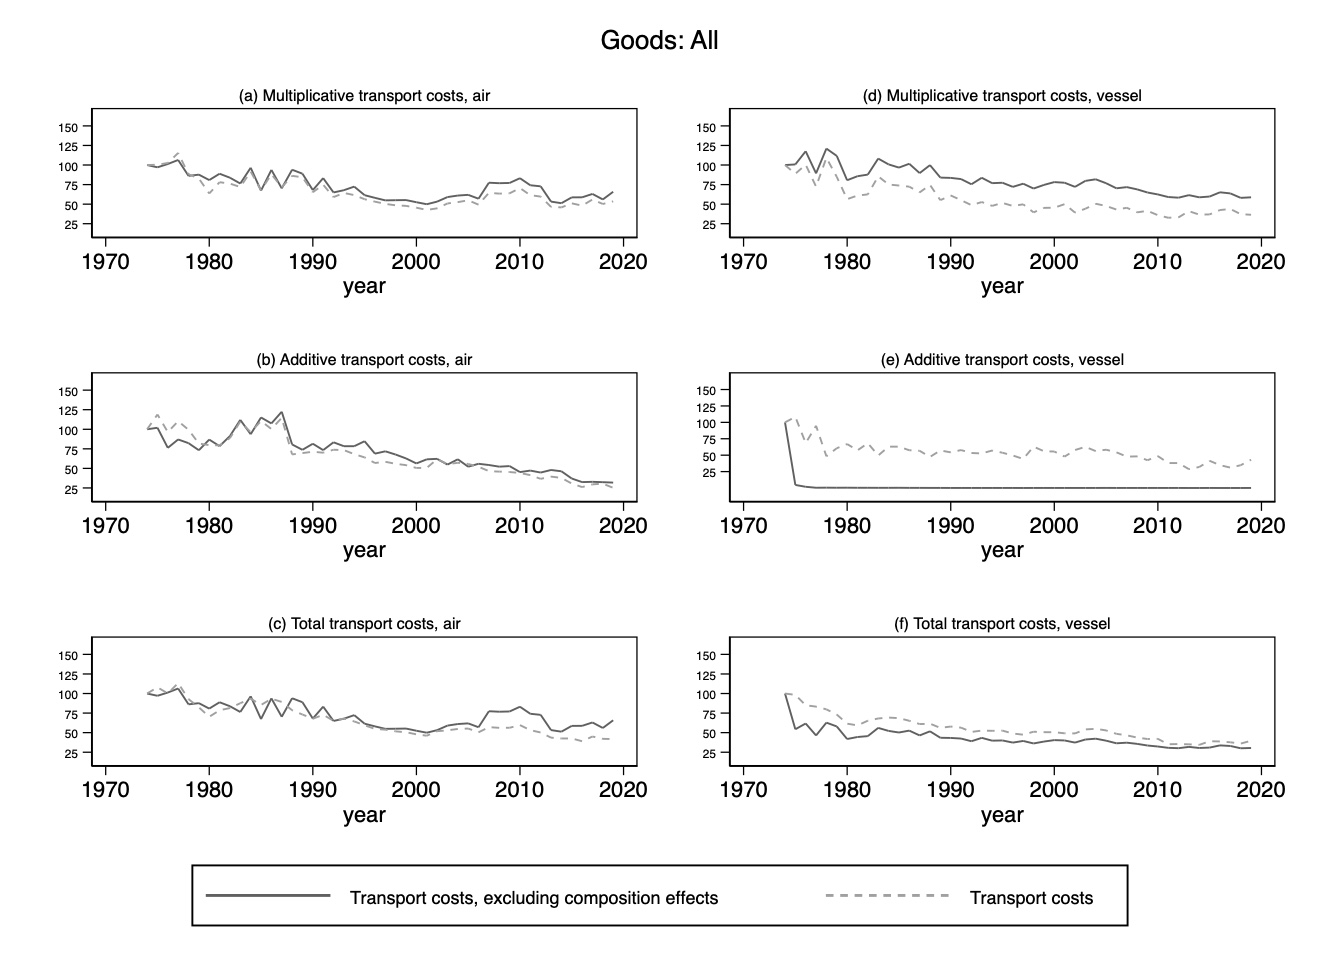
\includegraphics[height=4in]
{graph_composition_all.jpg}
\end{center}
\end{figure}

Three main results emerge from Figure \ref{fig:totalTC_compeffects_excl}.
First, in accordance with Figure \ref{fig:Trends_in_TC}, we find that international transport costs have substantially decreased over the period, for both transport modes (Panels (c) and (f)).
International transport costs were reduced by 50\% between 1974 and 2019 in air shipping, and by 60\% in maritime shipping.
This stands in line with the related literature (see \citealp{Hummels_1999}; \citealp{Lafourcade_Thisse}).
Second, the magnitude of the decrease is roughly of the same order for both for the ad-valorem and the additive components (Panels (a), (b), (d) and (e)).
Further, the transport cost reduction is much smoother in maritime transport, while air transport shows more volatility in the trend pattern, in particular in the 1980s and the 2000s.
Third, and most importantly, we find that composition effects do not play a major role in accounting for the time trend of overall transport costs.
Inspecting the panels of Figure \ref{fig:totalTC_compeffects_excl} for air transport (panels (a) to (c)), we do not find much evidence of a substantial trend difference between the unfitted transport costs measure and the pure transport costs.
For all three series (additive, ad-valorem and overall transport costs), the dotted and the plain line follow closely, almost every year throughout the period.
Air transport costs were reduced by 50\% between 1974 and 2019, which is mainly attributable to a reduction in the transport costs ``per se''.
Composition effects are stronger in vessel transport, for all three series (Figure \ref{fig:totalTC_compeffects_excl}, panels (d) to (f)): they amplify the reduction in ``pure'' transport costs at the beginning of the period, in the 1970s (the dotted line is below the plain line, and the gap is increasing). Afterwards, the dotted line remains below the plain line, but the gap between the two remains roughly constant across years, indicating that the amplification effect does not strengthen anymore: the two trends are similar.
Considering the raw series (plain line), maritime transport costs have decreased by 60\% over the period, which can be decomposed into a 50\% decrease in transport costs ``per se'' (dotted line), and a 10\% reduction that comes from composition effects (the difference of the two).
This is particularly the case for the multiplicative component (panel (d)).\smallskip




\subsection{Time trends in transport costs and the modeling of the additive component}

The last results stand in sharp contrast with \cite{hummels2007}, who finds that trade composition effects do matter, as they partially offset the reduction in the pure transport costs for both air and maritime shipping.
If anything, we find the opposite result here: Trade composition effects do not matter much in accounting for the downward trend of observed international transport costs, and when they do, they tend to amplify (rather than reduce) the downward pattern.
This drives us to investigate this difference further.
As we explain in more detail in Appendix \ref{app:comp-effects}, our empirical strategy differs from \cite{hummels2007} in one main dimension.
Our characterization of the time trends in transport costs starts from our estimates of both the additive and the ad-valorem components (obtained in Section \ref{sec:results_decomposition}), as well as for the overall transport cost (rather than the actual cif-fas price gap).
Consequently, our methodology lets the ratio between the additive and the ad-valorem components of transport costs vary over the three time-product-partner country dimensions.
%By contrast, \cite{hummels2007} does not take into account the changes in the additive transport cost component, attributing this to a change in the composition of the bundle over time (per country-commodity).
This turns out to be of primary importance in the disentangling, in the time trend of transport costs, of what comes from the trade composition effects and what comes from changes in the pure transport cost dimension, as we show below.

To establish this point clearly, we replicate the method adopted by \cite{hummels2007} exposed above on our database (which is the same as his until 2004).
The results are reported in Figure \ref{fig:comp_effects_as_in_Hummels}.
The dotted line labeled ``expenditure/import value'' represents the unfitted measure of transport costs ($TC_t$ in the above terminology) and the plain line labeled ``fitted ad-valorem rate'' is the measure of ``pure'' transport costs, i.e.
composition effects excluded ($\widehat{TC}_t$).
In Panels (a) (for air) and (b) (for vessel), we report the transport costs measures (fitted and unfitted) expressed as a percentage of the export price, as in \cite{hummels2007}.\footnote{Unsurprisingly, this accords with \cite{hummels2007} results, see his Figures 5 (for air) and 6 (for vessel).} To ease the interpretation of the trends, we express them as indices with the reference value 100 in 1974, in Panels (c) and (d) for air and vessel respectively.

\begin{figure}[htbp]
\caption{Characterizing the time trends: applying Hummel's (2007) method }
\label{fig:comp_effects_as_in_Hummels}
\begin{center}
\begin{tabular}{cc}
{\small (a) Ad-valorem air freight} & {\small (b) Ad-valorem vessel freight}\\
\multicolumn{2}{c}{{\small In percent of the export price}} \\
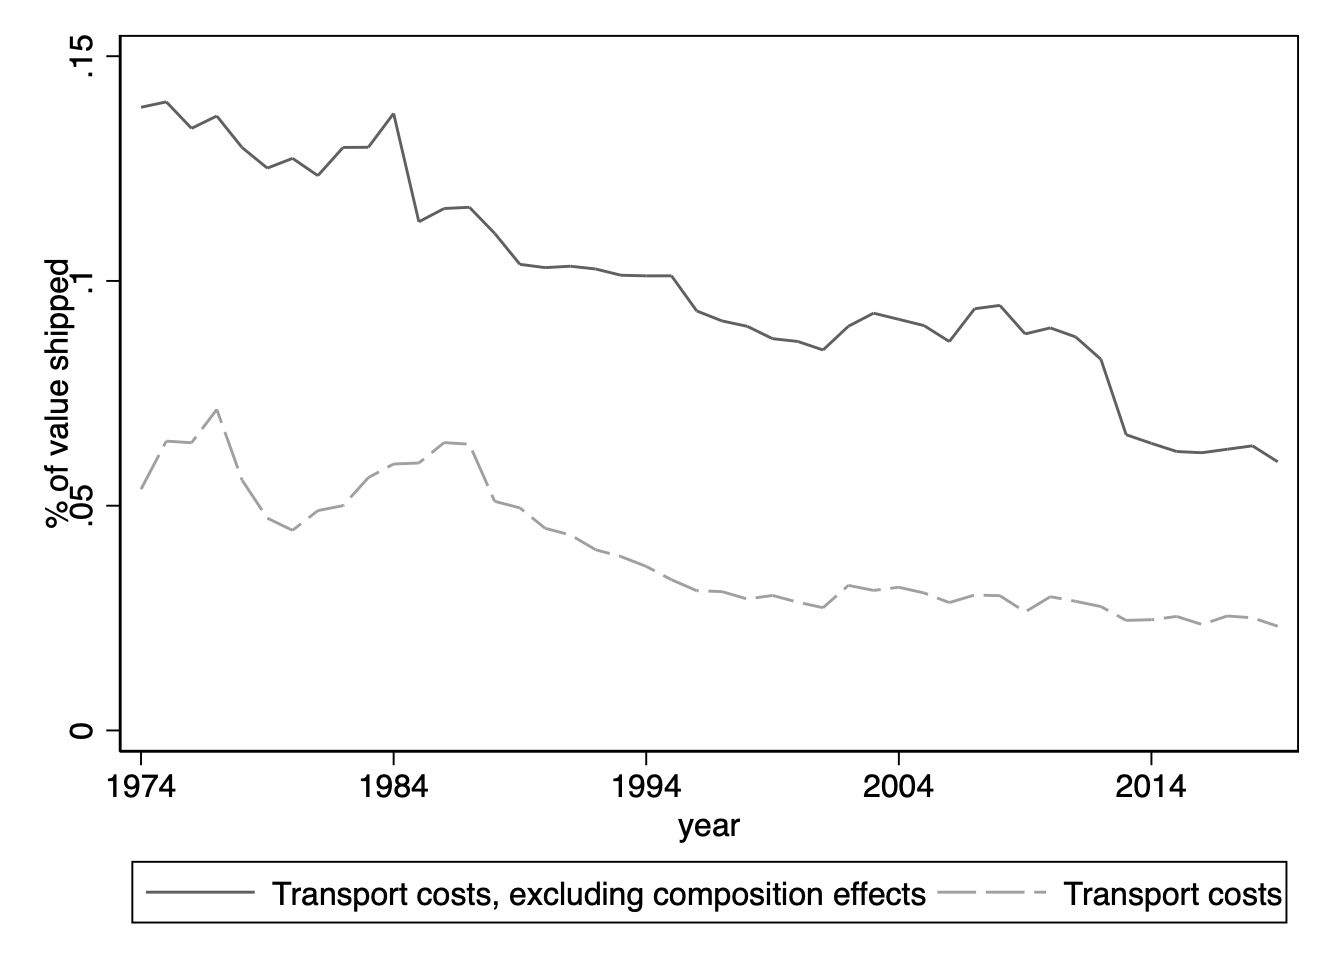
\includegraphics[width=2.5in, height=1.8in]{figure5_comme_hummels.jpg}
& 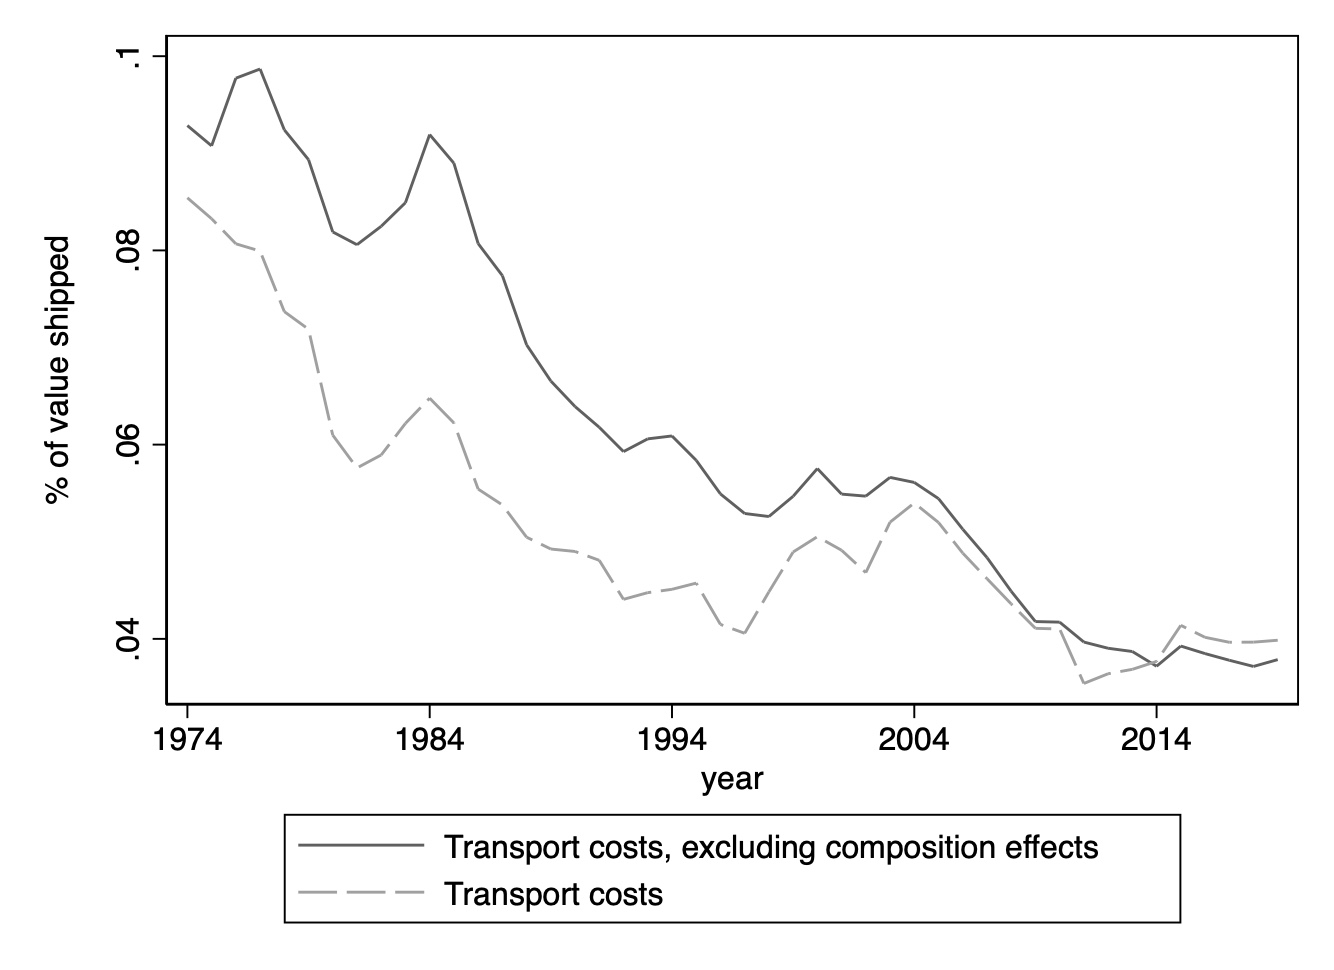
\includegraphics[width=2.5in,height=1.8in]{figure6_comme_hummels.jpg} \\
{\small (c) Ad-valorem air freight} & {\small (d) Ad-valorem vessel freight}\\
\multicolumn{2}{c}{{\small As indices with reference value 100 in 1974} }\\
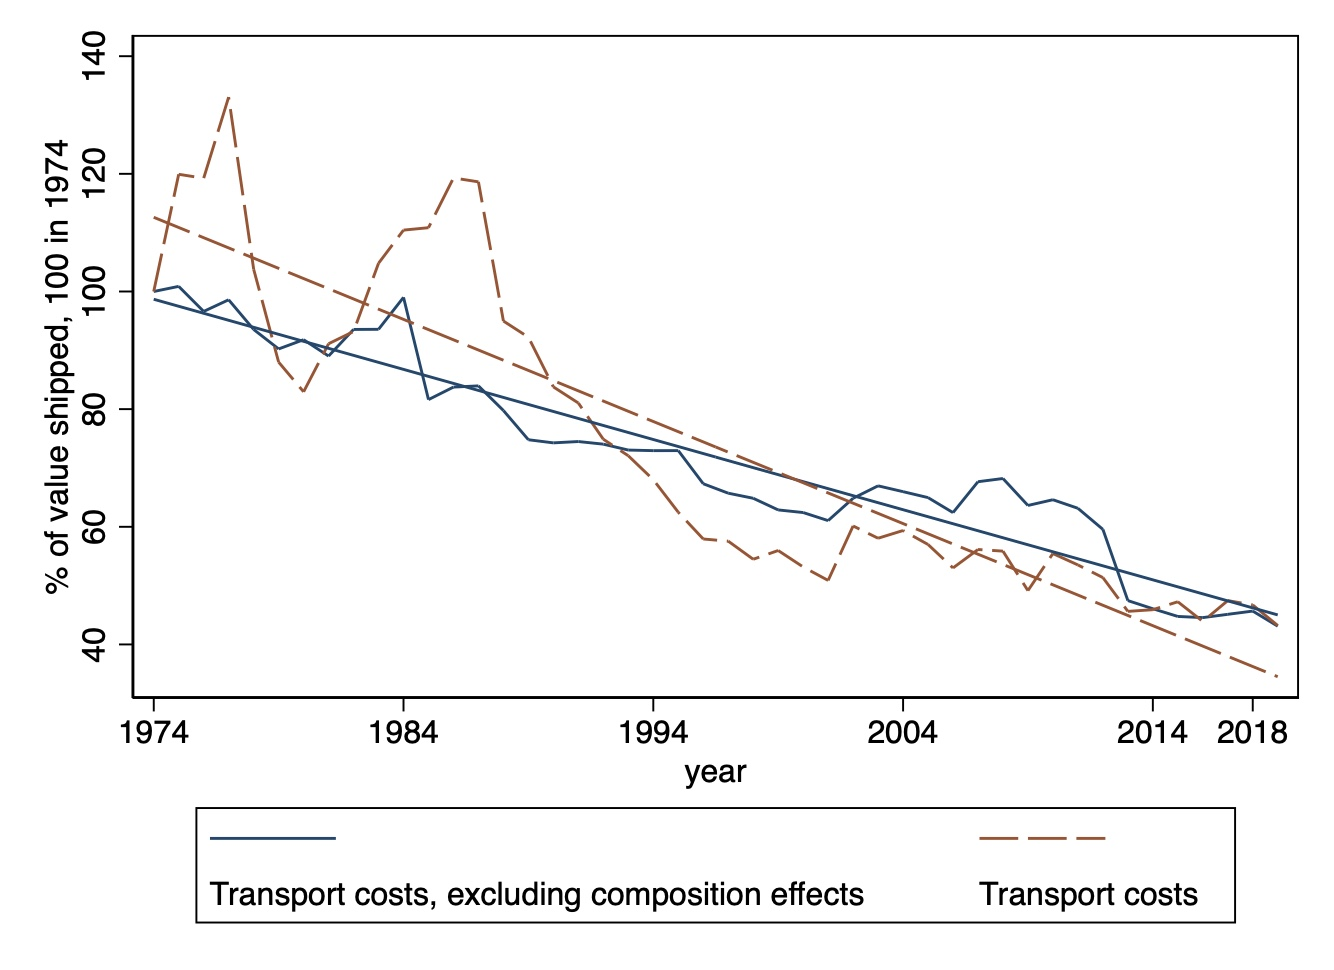
\includegraphics[width=2.5in, height=2in]{figure5_comme_hummels_base100.jpg}
& 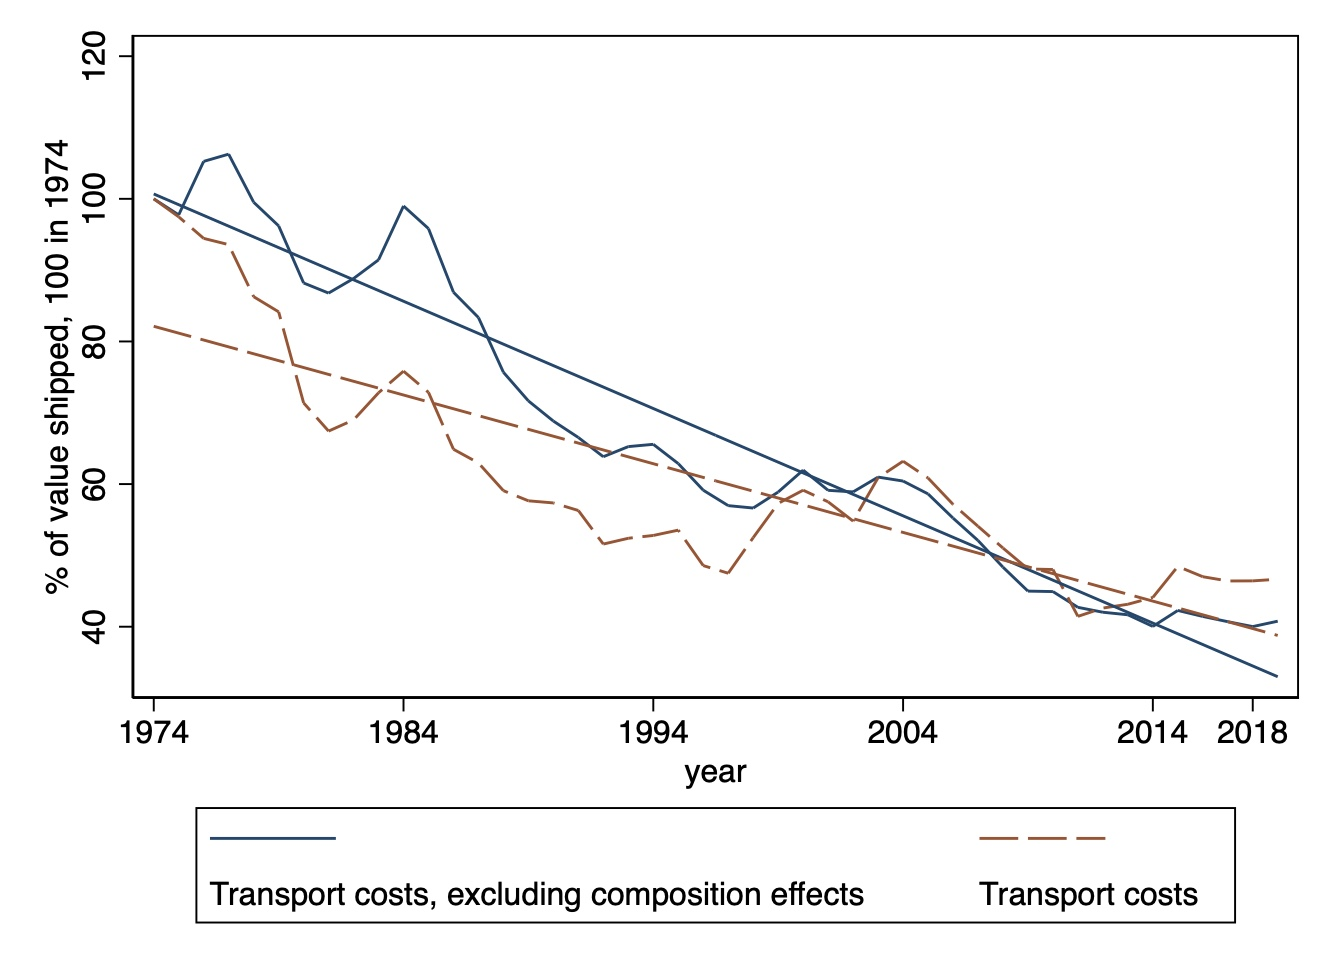
\includegraphics[width=2.5in,height=2in]{figure6_comme_hummels_base100.jpg} \\
\end{tabular}
\end{center}
\end{figure}

These results stand in sharp contrast with the ones obtained with our methodology and reported in Figure \ref{fig:totalTC_compeffects_excl}.
Applying \cite{hummels2007} method, we find that the composition effects tend to partly offset the decrease in transport costs in both air and vessel shipping, as the downward trend is of higher magnitude for the fitted rate (plain line) than the unfitted rate (dotted line), especially for vessel (Panel (d)).
Yet, this result is overturned when we allow for more flexibility in the role of the additive component, as indicated in Figure \ref{fig:totalTC_compeffects_excl}, Panels (c) and (f).\medskip


Assuming a varying share of the additive component over time, product and country partner indeed modifies the decomposition of the trend reduction of transport costs between the one attributable to trade composition effects and the reduction in the ``pure'' transport costs.
In both air and vessel transports, we thus find that this last dimension is the main driver of the reduction in international transport costs observed over time, in particular in air transport.
Complementing the findings of Section \ref{sec:results_decomposition}, these results highlight the importance of integrating the additive dimension of international transport costs, with the aim here of characterizing their time trends.




\section{The role of additive cost: Theoretical insights}\label{sec:theory}

\textbf{ATTENTION AJUSTER LES FIGURES ET CHIFFRES A NOUVELLE CALIBRATION}

In this section, we explore the implications of our empirical results on theoretical grounds. While the whole bulk of the trade literature investigates the role of trade costs modelled as ad-valorem costs (e.g., iceberg trade costs), not much is said about the role of the additive component. One potential explanation is the lack of empirical estimates about the size of additive costs. Our results may thus usefully palliate this limitation. Specifically, we make use of our empirical results to investigate the welfare consequences of a reduction in international transport costs, when such a reduction also occurs through a reduction in the additive component. \cite{Irrazabal_2015}, \cite{sorensen2014} and \cite{Lashkaripour_JIE2020} have preceded us on this issue. We differentiate from them in the following way. \cite{sorensen2014} explores the welfare effects of a trade costs reduction depending on whether they are either fully ad-valorem or fully additive. In contrast, we provide a quantification of such welfare gains, as in \cite{Irrazabal_2015} or \cite{Lashkaripour_JIE2020}. To do so, we rely on our empirical estimates of the transport costs values, that induce a combined decrease in both the ad-valorem and the additive components over the last decades. In a partial-equilibrium model with perfect competition, \cite{Lashkaripour_JIE2020} obtains that welfare gains are not substantially different whether the transport cost decrease implies an additive component or not. This stands in contrast with the conclusion reached by \cite{sorensen2014} (analytically) and \cite{Irrazabal_2015} (quantitatively) in M\'{e}litz' type models. Anticipating on our results, we also share the result, that the transport cost reduction implies substantially larger welfare gains when they are achieved through a reduction in the additive component. As first explanation, it should be noted that, in \cite{Lashkaripour_JIE2020}'s paper, the case with additive costs relies on a share of additive costs that remains negligible. In this context, one might expect that whether additive costs are present or not makes little difference. As underlined by \cite{Lashkaripour_JIE2020}, a second explanation may rely on the modeling framework. While \cite{Lashkaripour_JIE2020} models a perfectly competitive multi-sector model, we as in \cite{sorensen2014} and \cite{Irrazabal_2015} adopt a model with monopolistic competition and firm selection \`{a} la \cite{melitz} or \cite{chaney2008}. In this setting, we indeed show that additive costs do modify the selection of firm on both the domestic and the export markets, e.g the extensive margin of trade, whose role in the welfare gains of trade liberalization lies at the heart of the New Trade models  \`{a} la \cite{melitz}. Put differently, leaving aside the selection issue leads to underestimate the welfare gains that can be achieved by a reduction in the additive component of transport costs.

\subsection{The model}


As in \cite{sorensen2014}, we adopt the two-country model of \cite{melitz} with monopolistic competition and endogenous firm entry.\footnote{\cite{Irrazabal_2015} adopt the multi-country model of \cite{chaney2008}, consistently with their database that documents the exports of Norwegian firms in various destination markets worldwide. We rather choose to retain the \cite{melitz} model, in its simplest form with one sector and two symmetric countries, picking up the average estimated values of transport costs based on our unique importer country, e.g. the US. Sticking to this canonical set-up allows us to illustrate the role of additive costs in a transparent and intuitive way.} As widely standard in the literature, we focus on steady-state analysis, running comparative statics analysis following a trade cost reduction. Since our focus in on the role of additive versus ad-valorem transport costs, we directly present the two-country version of the model, with the two countries (Home and Foreign) being perfectly symmetric.

\subsubsection{Households}

In each country, the representative household exogenously supplies $L$ units of labour and maximizes utility $\mathcal{U} = \left[ \int_{\omega \in \Omega}c(\omega)^{\frac{\sigma-1}{\sigma}} d\omega \right]^{\frac{\sigma}{\sigma-1}}$, with $\sigma>1$ the elasticity of substitution between varieties $\omega$. She chooses her consumption $c(\omega)$  within the set $\Omega$ of available varieties (made of both domestic and foreign varieties, endogenously defined), subject to her budget constraint: $\int_{\omega \in \Omega} p(\omega) c(\omega) dw \leq E$, with $p(\omega)$ the consumer price of variety $\omega$ and $E$ nominal expenditures. As standard, the optimal demand function for variety $\omega$ is:
\begin{eqnarray*}
c(\omega) &=& \left(\frac{p(\omega)}{P}  \right)^{-\sigma} \frac{E}{P}\\
\end{eqnarray*}
\noindent with the associated optimal price index $P$ equal to:
\begin{equation}
P = \left[ \int_{\omega \in \Omega}p(\omega)^{1-\sigma}d\omega\right]^{\frac{1}{1-\sigma}} \label{eq:CPI}
\end{equation}



\subsubsection{Firms behavior}

As in \cite{melitz}, firms are in monopolistic competition, each producing a differentiated variety using labor as sole production factor. Both countries being perfectly symmetric, the labor market equilibrium imposes the same wage in both countries, thus considered as the num\'{e}raire. Prices and costs are hence expressed in terms of labor. At entry, each firm pays a sunk entry cost $f_e$ and subsequently draws its productivity level $\varphi$ from a known distribution $G(\varphi)$. The production of $q$ units requires employing $l(q|\varphi) = f+\frac{q}{\varphi}$ units of labor, with $f$ the fixed cost of production. Exporting is subject to an extra fixed cost $f_x$ and variable exporting costs of two types: an ad-valorem cost that depends on the value traded $\tau\geq 1$ and an additive cost depending on the quantity (weight) transported, $t\geq 0$. At each point in time, a firm can be hit by a death shock at the exogenous probability $\delta>0$. Following \cite{melitz}, we solve the problem backwards. First, we solve for the maximizing profit behavior once entered. Second, we determine the entry conditions on both the domestic and the export markets.\medskip

\paragraph{Profit-maximizing behaviors} Once entered, and conditional on being able to export, a firm adopts a pricing-to-market behavior by setting a specific price on each destination market.

On the domestic market, the objective is to maximize profit $\pi_d(\omega)= \left(p^d(\varphi) -\frac{1}{\varphi}  \right)c(\varphi)$, taken into account the consumer demand function $c(\varphi) = \left(\frac{p(\varphi)}{P}  \right)^{-\sigma} \frac{E}{P}$\footnote{In a monopolistic set-up, each firm (of productivity $\varphi$) is the sole producer of variety $\omega$, implying a one-to-one link between $\omega$ and $\varphi$, such that we could write $\omega(\varphi)$. For sake of notational simplicity, we omit this link and simply write the consumer demand function as a function of $\varphi$ directly.}
The optimal pricing behavior yields:
$$p^d(\varphi) = \frac{\sigma}{\sigma-1}\frac{1}{\varphi}$$
With a CES specification on household's preferences, the firm sets its price as a constant mark-up on marginal cost, which is inversely related to its productivity as for the domestic market. \medskip

Conditional on exporting abroad, the profit-maximizing program on the export market requires the inclusion of variable international trade costs. The optimizing program accordingly rewrites as:
\begin{eqnarray*}
\max_{p_x(\varphi)} \pi_x(\varphi) &=& \left(p_x(\varphi) -\frac{\tau}{\varphi}  \right)c_x(\varphi) - tc_x(\varphi) \\
\text{s.t. }&&c_x(\varphi) = \left(\frac{p_x(\varphi)}{P^\ast}  \right)^{-\sigma} \frac{E^\ast}{P^\ast}
\end{eqnarray*}

\noindent where $E^\ast$ and $P^\ast$ refer to nominal expenditures and the price index in the foreign country, $c_x(\omega)$ to the demand for variety $\omega$ from the Foreign household and $p_x(\omega)$ to the price set by the firm producing the variety $\omega$ on the export market. Solving for this yields:
\begin{equation}
p_x(\varphi) = \frac{\sigma}{\sigma-1}\left[\frac{\tau}{\varphi} +t \right] \label{eq:px}
\end{equation}

Similarly as for the Home market, the firm sets a constant markup on its marginal cost, which is still a decreasing function of the firm's productivity $\varphi$, but also takes into account both components of trade costs.

Under the assumption of symmetric countries (i.e, implying $E=E^\ast$ and $P=P^\ast$), one can deduce the profits on the domestic and export markets ($\pi_d(\varphi)$ and $\pi_x(\varphi)$) respectively as:
\begin{eqnarray}
\pi_d(\varphi)  &=& \frac{r_d(\varphi)}{\sigma} - f = B \varphi^{\sigma-1} - f \label{eq:pid_rd}\\
\pi_x(\varphi) &=& \frac{r_x(\varphi)}{\sigma} - f_x = B \left[ \frac{\tau}{\varphi} + t\right]^{-(\sigma-1)} - f_x \label{eq:pix_rx}
\end{eqnarray}
\noindent with $B \equiv \frac{1}{\sigma-1}\left(\frac{\sigma}{\sigma-1}\right)^{-\sigma}P^{\sigma-1}E$ and where $r_d(\varphi)$ and $r_x(\varphi)$ denote the sales revenues on each market. Profits increase with productivity $\varphi$, and only sufficiently productive firms are able to cover the fixed costs of operating in a given market. Further, in presence of trade costs, a given firm of productivity $\varphi$ makes a lower export profit than on its domestic market, conditional on being productive enough to export. This drives us to determine the productivity threshold associated to the entry conditions.

Making use of the firm's first-order pricing conditions, revenues on each local and export market respectively read as:
\begin{eqnarray}
% \nonumber % Remove numbering (before each equation)
  r_d(\varphi) &=& \left[\frac{1}{\rho \varphi}  \right]^{1-\sigma} P^{\sigma-1} E \label{eq:rd}\\
  r_x(\varphi) &=& \left[\frac{1}{\rho}\left(\frac{\tau}{\varphi} +t\right)  \right]^{1-\sigma} P^{\sigma-1} E \label{eq:rx}
\end{eqnarray}
\noindent with $\rho =  \frac{\sigma-1}{\sigma}$ inversely related to the markup rate.

\paragraph{Zero-cutoff profit conditions} Given the fixed costs on both the domestic and the export markets, only firms with a productivity above $\varphi^\ast$ will serve the domestic market, and those with $\varphi>\varphi_x^\ast$ will export abroad. With $\frac{\pi_d(\varphi^\ast)}{\delta}$ and  $\frac{\pi_x(\varphi_x^\ast)}{\delta}$ the expected profit on the domestic and export market respectively, the zero cut-off (ZCP) productivity levels for successful entry on each market should verify:
\begin{eqnarray*}
\frac{\pi_d(\varphi^\ast)}{\delta} = 0 &\Leftrightarrow & \varphi^\ast = \frac{1}{f^{\frac{1}{1-\sigma}}B^{\frac{-1}{1-\sigma}}}\\
\frac{\pi_x(\varphi_x^\ast)}{\delta} = 0 &\Leftrightarrow & \varphi_x^\ast = \frac{\tau}{f_x^{\frac{1}{1-\sigma}}B^{\frac{-1}{1-\sigma}} -t}
\end{eqnarray*}
The two productivity thresholds can be linked according to:
\begin{equation}
\frac{\varphi_x^\ast}{\tau+t\varphi_x^\ast} = \varphi^\ast \left( \frac{f}{f_x} \right)^{\frac{1}{1-\sigma}} \label{eq:link_thresholds}
\end{equation}

Following \cite{melitz} and the subsequent literature, we ensure selection on the export market, i.e. such that $\varphi_x^\ast > \varphi^\ast$. Making use of Equation (\ref{eq:link_thresholds}), this condition writes down as $\left[\tau+ t\varphi^\ast_x \right] \left( \frac{f}{f_x} \right)^{\frac{1}{1-\sigma}} >1$. Two comments can be made at this point. First, additive costs ($t>0$) make the selection condition more likely to happen everything else equal for any given values of ad-valorem and fixed costs. Put differently, additive costs somehow relax the constraint of the fixed cost of exporting. Second, and most importantly, due to additive costs ($t>0$), the export selection condition depends on the general equilibrium of the model (through $\varphi^\ast_x $) and cannot be imposed ex-ante by an appropriate restriction on the space parameter. We check this condition holds numerically in solving the model.\footnote{This is no longer the case under ad-valorem costs only. In this case, with $t=0$, we find the usual condition that $\phi^\ast_x >\phi^\ast$ iif $\tau^{\sigma-1}\frac{f_x}{f}>1$.}



\subsubsection{Aggregation, firm entry and exit}

\paragraph{Aggregation} The general equilibrium is characterized by a mass $M$ of producing firms in each country associated with a distribution $\mu(\varphi)$ of productivity levels of a subset of $\left(0,\infty\right)$. Given the productivity threshold $\varphi^\ast$, $\mu(\varphi)$ is equal to the conditional distribution of $g(\varphi)$ on the subset $\left[\varphi^\ast, \infty\right)$:
\begin{eqnarray}
\mu(\varphi) &=& \left\{
\begin{array}{ll}
\frac{g(\varphi)}{1-G(\varphi^\ast)}, & \text{if } \varphi\geq \varphi^\ast  \\
0 & \text{otherwise}
\end{array}
\right.  \label{eq:muofphi}
\end{eqnarray}
\noindent with $1-G(\varphi^\ast)$ the probability of successful entry on the domestic market. Conditional on being active on the domestic market, a subset mass $M_x$ of firms export abroad. $\mu_x(\varphi)$ can be similarly defined as the conditional distribution of productivity on the export market, e.g. on the support $\left[ \varphi^\ast_x,\infty\right)$.


Further defining $M_T = M+M_x$ as the total number of varieties accessible to the consumers, one can show that the consumer price index can be rewritten as: comes that:
$$P = \frac{\sigma}{\sigma-1}M_T^{\frac{1}{1-\sigma}}\left[\frac{1}{M_T}\left(M\widetilde{\varphi}^{\sigma-1} + M_x \left( \frac{\widetilde{\varphi}_x}{\tau} \right)^{\sigma-1} \right)  \right]^{\frac{1}{1-\sigma}}$$

\noindent with $\widetilde{\varphi}(\varphi^\ast)$ and $\widetilde{\varphi}_x(\varphi_x^\ast)$ the weighted average of productivities of domestic and imported varieties respectively (defined in Appendix \ref{app:theoretical_model}). With $\widetilde{\varphi}_T \equiv \left[\frac{1}{M_T}\left(M\widetilde{\varphi}^{\sigma-1} + M_x \left( \frac{\widetilde{\varphi}_x}{\tau} \right)^{\sigma-1} \right)  \right]^{\frac{1}{1-\sigma}}$ the weighted average of firm productivities on the domestic market (including both local producers and foreign producers exporting at Home), the price index can be expressed as $P = M_T^{\frac{1}{1-\sigma}}\frac{1}{\rho \widetilde{\varphi}_T }$. As in \cite{melitz}, given our assumptions of wage normalization and a one-sector economy, welfare per worker is simply equal the inverse of the price level: $\mathcal{W} = \frac{w}{P}= P^{-1}$, leading to:

\begin{equation}
\mathcal{W} = \rho \widetilde{\varphi}_T M_T^{\frac{1}{\sigma-1}}\label{eq:Welfare}
\end{equation}



\paragraph{Free-entry condition} There is free-entry in the monopolistic industry, imposing that the expected net present value of entry is driven to zero. In the open-economy setting, this condition is given by:
\begin{equation*}
  \sum_{t=0}^{\infty}(1-\delta)^t \left(\int_{\varphi^\ast}^{\infty} \pi_d(\varphi )dG(\varphi) + \int_{\varphi_x^\ast}^{\infty} \pi_x(\varphi )dG(\varphi)  \right) = f_e
\end{equation*}

Defining $\bar{\pi}$ as the average profit conditional to entry, this free-entry condition rewrites as:
\begin{equation}
\left(1-G(\varphi^\ast)\right)\frac{\bar{\pi}}{\delta} = f_e \label{eq:FEC}
\end{equation}


\noindent with $\left(1-G(\varphi^\ast)\right)$ the probability of successful entry. $\bar{\pi}$ can be expressed as $\bar{\pi} =\pi_d(\widetilde{\varphi}(\varphi^\ast)) + \rho_x \pi_x(\widetilde{\varphi}_x(\varphi_x^\ast))$, with $\pi_d(\widetilde{\varphi}(\varphi^\ast)) \equiv \bar{\pi}_d$ the average expected profit on the domestic market, $\pi_x(\widetilde{\varphi}_x(\varphi_x^\ast))\equiv \bar{pi}_x$ the average expected export profit and $\rho_x$ the probability of exporting (conditional on entry on the domestic market), equal to $\rho_x = \frac{1-G(\varphi_x^\ast)}{1-G(\varphi^\ast)}$.

Noticing that, from Equation (\ref{eq:rd}), $\frac{r_d(\varphi)}{r_d(\varphi^\ast)} = \left( \frac{\varphi}{\varphi^\ast} \right)^{\sigma-1}$ and similarly on the export market, Equations (\ref{eq:pid_rd}) and (\ref{eq:pix_rx}) can be rewritten as:
\begin{eqnarray*}
\bar{\pi}_d &=& \left\{\left(\frac{\widetilde{\varphi}^\ast}{\varphi^\ast}\right)^{\sigma-1}-1 \right\}f \\
\bar{\pi}_x &=& \left\{\left[\left(\frac{\widetilde{\varphi}_x^\ast}{\varphi_x^\ast}\right)\left(\frac{\tau+ t \varphi^\ast_x}{\tau+ t \widetilde{\varphi}^\ast_x}\right)\right]^{\sigma-1}-1 \right\}f_x
\end{eqnarray*}

Making use of the above elements, we finally get the zero-cut off profit condition in the open economy with additive costs as:
\begin{equation}
\bar{\pi} = \left\{\left(\frac{\widetilde{\varphi}^\ast}{\varphi^\ast}\right)^{\sigma-1}-1 \right\}f +  \frac{1-G(\varphi_x^\ast)}{1-G(\varphi^\ast)}\left\{\left[\left(\frac{\widetilde{\varphi}_x^\ast}{\varphi_x^\ast}\right)\left(\frac{\tau+ t \varphi^\ast_x}{\tau+ t \widetilde{\varphi}^\ast_x}\right)\right]^{\sigma-1}-1 \right\}f_x \label{eq:ZCP}
\end{equation}
\noindent with $\widetilde{\varphi}^\ast$ and $\widetilde{\varphi}_x^\ast$ given by Equations (\ref{eq:def_phitilde}) and (\ref{eq:def_phitildex}).

\paragraph{Summary} Equations (\ref{eq:def_phitilde}), (\ref{eq:def_phitildex}), (\ref{eq:ZCP}), (\ref{eq:link_thresholds}) and (\ref{eq:FEC}) determine a system of interdependent equations in five endogenous variables $\left\{\bar{\pi}, \widetilde{\varphi}, widetilde{\varphi}_x, \varphi^\ast, \varphi^\ast_x \right\}$. From this, we can deduce the equilibrium values of the remaining set of variables (as detailed in Appendix \ref{app:theoretical_model}).



\subsection{Calibration}

As standard in this literature (\cite{Irrazabal_2015}, \cite{melitz-redding-Handbk-IT-2014}), the heterogenity in firm productivity is assumed to be given by a Pareto distribution. As shown in \cite{melitz-redding-Handbk-IT-2014}, the Pareto distribution indeed allows for a full analytical solving of the M\'{e}litz model. This is no longer the case in the presence of additive costs (see Appendix \ref{app:theoretical_model}). In this case, we need to rely on the model's simulations to determine the steady state. This drives us to calibrate the structural parameters of the model. To do so, we dwell on values commonly retained in the literature, as reported in Table \ref{tab:calib_horsTC}. The one exception is the value for the two additive and ad-valorem transport costs, for which we use our empirical estimates of Section \ref{sec:results_decomposition}.

\begin{table}[htbp]
  \centering
  \caption{Calibration (1)} \label{tab:calib_horsTC}
\begin{center}
	\begin{tabular}{lll}
& Value & Reference\\
\hline
$\sigma$ & 4 & \cite{Irrazabal_2015}\\
$f_e$ & 1 & \cite{ghironi}\\
$f$ & 0.033 & \cite{ghironi} \\
$L$ & 1 & Arbitrary\\
$\delta$ & 0.1 & \cite{ghironi}, \cite{Irrazabal_2015}\\
$k$ & 4 \\
$\varphi_{\text{min}}$ & 1 & \cite{ghironi}, \cite{Irrazabal_2015}\\ \hline
\multicolumn{3}{l}{Fixed export cost } \\
$f_x $ & 0.08 & Share of exporting plants = 21\% (\cite{ghironi}, based on BEJK, 2003) \\
& 0.06& Share of exporting plants = 39\% (\cite{Lincoln_McCallum2018}) \\
\hline
\end{tabular} 
\end{center}
{\parbox[l]{10cm}{ \vspace{4pt}\footnotesize{Notes: $f_x$ can take two values, depending on the share of exporters considered that might differ between the initial steady state (21\%, based on early 1980s' value) and the final steady state (39\%, based on 2000's value.), according to the references provided above. BEJK (2003) refers to \cite{BEJK-AER-03}.}}}
\end{table}



Following \cite{ghironi}, $f$ such that all firms produce in autarky (i.e., such that $\varphi^{\ast,a} = \varphi_{\text{min}}$. The calibration of the fixed export cost obeys the following logic. As in \cite{ghironi}, $f_x$ is endogenously revealed to match a given share of exporting firms at the steady state. Further, \cite{Lincoln_McCallum2018} document the large increase in the number of exporting firms in the US between the mid 1980s et the mid 2000s, with a share of exporting firms raising by 52\% over this period. Accordingly, we will assess the effects of the trade liberalization assuming a joined reduction in both the variable transport costs ($\tau, t$, based on our empirical estimates) and the fixed export cost $f_x$. Specifically, we endogenously determine the initial value of $f_x$ such that the initial steady state (with 1974 values of transport costs) implies a share of exporting firms equal to 21\%, as in  \cite{ghironi} based on the value estimated by \cite{BEJK-AER-03} in the early 1990s. In the final steady state, $f_x$ will be revealed such that this share of exporting plants has increased by 85\% (i.e., from 21\% to 39\%), based on the evidence reported in \cite{Lincoln_McCallum2018}.\smallskip

The calibration of transport costs parameters relies on our empirical estimates. We notably illustrate the consequences of trade liberalization by comparing the equilibrium based on the 1974 values of transport costs (at the beginning of our sample), versus those of 2019 (at the very end of our estimation period), in both cases on only ad-valorem transport costs and in the presence of both additive and ad-valorem costs. Calibration of transport costs is displayed in Table \ref{tab:calib_TC}.

\begin{table}[htbp]
  \centering
  \caption{Calibration (2)}\label{tab:calib_TC}
\begin{center}
	\begin{tabular}{l|cc|cc|cc|cc}
& \multicolumn{4}{|c|}{Air transport} & \multicolumn{4}{|c}{Maritime transport} \\ \hline
& \multicolumn{2}{|c|}{1974} & \multicolumn{2}{c}{1974} \\
& (1) & (2) &  (3) & (4) & (5) & (6) &  (7) & (8)\\ \hline
Total TC (\% of fas price) & 6.2 & 6.2 & 2.8 & 2.8 & 10.5 & 10.5 & 4.1 & 4.1 \\
$\tau$ (in \%) & 6.2 & 3.6 & 2.8 & 2.2 & 10.5 & 5.4 & 4.1 & 2.3\\
$t/\widetilde{p}_x$ (in \%) & 0 & 2.6 & 0 & 0.6 & 0 & 5.1 & 0 & 1.8\\
\hline \hline
\end{tabular} 
\end{center}
{\parbox[l]{12cm}{ \vspace{4pt}\footnotesize{Notes: In Columns (1), (3), (5) and (7), we model ad-valorem costs only. In Columns (2), (4), (6) and (8), we model both ad-valorem and additive costs. $t$ is calibrated so that the ratio $t/\widetilde{p}^{\text{fas}}_x$ from the model matches its empirical target, with $\widetilde{p}^{\text{fas}}_x$ the average fas price set in place by those domestic firms that export. We theoretically define the export fas price through: $p_x = \tau \widetilde{p}^{\text{fas}} +t$. TC = Transport Costs, expressed in percentage of the average fas export price.}}}
\end{table}


\subsection{Trade liberalization: The importance of additive costs}

Our empirical results point to two important conclusions: First, additive costs represent a non-negligible part of overall international transport costs. Second, total transport costs have strongly reduced over 1974-2019, and the decrease is particularly marked in the additive component in air transport. We exploit the theoretical implications of these empirical findings by running a comparative statics analysis following a reduction in variable transport costs based on our estimates in 1974 and 2019, by transport mode. Specifically, we contrast two cases: In the first scenario so-called \textit{à la Mélitz}, we assume that only ad-valorem costs apply. We hence apply the estimated reduction in total variable transport costs ``as if'' it was solely attributable to the ad-valorem component. In the second scenario so-called \textit{à la Hummels}, we rely of the true estimates of transport costs, with the reduction of total transport costs coming from both additive and ad-valorem components. The consequences of the reduction in international transport costs through both its additive and ad-valorem components. In running this exercise, we also take into account the fact that the share of exporting firms has substantially increased since the 21\% value reported in \cite{BEJK-AER-03} (and consistent with the value estimated by \citet{Lincoln_McCallum2018} for 1987 on US data). According to \cite{Lincoln_McCallum2018}, this share roughly amounts to 39\% in the mid 2000's. This can be matched in the model by resetting the (lower) value of the export fixed cost $f_x$ accordingly. In our benchmark scenario, we thus run a comparative statics analysis under these two dimensions of trade liberalization: the reduction of transport costs along with the reduction of the export fixed cost.

The results are reported in Table \ref{tab:resultats_modele}, panel (1), by transport mode (for Air (Columns (A)-(B)) and Vessel (Columns (C)-(D) respectively. Specifically, we report the change in total transport costs (expressed in percentage points, and based on the raw numbers reported in Table \ref{tab:calib_TC}), decomposed in its two dimensions (additive and ad-valorem); as well as the welfare change, both in absolute and in relative terms. We also run a robustness check of our results by maintaining a fixed export cost value. In this case, the welfare changes are solely attributable to the reduction in the variable transport costs. These results are reported in Table \ref{tab:resultats_modele}, panel (2).


\begin{table}[htbp]
  \centering
  \caption{Trade liberalization: The role of additive costs} \label{tab:resultats_modele}
\begin{center}
\begin{tabular}{l||c|c||c|c}
\hline
Mode & \multicolumn{2}{|c||}{Air} & \multicolumn{2}{c}{Vessel} \\ \hline
& (A) & (B) & (C) & (D)  \\
Reduction in: & $\tau$ only & $\tau$ and $t$ &$\tau$ only & $\tau$ and $t$\\  \hline
%$TC_{1974}$ & 0.062 & 0.062 & 0.062 & 0.062 & 0.105 & 0.105 & 0.105 & 0.105\\
%$TC_{2019}$ &  0.028 & 0.028 & 0.028 & 0.028&  0.041 & 0.041 & 0.041 & 0.041\\
$\Delta TC$ (in pp) &-3.4 &-3.4 &-6.4 &-6.4   \\
$\Delta \tau$ (in pp) & -3.4	&-1.4&-6.4&	-3.1	 \\
$\Delta t/\widetilde{p}_x^{\text{fas}}$ (in pp) & 0&	-2.0&	0&	-3.3 \\ \hline \hline
\multicolumn{4}{l}{(1) Lower fixed export cost} \\ \hline
%$\Delta \mathcal{W}$ & 0.0202 &  0.0386 & 0.0362 & 0.0540 & 0.0354 & 0.0535 & 0.0467 & 	0.064 \\
$\Delta \mathcal{W}/\mathcal{W}$ (in \%) & 	\textbf{2.21}	&\textbf{3.35}	&	\textbf{2.87}&	\textbf{4.00 }  \\\hline
Variety effect (\%)&0.75 &-1.04	&-0.13	&-1.90 \\
Price effect (\%)&	1.46 &	4.44&		 3.00&	6.06 \\ \hline \hline
\multicolumn{4}{l}{(2) Constant fixed export cost} \\ \hline
$\Delta \mathcal{W}/\mathcal{W}$ (in \%) & 1.23&	2.39 & 2.18	&3.38 	 \\ \hline
Variety effect (\%)& -0.83 	&-2.60	&-1.32	& -3.12 \\
Price effect (\%)&2.08 &5.20	&3.57	& 6.83  \\
\hline
\end{tabular}
\end{center}
{\parbox[l]{10cm}{ \vspace{4pt}\footnotesize{Notes: TC = Transport Costs, expressed in percentage of the average export fas price. The reduction in transport costs is expressed in percentage points. In the world including additive costs, we simulate the observed reduction in $\tau$ and iterate on the reduced value of $t$ such that the simulated value of $t/\widetilde{p}_x^{\text{fas}}$ matches the empirical target.  }}}
\end{table}



In line with the literature, we find that trade liberalization induces welfare gains whatever the transport mode (and the associated magnitude of the transport costs decrease). The originality of our results rather dwells on comparing the welfare gains depending on the type of cost reduction. On that side, the welfare gains are higher when the trade cost reduction occurs through a decrease in the additive component. This conclusion stands in accordance with the analytical results of \cite{sorensen2014}. This is consistent with the analytical results of \cite{sorensen2014}, in a different exercise of trade liberalization though. \footnote{\cite{sorensen2014} compares the welfare effect of a trade costs reduction depending whether it is exclusively ad-valorem or exclusively additive, the comparison between both trade cost decreases being a criterion of equal impact on trade openness. Our quantitative model offers a more general and flexible set-up, as we can virtually consider all cases of trade liberalization. Based on our empirical estimates, we compare the effects of the same decrease in overall transport costs depending on 1) whether additive costs are present or not, and 2) when they are present, assuming that the trade cost decrease is achieved by a reduction of both additive and ad-valorem components.} Quantitatively, the welfare gains are sizeable. The reduction variable transport costs generates a relative welfare gain higher by around 1.25 percentage point when such a reduction occurs through the additive component (which accounts for 50 to 60\% of the total cost decrease, depending on the transport mode), rather than when it realizes through a decrease in iceberg costs only (Table \ref{tab:resultats_modele}, panel (1), Column (B) vs (A) for Air, (D) vs (C) for Vessel). \cite{Irrazabal_2015} also quantify the welfare gains of a trade cost decrease in presence of additive costs. In contrast to \cite{Irrazabal_2015} though, our empirical analysis allows us to simulate the effects of the reduction in transport costs actually observed in the data over the period 1974-2019, in all their dimensions (additive and ad-valorem). \smallskip

Through which mechanism does it occur? Recalling that welfare is the inverse of the price index, the explanation can be understood decomposing the welfare change in its two components, the variety effect and the price competitiveness effect. Considering the inverse of Equation (\ref{eq:CPI_vf}), it is straightforward to get the welfare change as:
\begin{equation}
\frac{d\mathcal{W}}{\mathcal{W}_0} = \underbrace{\frac{1}{\sigma-1} \frac{d M_T}{M_{T0}}}_{\text{Variety effect}} +  \underbrace{\frac{d\widetilde{\varphi}_T}{\widetilde{\varphi}_{T0}}}_{\text{Price effect}} \label{eq:decompWelfare}
\end{equation}

We report the decomposition of the welfare gains in their two components in Table \ref{tab:resultats_modele}, under our benchmark scenario (Panel (1)) and under constant fixed export costs (Panel (2)).

To understand the changes induced by the additive costs, we start considering the benchmark model with only ad-valorem costs (Table \ref{tab:resultats_modele}, Columns (A) and (C)). As reported in Table \ref{tab:resultats_modele}, the reduction in the iceberg cost induces a negative variety effect, which is yet more than counteracted by a positive competitive effect. The reduction in the number of available varieties for the household stands in line with the insights of the canonical \cite{melitz} model. With the reduction in $\tau$, more firms can now export, but this also increases the expected average profit. This raises the productivity threshold to enter the domestic market. Accordingly, the number of domestic active firms reduces, even if a larger number of them is able to export. As a whole, the total number of varieties accessible to the consumer reduces, which reduces welfare everything else equal.

This detrimental effect is counteracted by a positive price competitiveness effect. Due to the tougher selection on the domestic market, the less productive firms no longer enter. As a result, the average productivity on the domestic market increases, which pushes the average productivity upwards. As reported in Table \ref{tab:resultats_modele}, the strength of the price competitiveness effect dominates, inducing positive welfare gains with the reduction in iceberg costs, consistently with the analytical results of \cite{melitz}.

What does it change when the reduction in international transport costs also occurs through a reduction in its additive component? As underlined by \cite{sorensen2014}, a reduction in the additive cost reduces the export-market price of the high-productivity exporters relative to the low-productive ones (as can be inferred from Equation (\ref{eq:px})). Within the exporters category, this favors the more productive firms, whose market share, e.g. revenues, increases relatively more (see Equation (\ref{eq:rx})). Everything else equal, this pushes the average productivity on the export market upwards. Unlike the ad-valorem costs, the reduction in additive costs induces a \textit{within-exporters selection effect}, in favor of the more productive firms. At the general equilibrium, this within-exporters selection effect also affects the \textit{classic} selection effect at the extensive margin at the heart of the \cite{melitz} model. As the expected export profit increases, it is necessary to be more productive to satisfy the free-entry condition. Everything else equal, the threshold productivity on the domestic market rises, as well as the average productivity. Accordingly, the competitiveness effect increases by more when the trade liberalization involves a reduction in the additive component.

The more negative variety effect also results from the above mechanism. Since the reduction in additive costs favors the more productive firms in terms of market share, entry on the export market is tougher leading to a much more modest increase in the share of exporters. As the selection on the domestic market is also more stringent, the mass of total active firms reduces by a larger amount. From the consumer side, this induces a more negative variety effect that is welfare-detrimental everything else equal. As for the pure-iceberg case though, the strength of the (larger) competitiveness effect still dominates, inducing positive welfare gains, and even larger when the trade liberalization involves a reduction in additive costs.

As mentioned above, our results dwell on the joined reduction in both the variable and the fixed export costs, based on the empirical evidence provided in Section  \ref{sec:basic_results} and in \cite{Lincoln_McCallum2018}. One might yet wonder about the welfare gains induced by the reduction in variable costs only, i.e. \textit{ceteris paribus} for a given value of the fixed export cost. The answer can be found in Table \ref{tab:resultats_modele}, Panel (2). In this case, the fixed export cost is kept constant at its initial value, the only structural change being the decrease in variable transport costs (either ad-valorem only or both additive and ad-valorem). Two results emerge. First, the welfare gains induced by the trade liberalization are lower in magnitude. While this is not a surprising result \textit{per se} (since we only consider the reduction in one source of international frictions, rather than two), this exercise yet delivers a quantification of the welfare gains associated with a reduction in the fixed export cost: They are substantial, by an amount between 0.6 to 1 percentage point depending on the transport mode. Second, the main message of the paper remains valid. The welfare gains of the trade liberalization are still higher when part of this structural change is achieved through a reduction in additive transport costs, by the same order of magnitude (+ 1.25 percentage point). Put it differently, the reduction in the fixed export cost does not seem to depend on the composition of the variable costs. In the end, the welfare gains are the highest when trade liberalization induces a combined reduction in both variable and fixed export costs, and when the reduction in the variable part implies a reduction in the additive component, as observed empirically.\smallskip

In line with \cite{sorensen2014} and \cite{Irrazabal_2015}, our overall theoretical results point out the importance of taking into the additive components of international trade costs. Additive costs have a substantial impact on the extensive margin of trade, by affecting the composition of the basket of exported goods. This, in turn, has important consequences in normative terms. Relying on our empirical estimates of transport costs over 1974-2019, we obtain that the 3.4\% reduction of variable costs in Air transport, combined to the reduction in the fixed export costs, has induced an 3.5\% increase in welfare, much higher than if only iceberg costs were modeled (2.4\%). A similar result applies with the observed 6.4\% in total variable costs in maritime transport along with the reduction in the fixed export costs, with a relative increase in welfare by 4\% (as compared to 3.38\% in a pure ad-valorem world). In a nutshell, we show that neglecting additive costs leads to a substantial underestimation of the welfare gains of trade liberalisation. While this result has been obtained in the canonical \cite{melitz} model, they call for integrating additive costs in New Trade models in view of better assessing the (disputed) question of the welfare gains of trade liberalization.




\section{Conclusion \label{sec:conclu}}

This paper empirically studies the magnitude of additive costs in international transport costs, by exploiting the differences between the import and the export prices.
Using SITC 3 and 4- digit cif-fas unit values taken from the US import database over 1974-2019, we estimate the two components (additive and ad-valorem) of transport costs, by transport mode (air or ocean).
Two main findings emerge from our results.
First, we provide a quantitative measure of both the additive and the ad-valorem transport costs.
We find that additive costs are quantitatively sizable: They amount to 2.8\% of the export price unit values for ocean shipping, and 1.8\% for air transport.
This is slightly lower that the estimated values for the ad-valorem costs, around  2.5\% (vessel) and 3.2\% (air) as mean values over 1974-2019.
Further, modeling the additive component significantly improves the quality of fit of the regression.
Second, we show the importance of integrating the additive component in accounting for the time trend of international transport costs.
Allowing for a varying share of additive costs in the product/country/time dimension, we find that the decrease of international transport costs observed in the data is mostly attributable to a reduction in the \textit{pure} transport costs, with trade pattern composition effects playing a small role.
If anything, trade composition effects have contributed to amplifying the reduction in the pure transport costs in maritime transport.
In both aspects, our results highlight the importance of the additive component in accounting for international transport costs.

Our results could be extended in two main ways.
On the empirical side, one may want to go deeper into the structural determinants of (pure) transport costs - i.e.
identify the respective roles of handling costs, insurance and freight at the root of the gap between export and import prices.
On the theoretical side, our results can be used to explore the role of additive costs in shaping international trade flows in an international trade theory perspective and in affecting the international transmission of business cycles.
This is left for further research.



\newpage
\bibliographystyle{apalike2}
\bibliography{biblio}


\newpage


\appendix

\clearpage

%\appendix
\setcounter{table}{0}
\renewcommand{\thefigure}{A.\arabic{figure}}
\renewcommand{\thetable}{A.\arabic{table}}


\section{Data Appendix \label{app:data}}


The Customs value is the value of imports as appraised by the U.S.
Customs and Border Protection in accordance with the legal requirements of the Tariff Act of 1930, as amended.
This value is generally defined as the price actually paid or payable for merchandise when sold for exportation to the United States, excluding U.S.
import duties, freight, insurance, and other charges incurred in bringing the merchandise to the United States.
The term ``price actually paid or payable'' means the total payment (whether direct or indirect, and exclusive of any costs, charges, or expenses incurred for transportation, insurance, and related services incident to the international shipment of the merchandise from the country of exportation to the place of importation in the United States) made, or to be made, for imported merchandise by the buyer to, or for the benefit, of the seller.
In this respect, the ``custom value'' corresponds to the fas price (``free-alongside'' price) delivered by the seller.
More information is available at: \url{http://www.census.gov/foreign-trade/reference/products/catalog/fl_imp.txt}.

The import charges represent the aggregate cost of all freight, insurance, and other charges (excluding U.S.
import duties) incurred in bringing the merchandise from alongside the carrier at the port of exportation in the country of exportation and placing it alongside the carrier at the first port of entry in the United States.
In the case of overland shipments originating in Canada or Mexico, such costs include freight, insurance, and all other charges, costs and expenses incurred in bringing the merchandise from the point of origin (where the merchandise begins its journey to the United States in Canada or Mexico) to the first port of entry.

The cif (cost, insurance, and freight) value represents the landed value of the merchandise at the first port of arrival in the United States.
It is computed by adding ``Import Charges'' to the ``Customs Value'' (see definitions above) and therefore excludes U.S.
import duties.

\clearpage
\setcounter{table}{0}
\setcounter{figure}{0}
\renewcommand{\thefigure}{B.\arabic{figure}}
\renewcommand{\thetable}{B.\arabic{table}}

\section{Estimation at the 3-digit classification level \label{app:more_results}}

\subsection{Transport costs estimates: More detailed results}

In this section, we report more detailed results for the estimates for international transport costs, by transport mode on a yearly basis, when either additive costs are included in the estimation (Equation (\ref{eq:model_IetA})) or not (Equation (\ref{eq:model_nlI})), under our benchmark sectoral classification level (3 digit).
Specifically, we complement the results displayed in Table \ref{tab:summary_results} by reporting the estimates of international transport costs for a sample of years over 1974-2019, when the degree of classification retained ($s$) is at the 3-digit classification level (products are at 5-digit level).
Table \ref{tab:result_air_3d_detail} reports the results for air transport.
The results for vessel transport are displayed in Table \ref{tab:result_ves_3d_detail}.


\begin{table}[htbp]
	\centering
	\footnotesize{
	\caption{Air: Transport costs estimates, 3-digit level (selected years)}\vspace{5mm}
	\label{tab:result_air_3d_detail}%
	\begin{tabular}{lllllll}
\cline{1-7}
\multicolumn{1}{c}{} &
  \multicolumn{1}{|r}{1974} &
  \multicolumn{1}{r}{1980} &
  \multicolumn{1}{r}{1990} &
  \multicolumn{1}{r}{2000} &
  \multicolumn{1}{r}{2010} &
  \multicolumn{1}{r}{2019} \\
\cline{1-7}
\multicolumn{1}{l}{\textbf{Data}} &
  \multicolumn{1}{|r}{} &
  \multicolumn{1}{r}{} &
  \multicolumn{1}{r}{} &
  \multicolumn{1}{r}{} &
  \multicolumn{1}{r}{} &
  \multicolumn{1}{r}{} \\
\multicolumn{1}{l}{\hspace{1em}{$\#$ obs.}} &
  \multicolumn{1}{|r}{14,955} &
  \multicolumn{1}{r}{16,118} &
  \multicolumn{1}{r}{24,958} &
  \multicolumn{1}{r}{35,027} &
  \multicolumn{1}{r}{40,284} &
  \multicolumn{1}{r}{44,133} \\
\multicolumn{1}{l}{\hspace{1em}{$\#$ sectors}} &
  \multicolumn{1}{|r}{203} &
  \multicolumn{1}{r}{204} &
  \multicolumn{1}{r}{212} &
  \multicolumn{1}{r}{218} &
  \multicolumn{1}{r}{216} &
  \multicolumn{1}{r}{218} \\
\multicolumn{1}{l}{\hspace{1em}{$\#$ origin countries}} &
  \multicolumn{1}{|r}{152} &
  \multicolumn{1}{r}{165} &
  \multicolumn{1}{r}{181} &
  \multicolumn{1}{r}{208} &
  \multicolumn{1}{r}{210} &
  \multicolumn{1}{r}{213} \\
\multicolumn{1}{l}{\hspace{1em}{\textit{Observed transport costs}}} &
  \multicolumn{1}{|r}{} &
  \multicolumn{1}{r}{} &
  \multicolumn{1}{r}{} &
  \multicolumn{1}{r}{} &
  \multicolumn{1}{r}{} &
  \multicolumn{1}{r}{} \\
\multicolumn{1}{l}{\hspace{2em}Mean (in $\%$)} &
  \multicolumn{1}{|r}{5.3} &
  \multicolumn{1}{r}{4.0} &
  \multicolumn{1}{r}{4.1} &
  \multicolumn{1}{r}{2.8} &
  \multicolumn{1}{r}{3.1} &
  \multicolumn{1}{r}{2.3} \\
\multicolumn{1}{l}{\hspace{2em}Median (in $\%$)} &
  \multicolumn{1}{|r}{3.3} &
  \multicolumn{1}{r}{1.6} &
  \multicolumn{1}{r}{1.9} &
  \multicolumn{1}{r}{1.4} &
  \multicolumn{1}{r}{1.9} &
  \multicolumn{1}{r}{1.6} \\
\multicolumn{1}{l}{\hspace{2em}Std. dev.} &
  \multicolumn{1}{|r}{6.7} &
  \multicolumn{1}{r}{6.4} &
  \multicolumn{1}{r}{6.0} &
  \multicolumn{1}{r}{4.8} &
  \multicolumn{1}{r}{5.2} &
  \multicolumn{1}{r}{3.6} \\
\multicolumn{1}{l}{{\textbf{Model (A)}}} &
  \multicolumn{1}{|r}{} &
  \multicolumn{1}{r}{} &
  \multicolumn{1}{r}{} &
  \multicolumn{1}{r}{} &
  \multicolumn{1}{r}{} &
  \multicolumn{1}{r}{} \\
\multicolumn{1}{l}{\hspace{1em}{\textit{Multiplicative term} ($\widehat{\tau}^{ice}-1$)}} &
  \multicolumn{1}{|r}{} &
  \multicolumn{1}{r}{} &
  \multicolumn{1}{r}{} &
  \multicolumn{1}{r}{} &
  \multicolumn{1}{r}{} &
  \multicolumn{1}{r}{} \\
\multicolumn{1}{l}{\hspace{2em}Mean (in $\%$)} &
  \multicolumn{1}{|r}{6.9} &
  \multicolumn{1}{r}{5.4} &
  \multicolumn{1}{r}{5.0} &
  \multicolumn{1}{r}{3.6} &
  \multicolumn{1}{r}{4.2} &
  \multicolumn{1}{r}{3.0} \\
\multicolumn{1}{l}{\hspace{2em}Median (in $\%$)} &
  \multicolumn{1}{|r}{5.4} &
  \multicolumn{1}{r}{3.8} &
  \multicolumn{1}{r}{4.4} &
  \multicolumn{1}{r}{2.5} &
  \multicolumn{1}{r}{3.4} &
  \multicolumn{1}{r}{2.6} \\
\multicolumn{1}{l}{\hspace{2em}Std. dev.} &
  \multicolumn{1}{|r}{5.2} &
  \multicolumn{1}{r}{4.9} &
  \multicolumn{1}{r}{3.9} &
  \multicolumn{1}{r}{3.3} &
  \multicolumn{1}{r}{3.7} &
  \multicolumn{1}{r}{2.3} \\
\multicolumn{1}{l}{{\textbf{Model (B)}}} &
  \multicolumn{1}{|r}{} &
  \multicolumn{1}{r}{} &
  \multicolumn{1}{r}{} &
  \multicolumn{1}{r}{} &
  \multicolumn{1}{r}{} &
  \multicolumn{1}{r}{} \\
\multicolumn{1}{l}{\hspace{1em}{\textit{Multiplicative term} ($\widehat{\tau}^{adv}-1$)}} &
  \multicolumn{1}{|r}{} &
  \multicolumn{1}{r}{} &
  \multicolumn{1}{r}{} &
  \multicolumn{1}{r}{} &
  \multicolumn{1}{r}{} &
  \multicolumn{1}{r}{} \\
\multicolumn{1}{l}{\hspace{2em}Mean (in $\%$)} &
  \multicolumn{1}{|r}{3.6} &
  \multicolumn{1}{r}{2.3} &
  \multicolumn{1}{r}{2.4} &
  \multicolumn{1}{r}{1.7} &
  \multicolumn{1}{r}{2.6} &
  \multicolumn{1}{r}{2.0} \\
\multicolumn{1}{l}{\hspace{2em}Median (in $\%$)} &
  \multicolumn{1}{|r}{2.7} &
  \multicolumn{1}{r}{1.6} &
  \multicolumn{1}{r}{1.6} &
  \multicolumn{1}{r}{1.2} &
  \multicolumn{1}{r}{2.2} &
  \multicolumn{1}{r}{1.8} \\
\multicolumn{1}{l}{\hspace{2em}Std. dev.} &
  \multicolumn{1}{|r}{3.2} &
  \multicolumn{1}{r}{2.5} &
  \multicolumn{1}{r}{2.1} &
  \multicolumn{1}{r}{1.6} &
  \multicolumn{1}{r}{2.3} &
  \multicolumn{1}{r}{1.5} \\
\multicolumn{1}{l}{\hspace{1em}{\textit{Additive term} ($\widehat{t}/\widetilde{p}$)}} &
  \multicolumn{1}{|r}{} &
  \multicolumn{1}{r}{} &
  \multicolumn{1}{r}{} &
  \multicolumn{1}{r}{} &
  \multicolumn{1}{r}{} &
  \multicolumn{1}{r}{} \\
\multicolumn{1}{l}{\hspace{2em}Mean (in $\%$)} &
  \multicolumn{1}{|r}{2.6} &
  \multicolumn{1}{r}{2.0} &
  \multicolumn{1}{r}{1.8} &
  \multicolumn{1}{r}{1.3} &
  \multicolumn{1}{r}{1.1} &
  \multicolumn{1}{r}{0.6} \\
\multicolumn{1}{l}{\hspace{2em}Median (in $\%$)} &
  \multicolumn{1}{|r}{1.1} &
  \multicolumn{1}{r}{0.5} &
  \multicolumn{1}{r}{0.8} &
  \multicolumn{1}{r}{0.5} &
  \multicolumn{1}{r}{0.4} &
  \multicolumn{1}{r}{0.3} \\
\multicolumn{1}{l}{\hspace{2em}Std. dev.} &
  \multicolumn{1}{|r}{4.0} &
  \multicolumn{1}{r}{4.1} &
  \multicolumn{1}{r}{3.3} &
  \multicolumn{1}{r}{2.8} &
  \multicolumn{1}{r}{2.4} &
  \multicolumn{1}{r}{1.7} \\
\multicolumn{1}{l}{\hspace{1em}{\textit{Share of additive costs} ($\widehat{\beta}$)}} &
  \multicolumn{1}{|r}{} &
  \multicolumn{1}{r}{} &
  \multicolumn{1}{r}{} &
  \multicolumn{1}{r}{} &
  \multicolumn{1}{r}{} &
  \multicolumn{1}{r}{} \\
\multicolumn{1}{l}{\hspace{2em}Mean (in $\%$)} &
  \multicolumn{1}{|r}{0.34} &
  \multicolumn{1}{r}{0.33} &
  \multicolumn{1}{r}{0.33} &
  \multicolumn{1}{r}{0.31} &
  \multicolumn{1}{r}{0.21} &
  \multicolumn{1}{r}{0.19} \\
\multicolumn{1}{l}{\hspace{2em}Median (in $\%$)} &
  \multicolumn{1}{|r}{0.30} &
  \multicolumn{1}{r}{0.28} &
  \multicolumn{1}{r}{0.29} &
  \multicolumn{1}{r}{0.30} &
  \multicolumn{1}{r}{0.18} &
  \multicolumn{1}{r}{0.13} \\
\multicolumn{1}{l}{\hspace{2em}Std. dev.} &
  \multicolumn{1}{|r}{0.24} &
  \multicolumn{1}{r}{0.23} &
  \multicolumn{1}{r}{0.21} &
  \multicolumn{1}{r}{0.20} &
  \multicolumn{1}{r}{0.18} &
  \multicolumn{1}{r}{0.19} \\
\multicolumn{1}{l}{{\textbf{Model (C)}}} &
  \multicolumn{1}{|r}{} &
  \multicolumn{1}{r}{} &
  \multicolumn{1}{r}{} &
  \multicolumn{1}{r}{} &
  \multicolumn{1}{r}{} &
  \multicolumn{1}{r}{} \\
\multicolumn{1}{l}{\hspace{1em}{\textit{Additive term} ($\widehat{t}^{add}/\widetilde{p}$)}} &
  \multicolumn{1}{|r}{} &
  \multicolumn{1}{r}{} &
  \multicolumn{1}{r}{} &
  \multicolumn{1}{r}{} &
  \multicolumn{1}{r}{} &
  \multicolumn{1}{r}{} \\
\multicolumn{1}{l}{\hspace{2em}Mean (in $\%$)} &
  \multicolumn{1}{|r}{6.9} &
  \multicolumn{1}{r}{4.8} &
  \multicolumn{1}{r}{4.4} &
  \multicolumn{1}{r}{3.1} &
  \multicolumn{1}{r}{4.4} &
  \multicolumn{1}{r}{2.9} \\
\multicolumn{1}{l}{\hspace{2em}Median (in $\%$)} &
  \multicolumn{1}{|r}{4.4} &
  \multicolumn{1}{r}{1.8} &
  \multicolumn{1}{r}{2.3} &
  \multicolumn{1}{r}{1.4} &
  \multicolumn{1}{r}{2.7} &
  \multicolumn{1}{r}{1.6} \\
\multicolumn{1}{l}{\hspace{2em}Std. dev.} &
  \multicolumn{1}{|r}{9.4} &
  \multicolumn{1}{r}{8.3} &
  \multicolumn{1}{r}{10.0} &
  \multicolumn{1}{r}{5.5} &
  \multicolumn{1}{r}{7.4} &
  \multicolumn{1}{r}{5.6} \\
\cline{1-7}
\end{tabular}

   \begin{tablenotes}
	\tiny
	\item Statistics are weighted by value
	\item \textbf{Model (A): Iceberg transport costs only}
	\item \textbf{Model (B): With additive and ad-valorem transport costs}
				\item \textbf{Model (C): With additive transport costs only}
\end{tablenotes}

}	
\end{table}%


\begin{table}[htbp]
	\centering
	\footnotesize{
		\caption{Vessel: Transport costs estimates, 3-digit level (selected years)}\vspace{5mm}
		\label{tab:result_ves_3d_detail}%
		\begin{tabular}{lllllll}
\cline{1-7}
\multicolumn{1}{c}{} &
  \multicolumn{1}{|r}{1974} &
  \multicolumn{1}{r}{1980} &
  \multicolumn{1}{r}{1990} &
  \multicolumn{1}{r}{2000} &
  \multicolumn{1}{r}{2010} &
  \multicolumn{1}{r}{2019} \\
\cline{1-7}
\multicolumn{1}{l}{\textbf{Data}} &
  \multicolumn{1}{|r}{} &
  \multicolumn{1}{r}{} &
  \multicolumn{1}{r}{} &
  \multicolumn{1}{r}{} &
  \multicolumn{1}{r}{} &
  \multicolumn{1}{r}{} \\
\multicolumn{1}{l}{\hspace{1em}{$\#$ obs.}} &
  \multicolumn{1}{|r}{19,007} &
  \multicolumn{1}{r}{17,356} &
  \multicolumn{1}{r}{28,383} &
  \multicolumn{1}{r}{36,093} &
  \multicolumn{1}{r}{37,748} &
  \multicolumn{1}{r}{41,137} \\
\multicolumn{1}{l}{\hspace{1em}{$\#$ sectors}} &
  \multicolumn{1}{|r}{239} &
  \multicolumn{1}{r}{232} &
  \multicolumn{1}{r}{232} &
  \multicolumn{1}{r}{230} &
  \multicolumn{1}{r}{226} &
  \multicolumn{1}{r}{223} \\
\multicolumn{1}{l}{\hspace{1em}{$\#$ origin countries}} &
  \multicolumn{1}{|r}{154} &
  \multicolumn{1}{r}{163} &
  \multicolumn{1}{r}{179} &
  \multicolumn{1}{r}{206} &
  \multicolumn{1}{r}{198} &
  \multicolumn{1}{r}{212} \\
\multicolumn{1}{l}{\hspace{1em}{\textit{Observed transport costs}}} &
  \multicolumn{1}{|r}{} &
  \multicolumn{1}{r}{} &
  \multicolumn{1}{r}{} &
  \multicolumn{1}{r}{} &
  \multicolumn{1}{r}{} &
  \multicolumn{1}{r}{} \\
\multicolumn{1}{l}{\hspace{2em}Mean (in $\%$)} &
  \multicolumn{1}{|r}{8.9} &
  \multicolumn{1}{r}{6.2} &
  \multicolumn{1}{r}{5.4} &
  \multicolumn{1}{r}{5.3} &
  \multicolumn{1}{r}{4.2} &
  \multicolumn{1}{r}{4.1} \\
\multicolumn{1}{l}{\hspace{2em}Median (in $\%$)} &
  \multicolumn{1}{|r}{7.3} &
  \multicolumn{1}{r}{4.9} &
  \multicolumn{1}{r}{4.1} &
  \multicolumn{1}{r}{4.3} &
  \multicolumn{1}{r}{3.2} &
  \multicolumn{1}{r}{3.0} \\
\multicolumn{1}{l}{\hspace{2em}Std. dev.} &
  \multicolumn{1}{|r}{6.7} &
  \multicolumn{1}{r}{5.0} &
  \multicolumn{1}{r}{4.8} &
  \multicolumn{1}{r}{4.7} &
  \multicolumn{1}{r}{3.6} &
  \multicolumn{1}{r}{3.5} \\
\multicolumn{1}{l}{{\textbf{Model (A)}}} &
  \multicolumn{1}{|r}{} &
  \multicolumn{1}{r}{} &
  \multicolumn{1}{r}{} &
  \multicolumn{1}{r}{} &
  \multicolumn{1}{r}{} &
  \multicolumn{1}{r}{} \\
\multicolumn{1}{l}{\hspace{1em}{\textit{Multiplicative term} ($\widehat{\tau}^{ice}-1$)}} &
  \multicolumn{1}{|r}{} &
  \multicolumn{1}{r}{} &
  \multicolumn{1}{r}{} &
  \multicolumn{1}{r}{} &
  \multicolumn{1}{r}{} &
  \multicolumn{1}{r}{} \\
\multicolumn{1}{l}{\hspace{2em}Mean (in $\%$)} &
  \multicolumn{1}{|r}{9.8} &
  \multicolumn{1}{r}{6.5} &
  \multicolumn{1}{r}{5.7} &
  \multicolumn{1}{r}{5.1} &
  \multicolumn{1}{r}{4.0} &
  \multicolumn{1}{r}{3.9} \\
\multicolumn{1}{l}{\hspace{2em}Median (in $\%$)} &
  \multicolumn{1}{|r}{9.6} &
  \multicolumn{1}{r}{5.5} &
  \multicolumn{1}{r}{4.6} &
  \multicolumn{1}{r}{4.8} &
  \multicolumn{1}{r}{3.5} &
  \multicolumn{1}{r}{3.8} \\
\multicolumn{1}{l}{\hspace{2em}Std. dev.} &
  \multicolumn{1}{|r}{5.3} &
  \multicolumn{1}{r}{4.0} &
  \multicolumn{1}{r}{3.2} &
  \multicolumn{1}{r}{2.8} &
  \multicolumn{1}{r}{2.0} &
  \multicolumn{1}{r}{1.7} \\
\multicolumn{1}{l}{{\textbf{Model (B)}}} &
  \multicolumn{1}{|r}{} &
  \multicolumn{1}{r}{} &
  \multicolumn{1}{r}{} &
  \multicolumn{1}{r}{} &
  \multicolumn{1}{r}{} &
  \multicolumn{1}{r}{} \\
\multicolumn{1}{l}{\hspace{1em}{\textit{Multiplicative term} ($\widehat{\tau}^{adv}-1$)}} &
  \multicolumn{1}{|r}{} &
  \multicolumn{1}{r}{} &
  \multicolumn{1}{r}{} &
  \multicolumn{1}{r}{} &
  \multicolumn{1}{r}{} &
  \multicolumn{1}{r}{} \\
\multicolumn{1}{l}{\hspace{2em}Mean (in $\%$)} &
  \multicolumn{1}{|r}{5.4} &
  \multicolumn{1}{r}{3.1} &
  \multicolumn{1}{r}{3.3} &
  \multicolumn{1}{r}{2.5} &
  \multicolumn{1}{r}{1.9} &
  \multicolumn{1}{r}{2.0} \\
\multicolumn{1}{l}{\hspace{2em}Median (in $\%$)} &
  \multicolumn{1}{|r}{4.9} &
  \multicolumn{1}{r}{2.4} &
  \multicolumn{1}{r}{2.8} &
  \multicolumn{1}{r}{2.1} &
  \multicolumn{1}{r}{1.8} &
  \multicolumn{1}{r}{1.7} \\
\multicolumn{1}{l}{\hspace{2em}Std. dev.} &
  \multicolumn{1}{|r}{4.1} &
  \multicolumn{1}{r}{2.3} &
  \multicolumn{1}{r}{2.2} &
  \multicolumn{1}{r}{2.1} &
  \multicolumn{1}{r}{1.7} &
  \multicolumn{1}{r}{1.4} \\
\multicolumn{1}{l}{\hspace{1em}{\textit{Additive term} ($\widehat{t}/\widetilde{p}$)}} &
  \multicolumn{1}{|r}{} &
  \multicolumn{1}{r}{} &
  \multicolumn{1}{r}{} &
  \multicolumn{1}{r}{} &
  \multicolumn{1}{r}{} &
  \multicolumn{1}{r}{} \\
\multicolumn{1}{l}{\hspace{2em}Mean (in $\%$)} &
  \multicolumn{1}{|r}{5.1} &
  \multicolumn{1}{r}{3.4} &
  \multicolumn{1}{r}{2.8} &
  \multicolumn{1}{r}{2.8} &
  \multicolumn{1}{r}{2.5} &
  \multicolumn{1}{r}{2.2} \\
\multicolumn{1}{l}{\hspace{2em}Median (in $\%$)} &
  \multicolumn{1}{|r}{2.9} &
  \multicolumn{1}{r}{2.3} &
  \multicolumn{1}{r}{1.7} &
  \multicolumn{1}{r}{2.2} &
  \multicolumn{1}{r}{1.9} &
  \multicolumn{1}{r}{1.8} \\
\multicolumn{1}{l}{\hspace{2em}Std. dev.} &
  \multicolumn{1}{|r}{8.5} &
  \multicolumn{1}{r}{4.6} &
  \multicolumn{1}{r}{4.1} &
  \multicolumn{1}{r}{4.3} &
  \multicolumn{1}{r}{2.5} &
  \multicolumn{1}{r}{2.3} \\
\multicolumn{1}{l}{\hspace{1em}{\textit{Share of additive costs} ($\widehat{\beta}$)}} &
  \multicolumn{1}{|r}{} &
  \multicolumn{1}{r}{} &
  \multicolumn{1}{r}{} &
  \multicolumn{1}{r}{} &
  \multicolumn{1}{r}{} &
  \multicolumn{1}{r}{} \\
\multicolumn{1}{l}{\hspace{2em}Mean (in $\%$)} &
  \multicolumn{1}{|r}{0.41} &
  \multicolumn{1}{r}{0.50} &
  \multicolumn{1}{r}{0.39} &
  \multicolumn{1}{r}{0.51} &
  \multicolumn{1}{r}{0.54} &
  \multicolumn{1}{r}{0.50} \\
\multicolumn{1}{l}{\hspace{2em}Median (in $\%$)} &
  \multicolumn{1}{|r}{0.38} &
  \multicolumn{1}{r}{0.51} &
  \multicolumn{1}{r}{0.38} &
  \multicolumn{1}{r}{0.48} &
  \multicolumn{1}{r}{0.53} &
  \multicolumn{1}{r}{0.47} \\
\multicolumn{1}{l}{\hspace{2em}Std. dev.} &
  \multicolumn{1}{|r}{0.30} &
  \multicolumn{1}{r}{0.25} &
  \multicolumn{1}{r}{0.21} &
  \multicolumn{1}{r}{0.28} &
  \multicolumn{1}{r}{0.30} &
  \multicolumn{1}{r}{0.25} \\
\multicolumn{1}{l}{{\textbf{Model (C)}}} &
  \multicolumn{1}{|r}{} &
  \multicolumn{1}{r}{} &
  \multicolumn{1}{r}{} &
  \multicolumn{1}{r}{} &
  \multicolumn{1}{r}{} &
  \multicolumn{1}{r}{} \\
\multicolumn{1}{l}{\hspace{1em}{\textit{Additive term} ($\widehat{t}^{add}/\widetilde{p}$)}} &
  \multicolumn{1}{|r}{} &
  \multicolumn{1}{r}{} &
  \multicolumn{1}{r}{} &
  \multicolumn{1}{r}{} &
  \multicolumn{1}{r}{} &
  \multicolumn{1}{r}{} \\
\multicolumn{1}{l}{\hspace{2em}Mean (in $\%$)} &
  \multicolumn{1}{|r}{14.4} &
  \multicolumn{1}{r}{10.0} &
  \multicolumn{1}{r}{10.2} &
  \multicolumn{1}{r}{8.0} &
  \multicolumn{1}{r}{6.3} &
  \multicolumn{1}{r}{5.9} \\
\multicolumn{1}{l}{\hspace{2em}Median (in $\%$)} &
  \multicolumn{1}{|r}{9.5} &
  \multicolumn{1}{r}{6.7} &
  \multicolumn{1}{r}{6.3} &
  \multicolumn{1}{r}{4.9} &
  \multicolumn{1}{r}{4.6} &
  \multicolumn{1}{r}{4.3} \\
\multicolumn{1}{l}{\hspace{2em}Std. dev.} &
  \multicolumn{1}{|r}{25.2} &
  \multicolumn{1}{r}{17.0} &
  \multicolumn{1}{r}{17.6} &
  \multicolumn{1}{r}{15.9} &
  \multicolumn{1}{r}{9.8} &
  \multicolumn{1}{r}{13.7} \\
\cline{1-7}
\end{tabular}

		\begin{tablenotes}
			\tiny
		\item Statistics are weighted by value
		\item \textbf{Model (A): Iceberg transport costs only}
		\item \textbf{Model (B): With additive and ad-valorem transport costs}
		\item \textbf{Model (C): With additive transport costs only}
		\end{tablenotes}
   }
\end{table}%


\subsection{Assessing the importance of additive transport costs \label{app:diagnostic_test}}

In this section, we explore the performances of each type of model (with and without additive costs) in fitting the observed cif-fas prices gap, in order to deliver a more systematic diagnosis of the importance of additive costs.
To do so, we rely on several standard measures of fit.
The first indicator is through comparing $R^{2}$.
However, its use is far from being straightforward when evaluating non-linear estimates.
$R^2$ is based on the underlying assumption that the adjusted model is a linear one.
In a non-linear context, $R^2$ is strictly speaking inappropriate.
However, if the error distribution is approximately normal, a standard metric like $R^2$ remains informative on the quality of adjustment.
This leads us to complement the goodness-of-fit diagnosis with three alternative measures.
We provide the Standard Error of Regression (SER), which represents the average distance that the observed values fall from the regression line.
The smaller the SER value, the better the quality of fit, as it indicates that the observations are closer to the fitted line.
We also report the log-likelihood function, and two measures derived, the Akaike Information Criterion (AIC) and the log-likelihood (LL) ratio test.
A decrease in the log-likelihood function points to a better quality of fit.
However, the likelihood function systematically decreases with the number of parameters included; the AIC criterion allows for correcting this overfitting by including a penalty in the computation of the statistic. \footnote{Specifically, the AIC stat is equal to $2 \times \textrm{number of parameters} - 2 \times \textrm{Likelihood} $, the number of parameters being given by the number of restrictions.}
The preferred model is the one with the minimum AIC value.
Finally, the log-likelihood ratio test statistic compares systematically the likelihood of the Unrestricted model (\emph{UR}, including the additive term, i.e.
Equation (\ref{eq:model_IetA})) and the Restricted one (\emph{R}, i.e.
Equation (\ref{eq:model_nlI})).
The null tested is that the two models are statistically equivalent.
Results are reported in Tables \ref{tab:good_fit_air} and \ref{tab:good_fit_vessel}, for air and vessel respectively, at the 3-digit level.

\begin{table}[htbp]
\centering
\footnotesize{
	\caption{Quality-of-fit diagnostic tests of the three models (Air, 3-digit level)}\vspace{5mm}
	\label{tab:good_fit_air}%
	\begin{tabular}{lllllll}
\cline{1-7}
\multicolumn{1}{c}{} &
  \multicolumn{1}{|r}{1974} &
  \multicolumn{1}{r}{1980} &
  \multicolumn{1}{r}{1990} &
  \multicolumn{1}{r}{2000} &
  \multicolumn{1}{r}{2010} &
  \multicolumn{1}{r}{2019} \\
\cline{1-7}
\multicolumn{1}{l}{\textbf{\textit{R}$^2$}} &
  \multicolumn{1}{|r}{} &
  \multicolumn{1}{r}{} &
  \multicolumn{1}{r}{} &
  \multicolumn{1}{r}{} &
  \multicolumn{1}{r}{} &
  \multicolumn{1}{r}{} \\
\multicolumn{1}{l}{\hspace{1em}{Model (A)}} &
  \multicolumn{1}{|r}{0.44} &
  \multicolumn{1}{r}{0.48} &
  \multicolumn{1}{r}{0.46} &
  \multicolumn{1}{r}{0.47} &
  \multicolumn{1}{r}{0.42} &
  \multicolumn{1}{r}{0.28} \\
\multicolumn{1}{l}{\hspace{1em}{Model (B)}} &
  \multicolumn{1}{|r}{0.59} &
  \multicolumn{1}{r}{0.65} &
  \multicolumn{1}{r}{0.63} &
  \multicolumn{1}{r}{0.64} &
  \multicolumn{1}{r}{0.51} &
  \multicolumn{1}{r}{0.27} \\
\multicolumn{1}{l}{\hspace{1em}{Model (C)}} &
  \multicolumn{1}{|r}{0.49} &
  \multicolumn{1}{r}{0.54} &
  \multicolumn{1}{r}{0.52} &
  \multicolumn{1}{r}{0.52} &
  \multicolumn{1}{r}{0.34} &
  \multicolumn{1}{r}{0.26} \\
\multicolumn{1}{l}{\textbf{SER (in $\%$)}} &
  \multicolumn{1}{|r}{} &
  \multicolumn{1}{r}{} &
  \multicolumn{1}{r}{} &
  \multicolumn{1}{r}{} &
  \multicolumn{1}{r}{} &
  \multicolumn{1}{r}{} \\
\multicolumn{1}{l}{\hspace{1em}{Model (A)}} &
  \multicolumn{1}{|r}{4.7} &
  \multicolumn{1}{r}{4.5} &
  \multicolumn{1}{r}{4.1} &
  \multicolumn{1}{r}{3.4} &
  \multicolumn{1}{r}{3.7} &
  \multicolumn{1}{r}{2.9} \\
\multicolumn{1}{l}{\hspace{1em}{Model (B)}} &
  \multicolumn{1}{|r}{3.8} &
  \multicolumn{1}{r}{3.2} &
  \multicolumn{1}{r}{3.0} &
  \multicolumn{1}{r}{2.1} &
  \multicolumn{1}{r}{2.7} &
  \multicolumn{1}{r}{2.4} \\
\multicolumn{1}{l}{\hspace{1em}{Model (C)}} &
  \multicolumn{1}{|r}{6.8} &
  \multicolumn{1}{r}{5.2} &
  \multicolumn{1}{r}{8.1} &
  \multicolumn{1}{r}{2.7} &
  \multicolumn{1}{r}{4.7} &
  \multicolumn{1}{r}{4.3} \\
\multicolumn{1}{l}{\textbf{AIC criteria}} &
  \multicolumn{1}{|r}{} &
  \multicolumn{1}{r}{} &
  \multicolumn{1}{r}{} &
  \multicolumn{1}{r}{} &
  \multicolumn{1}{r}{} &
  \multicolumn{1}{r}{} \\
\multicolumn{1}{l}{\hspace{1em}{Model (A)}} &
  \multicolumn{1}{|r}{35,672} &
  \multicolumn{1}{r}{41,166} &
  \multicolumn{1}{r}{60,718} &
  \multicolumn{1}{r}{87,494} &
  \multicolumn{1}{r}{102,297} &
  \multicolumn{1}{r}{123,708} \\
\multicolumn{1}{l}{\hspace{1em}{Model (B)}} &
  \multicolumn{1}{|r}{31,386} &
  \multicolumn{1}{r}{35,740} &
  \multicolumn{1}{r}{52,099} &
  \multicolumn{1}{r}{74,955} &
  \multicolumn{1}{r}{95,887} &
  \multicolumn{1}{r}{568,902} \\
\multicolumn{1}{l}{\hspace{1em}{Model (C)}} &
  \multicolumn{1}{|r}{40,795} &
  \multicolumn{1}{r}{45,149} &
  \multicolumn{1}{r}{69,448} &
  \multicolumn{1}{r}{100,126} &
  \multicolumn{1}{r}{129,293} &
  \multicolumn{1}{r}{148,246} \\
\multicolumn{1}{l}{\textbf{Log-likelihood}} &
  \multicolumn{1}{|r}{} &
  \multicolumn{1}{r}{} &
  \multicolumn{1}{r}{} &
  \multicolumn{1}{r}{} &
  \multicolumn{1}{r}{} &
  \multicolumn{1}{r}{} \\
\multicolumn{1}{l}{\hspace{1em}{Model (A)}} &
  \multicolumn{1}{|r}{-17,498} &
  \multicolumn{1}{r}{-20,265} &
  \multicolumn{1}{r}{-29,976} &
  \multicolumn{1}{r}{-43,341} &
  \multicolumn{1}{r}{-50,747} &
  \multicolumn{1}{r}{-61,500} \\
\multicolumn{1}{l}{\hspace{1em}{Model (B)}} &
  \multicolumn{1}{|r}{-15,114} &
  \multicolumn{1}{r}{-17,264} &
  \multicolumn{1}{r}{-25,393} &
  \multicolumn{1}{r}{-36,788} &
  \multicolumn{1}{r}{-47,278} &
  \multicolumn{1}{r}{-283,838} \\
\multicolumn{1}{l}{\hspace{1em}{Model (C)}} &
  \multicolumn{1}{|r}{-20,055} &
  \multicolumn{1}{r}{-22,216} &
  \multicolumn{1}{r}{-34,349} &
  \multicolumn{1}{r}{-49,694} &
  \multicolumn{1}{r}{-64,251} &
  \multicolumn{1}{r}{-73,728} \\
\cline{1-7}
\end{tabular}

\begin{tablenotes}
	\tiny
	\item SER are weighted by value
	\item \textbf{Model (A): Iceberg transport costs only}
	\item \textbf{Model (B): With additive and ad-valorem transport costs}
	\item \textbf{Model (C): With additive transport costs only}
\end{tablenotes}
}
\end{table}%

\begin{table}[htbp]
	\centering
	\footnotesize{
		\caption{Quality-of-fit diagnostic tests of the three models (Ves, 3-digit level)}\vspace{5mm}
		\label{tab:good_fit_vessel}%
		\begin{tabular}{lllllll}
\cline{1-7}
\multicolumn{1}{c}{} &
  \multicolumn{1}{|r}{1974} &
  \multicolumn{1}{r}{1980} &
  \multicolumn{1}{r}{1990} &
  \multicolumn{1}{r}{2000} &
  \multicolumn{1}{r}{2010} &
  \multicolumn{1}{r}{2019} \\
\cline{1-7}
\multicolumn{1}{l}{\textbf{\textit{R}$^2$}} &
  \multicolumn{1}{|r}{} &
  \multicolumn{1}{r}{} &
  \multicolumn{1}{r}{} &
  \multicolumn{1}{r}{} &
  \multicolumn{1}{r}{} &
  \multicolumn{1}{r}{} \\
\multicolumn{1}{l}{\hspace{1em}{Model (A)}} &
  \multicolumn{1}{|r}{0.45} &
  \multicolumn{1}{r}{0.41} &
  \multicolumn{1}{r}{0.46} &
  \multicolumn{1}{r}{0.40} &
  \multicolumn{1}{r}{0.35} &
  \multicolumn{1}{r}{0.31} \\
\multicolumn{1}{l}{\hspace{1em}{Model (B)}} &
  \multicolumn{1}{|r}{0.61} &
  \multicolumn{1}{r}{0.58} &
  \multicolumn{1}{r}{0.59} &
  \multicolumn{1}{r}{0.57} &
  \multicolumn{1}{r}{0.49} &
  \multicolumn{1}{r}{0.45} \\
\multicolumn{1}{l}{\hspace{1em}{Model (C)}} &
  \multicolumn{1}{|r}{0.42} &
  \multicolumn{1}{r}{0.40} &
  \multicolumn{1}{r}{0.44} &
  \multicolumn{1}{r}{0.43} &
  \multicolumn{1}{r}{0.37} &
  \multicolumn{1}{r}{0.33} \\
\multicolumn{1}{l}{\textbf{SER (in $\%$)}} &
  \multicolumn{1}{|r}{} &
  \multicolumn{1}{r}{} &
  \multicolumn{1}{r}{} &
  \multicolumn{1}{r}{} &
  \multicolumn{1}{r}{} &
  \multicolumn{1}{r}{} \\
\multicolumn{1}{l}{\hspace{1em}{Model (A)}} &
  \multicolumn{1}{|r}{5.5} &
  \multicolumn{1}{r}{4.3} &
  \multicolumn{1}{r}{3.5} &
  \multicolumn{1}{r}{3.4} &
  \multicolumn{1}{r}{2.6} &
  \multicolumn{1}{r}{2.8} \\
\multicolumn{1}{l}{\hspace{1em}{Model (B)}} &
  \multicolumn{1}{|r}{6.5} &
  \multicolumn{1}{r}{3.4} &
  \multicolumn{1}{r}{3.8} &
  \multicolumn{1}{r}{3.3} &
  \multicolumn{1}{r}{2.1} &
  \multicolumn{1}{r}{2.3} \\
\multicolumn{1}{l}{\hspace{1em}{Model (C)}} &
  \multicolumn{1}{|r}{22.5} &
  \multicolumn{1}{r}{15.3} &
  \multicolumn{1}{r}{16.3} &
  \multicolumn{1}{r}{13.8} &
  \multicolumn{1}{r}{8.9} &
  \multicolumn{1}{r}{12.9} \\
\multicolumn{1}{l}{\textbf{AIC criteria}} &
  \multicolumn{1}{|r}{} &
  \multicolumn{1}{r}{} &
  \multicolumn{1}{r}{} &
  \multicolumn{1}{r}{} &
  \multicolumn{1}{r}{} &
  \multicolumn{1}{r}{} \\
\multicolumn{1}{l}{\hspace{1em}{Model (A)}} &
  \multicolumn{1}{|r}{33,322} &
  \multicolumn{1}{r}{33,016} &
  \multicolumn{1}{r}{51,143} &
  \multicolumn{1}{r}{71,370} &
  \multicolumn{1}{r}{84,780} &
  \multicolumn{1}{r}{98,016} \\
\multicolumn{1}{l}{\hspace{1em}{Model (B)}} &
  \multicolumn{1}{|r}{27,332} &
  \multicolumn{1}{r}{28,068} &
  \multicolumn{1}{r}{43,676} &
  \multicolumn{1}{r}{60,437} &
  \multicolumn{1}{r}{76,161} &
  \multicolumn{1}{r}{89,292} \\
\multicolumn{1}{l}{\hspace{1em}{Model (C)}} &
  \multicolumn{1}{|r}{46,075} &
  \multicolumn{1}{r}{44,374} &
  \multicolumn{1}{r}{69,427} &
  \multicolumn{1}{r}{88,750} &
  \multicolumn{1}{r}{100,272} &
  \multicolumn{1}{r}{114,008} \\
\multicolumn{1}{l}{\textbf{Log-likelihood}} &
  \multicolumn{1}{|r}{} &
  \multicolumn{1}{r}{} &
  \multicolumn{1}{r}{} &
  \multicolumn{1}{r}{} &
  \multicolumn{1}{r}{} &
  \multicolumn{1}{r}{} \\
\multicolumn{1}{l}{\hspace{1em}{Model (A)}} &
  \multicolumn{1}{|r}{-16,288} &
  \multicolumn{1}{r}{-16,129} &
  \multicolumn{1}{r}{-25,169} &
  \multicolumn{1}{r}{-35,264} &
  \multicolumn{1}{r}{-41,995} &
  \multicolumn{1}{r}{-48,600} \\
\multicolumn{1}{l}{\hspace{1em}{Model (B)}} &
  \multicolumn{1}{|r}{-12,986} &
  \multicolumn{1}{r}{-13,356} &
  \multicolumn{1}{r}{-21,178} &
  \multicolumn{1}{r}{-29,480} &
  \multicolumn{1}{r}{-37,419} &
  \multicolumn{1}{r}{-43,967} \\
\multicolumn{1}{l}{\hspace{1em}{Model (C)}} &
  \multicolumn{1}{|r}{-22,689} &
  \multicolumn{1}{r}{-21,814} &
  \multicolumn{1}{r}{-34,350} &
  \multicolumn{1}{r}{-43,963} &
  \multicolumn{1}{r}{-49,744} &
  \multicolumn{1}{r}{-56,616} \\
\multicolumn{1}{l}{\textbf{Test LL}} &
  \multicolumn{1}{|r}{} &
  \multicolumn{1}{r}{} &
  \multicolumn{1}{r}{} &
  \multicolumn{1}{r}{} &
  \multicolumn{1}{r}{} &
  \multicolumn{1}{r}{} \\
\multicolumn{1}{l}{\hspace{1em}Stat LL ratio (B vs A)} &
  \multicolumn{1}{|r}{6,605} &
  \multicolumn{1}{r}{5,546} &
  \multicolumn{1}{r}{7,983} &
  \multicolumn{1}{r}{11,567} &
  \multicolumn{1}{r}{9,153} &
  \multicolumn{1}{r}{9,266} \\
\multicolumn{1}{l}{\hspace{1em}$\#$ of restrictions (B vs A)} &
  \multicolumn{1}{|r}{393} &
  \multicolumn{1}{r}{395} &
  \multicolumn{1}{r}{411} &
  \multicolumn{1}{r}{436} &
  \multicolumn{1}{r}{424} &
  \multicolumn{1}{r}{435} \\
\multicolumn{1}{l}{\hspace{1em}p-value (B vs A)} &
  \multicolumn{1}{|r}{0.00} &
  \multicolumn{1}{r}{0.00} &
  \multicolumn{1}{r}{0.00} &
  \multicolumn{1}{r}{0.00} &
  \multicolumn{1}{r}{0.00} &
  \multicolumn{1}{r}{0.00} \\
\multicolumn{1}{l}{\hspace{1em}Stat LL ratio (B vs C)} &
  \multicolumn{1}{|r}{19,406} &
  \multicolumn{1}{r}{16,915} &
  \multicolumn{1}{r}{26,344} &
  \multicolumn{1}{r}{28,965} &
  \multicolumn{1}{r}{24,651} &
  \multicolumn{1}{r}{25,298} \\
\multicolumn{1}{l}{\hspace{1em}$\#$ of restrictions (B vs C)} &
  \multicolumn{1}{|r}{393} &
  \multicolumn{1}{r}{395} &
  \multicolumn{1}{r}{411} &
  \multicolumn{1}{r}{436} &
  \multicolumn{1}{r}{424} &
  \multicolumn{1}{r}{435} \\
\multicolumn{1}{l}{\hspace{1em}p-value (B vs C)} &
  \multicolumn{1}{|r}{0.00} &
  \multicolumn{1}{r}{0.00} &
  \multicolumn{1}{r}{0.00} &
  \multicolumn{1}{r}{0.00} &
  \multicolumn{1}{r}{0.00} &
  \multicolumn{1}{r}{0.00} \\
\cline{1-7}
\end{tabular}

		\begin{tablenotes}
			\tiny
			\item SER are weighted by value
			\item \textbf{Model (A): Iceberg transport costs only}
			\item \textbf{Model (B): With additive and ad-valorem transport costs}
			\item \textbf{Model (C): With additive transport costs only}
\end{tablenotes}
}
\end{table}%


Tables \ref{tab:good_fit_air} and \ref{tab:good_fit_vessel} lead to the same conclusion: The inclusion of the additive term leads to an improvement of the quality of fit, whatever the considered criterion or the transport mode.
On average over the whole period, the $R^{2}$ doubles when per-kg costs are included for air, and increases by 50\% for vessel.
Similar qualitative conclusions arise from the comparisons of the standard errors of the regression (SER).
Regarding the other criteria, improvements allowed by the inclusion of the additive term are roughly of the same extent across transport modes.
Both AIC and log-likelihood statistics decrease with the inclusion of the additive term, and the log-likelihood test unambiguously rejects the null of statistical equivalence of the two models.
These results holds whatever the considered year.\smallskip


For comparison purposes, we provide a similar goodness-of-fit exercise at the 4-digit product level (4-digits), reported in Appendix \ref{app:4digit}, Tables \ref{tab:good_fit_air_rob} and \ref{tab:good_fit_ves_rob}.
If anything, the quality of fit appears slightly higher when estimations are based on the 4-digit classification.
This is especially true for the model restricting transport cost to their ad-valorem dimension, whatever the transport mode considered.
When the additive part is taken into account however, the difference in goodness of fit between the 3- and the 4-digit classification level becomes very small, whatever the considered criterion.
In other words, if using a more disaggregated classification unsurprisingly adds some statistical precision, this is not to an extent that would disqualify the use of slightly more aggregated data.
Further, the same conclusion established at the 3-digit level regarding the significant role of the additive component in fitting international transport costs emerges at the 4-digit level.



\subsection{Variance decomposition exercise \label{app:decomp_variance}}

In this section, we provide a variance decomposition exercise on the observed cif-fas price gap.
Specifically, we determine the share of the observed variance in the ratio $\ln(\frac{p_{ik}}{\widetilde{p}_{ik}}-1)$ that comes from \textit{i)} the between-product variance (at the 5-digit level, $k$) and \textit{ii)} the between-sector variance (at the 3-digit level, $s$).
The variance decomposition expression at the product level $k$ (5-digit level) is obtained by applying the following formula (by year and transport mode):

$$\underbrace{\sum_{k=1}^K \sum_{i=1}^I \left(x_{ik} - \bar{x}_g  \right)^2}_{\text{Total variability}} = \underbrace{\sum_k \sum_i \left(x_{ik} - \bar{x}_k  \right)^2}_{\text{Within-product variability}} + \underbrace{\sum_k \left(\bar{x}_{k} - \bar{x}_g  \right)^2}_{\text{Between-product variability}}$$

with $x$ the observed cif-fas price gap and $\bar{x}_g$, $\bar{x}_k$ average values defined as:

\begin{eqnarray*}
\bar{x}_g \equiv \frac{1}{n} \sum_{k=1}^K \sum_{i=1}^I x_{ik},&& \bar{x}_k \equiv \frac{1}{K}\sum_{k=1}^K x_{ik}
\end{eqnarray*}

\noindent with $n$ the total number of observations, $K$ the total number of products and $I$ the total number of country partners.
We apply the same variance decomposition exercise at the sector level, in which case the sector $s$ index (at the 3-digit level) replaces the $k$ index (at the 5-digit level).
This gives us an alternative way to ensure the robustness of the estimation results to the degree of classification retained to estimate international transport costs.
We also determine the share of the observed variance that can be attributed to the between-country variance, adapting the variance decomposition formula written above accordingly.
Results are reported in Figure \ref{fig:decomp_variance}.

\begin{figure}[htbp]
\caption{Variance decomposition (observed cif-fas price gap)}
\label{fig:decomp_variance}
\begin{center}
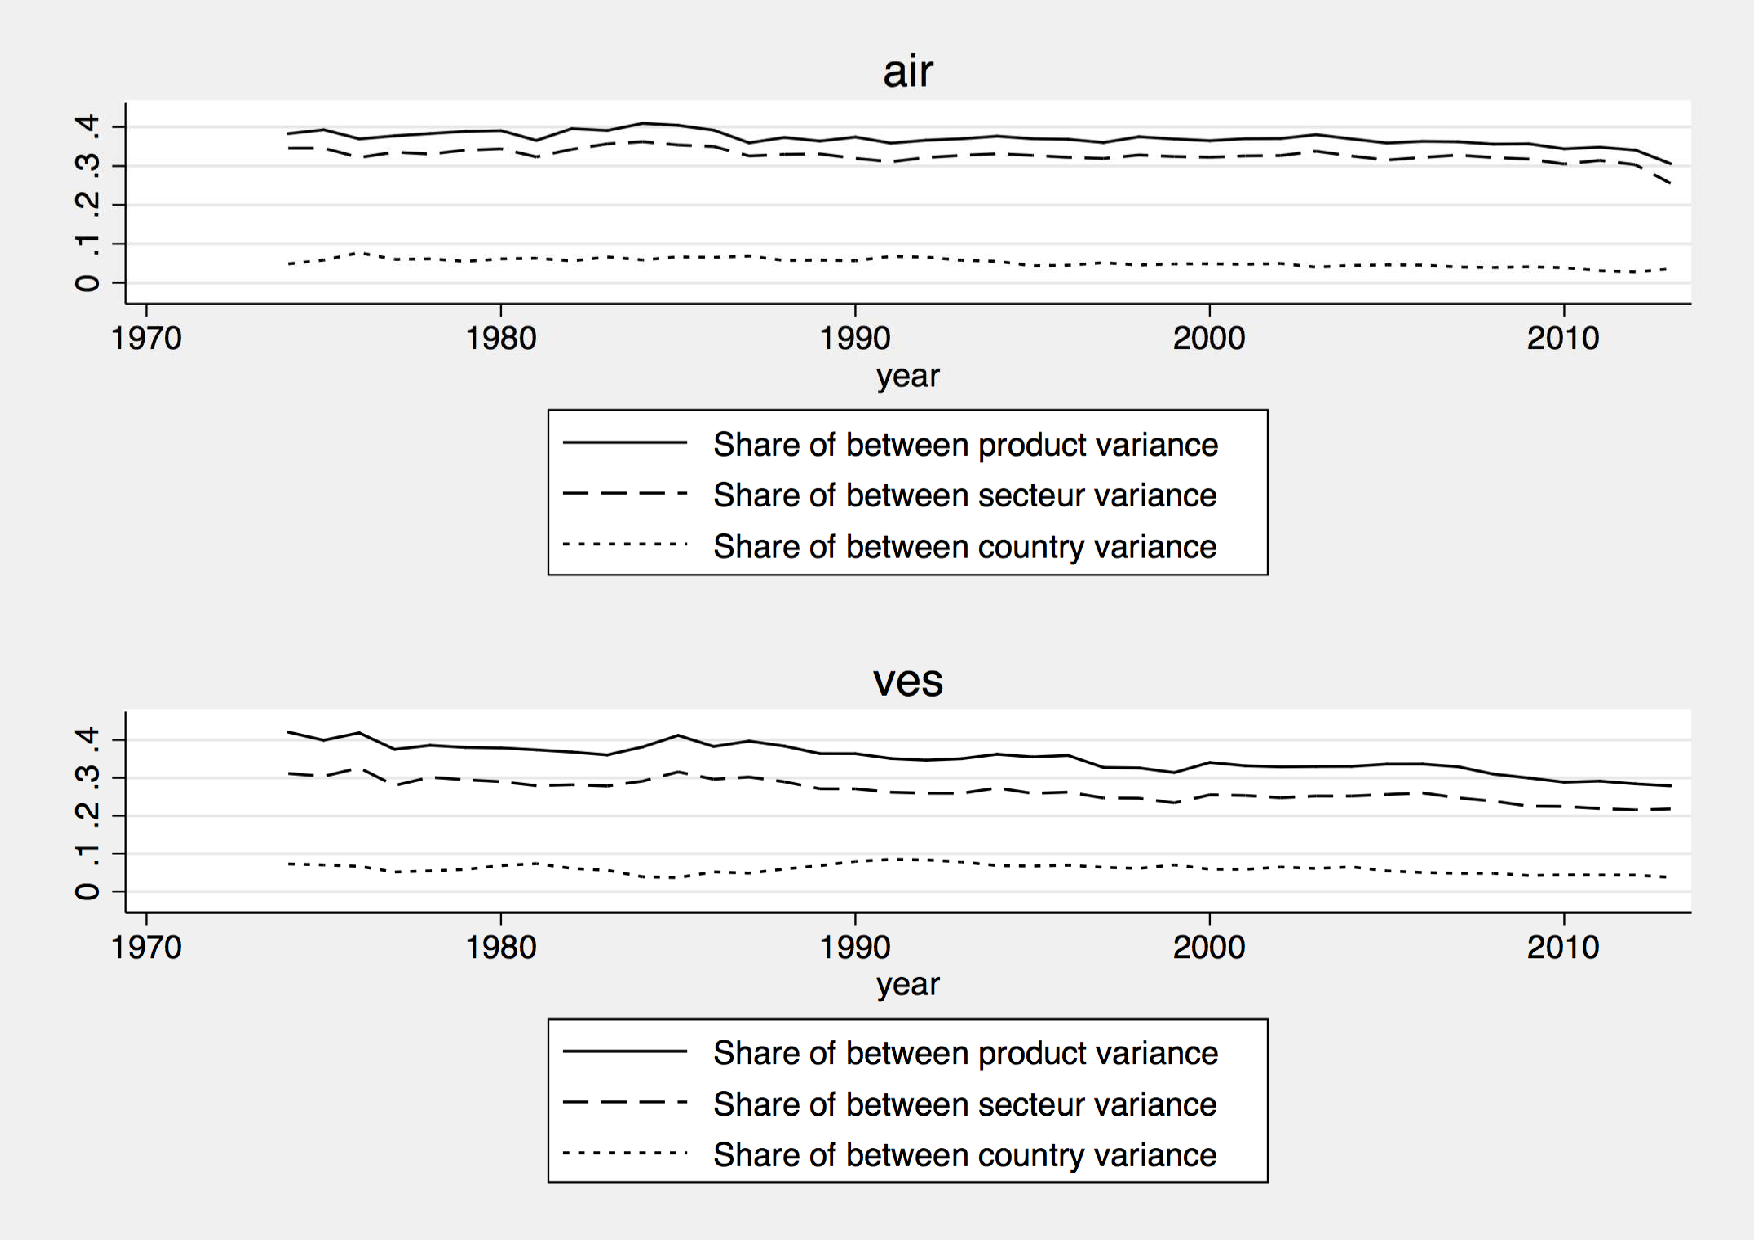
\includegraphics[width=10cm, height=7cm]{variance_decomposition.pdf}
%{\footnotesize {OECD data} }
\end{center}
\end{figure}


Two interesting results emerge from Figure \ref{fig:decomp_variance}.
First, the share of the cif-fas price gap variance that comes from the variance between products (5-digit level) is of the same magnitude of order as the variance between sectors at the 3-digit level.
Both account for between 30 and 40\% of the total variance in air transport, depending on the years considered.
This is also the case for vessel transport, even if the difference between the between-product variance share and the between-sector share is more pronounced (30\% for the between-sector vs 40\% for the between-product variance at the beginning of the period).
This provides an indirect robustness check to the degree of classification we have retained to estimate international transport costs.
Second, the variance of the cif-fas price gap that can be attributed to the product (or sector) dimension is much larger than the between-country variance.
This holds throughout the period and for both transport modes.
This suggests that what primarily matters in international transport costs is mostly attributable to the product \textit{per se}, rather than to the country where it comes from.
%JH: un peu too much, non ? "By extension, one can expect a limited role of distance and other country-related variables as determinants of transport costs."



\subsection{IV estimates: First stage \label{app:first_stage_IV}}

We report here the first-stage procedure and estimates underlying the IV estimates reported in section \ref{sec:results_decomposition}. We start by detailing the theoretical intuitions behind the first-stage equation. Afterwards, we report the estimates based on 5-digit-product-level data, before moving to the more disaggregate HS10 level for sensitivity checks.

\paragraph{First-stage equation.}

Our main instrumental variable for the fas price $\widetilde{p}_{ikt}$ is the share of tariff duties over the total value imported, at the product line. Tariffs may be considered as a (reasonably) exogenous source of variation for fas prices, i.e., uncorrelated with transport costs changes and mostly independent from firm- or sector-level dynamics. In this respect, considering the predicted part of the fas price related to tariff duties is likely to solve potential endogeneity biases. In other words, tariff shocks should eliminate from the fas price any endogenous component that might be related to transport costs. Note that this strategy has been regularly used in the related literature - see for example \citet{Caliendo_Parro_2015} or \citet{Lashkaripour-2017}.

Denoting as usual $i$ the origin country, $k$ the product at the 5 digit level, we assume that the fas price $\widetilde{p}_{ik}$ decomposes in two components, say $\bar{p}_{ik}$ the ``firm-specific'' price (related to its cost and pricing strategy) and $\tau^d_{ik}$ the tax duty (out of the firm's hands) according to :

\begin{equation}
\widetilde{p}_{ikt} = (1+\tau^d_{is(k)t})^\alpha \left(\bar{p}_{ikt}\right)^\beta \label{eq:link_fas_duty}
\end{equation}

\noindent with $s(k)$ the 3-digit classification as a function of the 5-digit product classification.

We first-differentiate this equation (between $t$ and $t-1$), with $\Delta $ the difference operator ($\Delta\widetilde{p}_{ikt} = \widetilde{p}_{ikt} - \widetilde{p}_{ikt-1}$ and so on):
\begin{eqnarray*}
&&\Delta \widetilde{p}_{ikt} = \beta \bar{p}_{ikt-1}^{\beta-1}(1+\tau^d_{is(k)t-1})\Delta \bar{p}_{ikt} + \alpha \bar{p}^\beta_{ikt-1} (1+\tau^d_{ikt-1})^{\alpha-1}\Delta \tau^d_{is(k)t}  \\
\Leftrightarrow &&\frac{\Delta \widetilde{p}_{ikt}}{\widetilde{p}_{ikt-1}} = \beta \frac{\Delta \bar{p}_{ikt}}{\widetilde{p}_{ikt-1}} \frac{(1+\tau^d_{is(k)t-1})^\alpha \bar{p}_{ikt-1}^\beta}{\bar{p}^\beta_{ikt-1}(1+\tau^d_{is(k)t-1})^\alpha} +\alpha \frac{\Delta \tau^d_{is(k)t-1}}{1+\tau_{is(k)t-1}^d}\frac{(1+\tau^d_{is(k)t-1})^\alpha \bar{p}_{ikt-1}^\beta}{\bar{p}^\beta_{ikt-1}(1+\tau^d_{is(k)t-1})^\alpha} \end{eqnarray*}

leading to:
\begin{equation}
\frac{\Delta \widetilde{p}_{ikt}}{\widetilde{p}_{ikt-1}} =  \beta \frac{\Delta \bar{p}_{ikt}}{\bar{p}_{ikt-1}} +\alpha\frac{\Delta \tau^d_{is(k)t}}{1+\tau_{ikt-1}^d} \label{eq:firststage_Deltalog}
\end{equation}

Equation (\ref{eq:firststage_Deltalog}) brings a first-stage regression model as follows:

$$\frac{\Delta \widetilde{p}_{ikt}}{\widetilde{p}_{ikt-1}} = \alpha \frac{\Delta \tau^d_{is(k)t}}{1+\tau_{is(k)t-1}^d} + \gamma_{i} +\gamma_{k}+\epsilon_{ik}$$

Or equivalently, taking logs:
$$\Delta \log \widetilde{p}_{ikt}= \alpha\frac{\Delta \tau^d_{is(k)t}}{1+\tau_{is(k)t-1}^d} +\gamma_{i} +\gamma_{k}+\epsilon_{ikt}$$


\noindent with the LHS being the growth rate of the fas price (between $t$ and $t-1$). $\frac{\Delta \tau^d_{is(k)t}}{1+\tau_{is(k)t-1}^d}$ is the change in the considered tariff rate, the second and third terms are fixed effects designed to capture changes in the ``firm-specific price'' $\bar{p}_{ik}$, $\epsilon_{ikt}$ being the residual. Note that, consistently with the second stage, the first stage will be estimated on a year-by-year basis, and will incorporate 3-digit-sector fixed effects. This implies to consider the following functional form of the first-stage equation:

\begin{equation}
\Delta \log \widetilde{p}_{ikt} = \alpha\frac{\Delta \tau^d_{is(k)t}}{1+\tau_{is(k)t-1}^d} +\gamma_{i} +\gamma_{s}+\epsilon_{ikt} \label{eq:firststage_Deltalog}
\end{equation}

or equivalently:

\begin{equation}
\log \widetilde{p}_{ikt} = \log \widetilde{p}_{ikt-1} + \alpha\frac{\Delta \tau^d_{is(k)t}}{1+\tau_{is(k)t-1}^d} +\gamma_{i} +\gamma_{s}+\epsilon_{ikt} \label{eq:firststage_Deltalog_bis}
\end{equation}

Finally, we allow for more flexibility in the empirical set-up, by allowing a variable degree of persistence in the fas price, i.e. by relieving the constraint of a unit parameter on $\log \widetilde{p}_{ikt-1}$:


\begin{equation}
\log \widetilde{p}_{ikt} = \beta\log \widetilde{p}_{ikt-1} + \alpha\frac{\Delta \tau^d_{is(k)t}}{1+\tau_{is(k)t-1}^d} +\gamma_{i} +\lambda_{s(k)}+\epsilon_{ikt} \label{eq:firststage_final}
\end{equation}

Note that in such a formulation, $\log \widetilde{p}_{ikt-1}$ appears as a second instrument for $\log \widetilde{p}_{ikt}$. The $\alpha$ parameter should fall between $-1$ and $0$, and has a direct theoretical interpretation in terms of ``pricing-to-market'' behavior of firms. $\alpha = 0$ corresponds to the case where the considered sector is made of firms not adjusting their fas price to the change in tariff, that would cancel out the influence of the tariff change on the price paid by the US consumers; this rather corresponds to small firms which do not have enough market power to manipulate their prices following changes in international competition. $\alpha = -1$ is the other polar case: the sector here displays full pricing-to-market, because it involves large firms fully compensating the tariff change through their margin (see \citealp{Berman_Martin_Mayer_2012}).
In-between, $\alpha$ $\in$ $]-1,0[$ corresponds to some variable degree of``pricing-to-market'' in the sector, characterized by firms offsetting partly the impact of the tariff change on the fas price by adjusting the producer price in the opposite direction of the tariff change.

As already mentioned, consistently with the cross-section analysis adopted by now, the first-stage equation is estimated on a yearly basis, and implements 3-digit sector fixed effects ($\lambda_{is(k)}$ ). We then replace the observed series of fas prices in the right-hand side of Equation (\ref{eq:model_IetA}) by the predicted fas prices produced by Equation (\ref{eq:firststage_final}). We now report results based on our main database at the SITC 5-digit level, before replicating the exercise on HS10 digit level, consistently with one major robustness implemented in the paper.

\paragraph{First-stage estimates based on SITC5 data.}

Here we run Equation (\ref{eq:firststage_final}) on our standard dataset, based on SITC-5 data. Consistently, we will use as instrument 5-digit product-specific tariff rates, as well as the one-year-lagged fas price. Table \ref{tab: FS_sitc5} reports summary results of these first stage regressions, while Figure \ref{fig: FS_IV_SITC5} displays year estimates of $\beta$ and $\alpha$ parameters, together with 5\% confidence bands:


\begin{table}[htbp]\centering
\caption{Summary Results for First-Stage Regressions\label{tab: FS_sitc5}}
\begin{tabular} {@{} l r r r r r r r @{}} \\ \hline
\textbf{variable } & \textbf{Mean} & \textbf{1\textsuperscript{st} Quart.} & \textbf{Median} & \textbf{3\textsuperscript{rd} Quart.} & \textbf{ S.D.} & \textbf{Min} & \textbf{Max} \\
\hline
 $\log \widetilde{p}_{ikt-1}$ ($\widehat{\beta}$)&     0.7484 &     0.7400 &     0.7551 &     0.7663 &     0.0248 &     0.6616 &     0.7788 \\
 % sd_lag~b  &     0.0051 &     0.0040 &     0.0045 &     0.0065 &     0.0015 &     0.0037 &     0.0093 \\
Student t$_{\widehat{\beta}}$  &   157.07 &   113.24 &   168.82 &   191.15 &    41.23 &    82.88 &   208.23 \\
$\frac{\Delta \tau^d_{is(k)t}}{1+\tau_{is(k)t-1}^d}$ ($\widehat{\alpha}$)  &    -0.6324 &    -0.8858 &    -0.6079 &    -0.3639 &     0.3962 &    -1.8353 &     0.0534 \\
 %sd_tar~f  &     0.2216 &     0.2149 &     0.2363 &     0.2599 &     0.0681 &     0.0031 &     0.3399 \\
 Student t$_{\widehat{\alpha}}$  &    -2.8178 &    -3.7575 &    -2.5741 &    -1.8099 &     1.6808 &    -7.3086 &     0.2280 \\
 %F_stat  &   1.32e+04 &  6436.5362 &   1.43e+04 &   1.83e+04 &  6174.8488 &  3452.2548 &   2.17e+04 \\
  F-statistic $\frac{\Delta \tau^d_{is(k)t}}{1+\tau_{is(k)t-1}^d}$  &    10.7023 &     3.2757 &     6.6260 &    14.1188 &    11.4529 &     0.0008 &    53.4159 \\
  %adj_r_~e  &     0.7843 &     0.7809 &     0.7858 &     0.7899 &     0.0105 &     0.7438 &     0.8075 \\
%  $R^2$ within&     0.5610 &     0.5424 &     0.5738 &     0.5846 &     0.0339 &     0.4373 &     0.5972 \\
\hline
%\multicolumn{8}{@{}l}{\footnotesize{\emph{Source:} C:\Users\coadministrateur\Dropbox\Papier_Lise_Guillaume\private\revision_JOEG\IV_rev/results/IV_referee1_yearly/FS_parameters_both_yearly_prod5_sect3.dta}}
\end{tabular}
\end{table}




\begin{figure}[htbp]
\caption{Yearly estimates of $\alpha$ and $\beta$ - SITC5}\label{fig: FS_IV_SITC5}
\begin{center}
\begin{tabular}{cc}
%{\small (a) $\beta$} & {\small (b) $\alpha$}\\
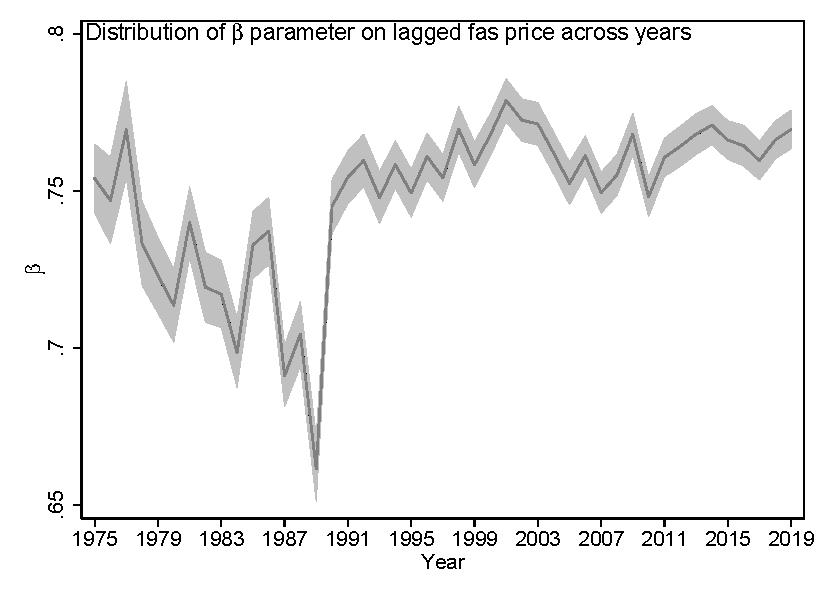
\includegraphics[width=3.2in, height=3.2in,keepaspectratio]{beta_lag_SITC5.pdf}
& 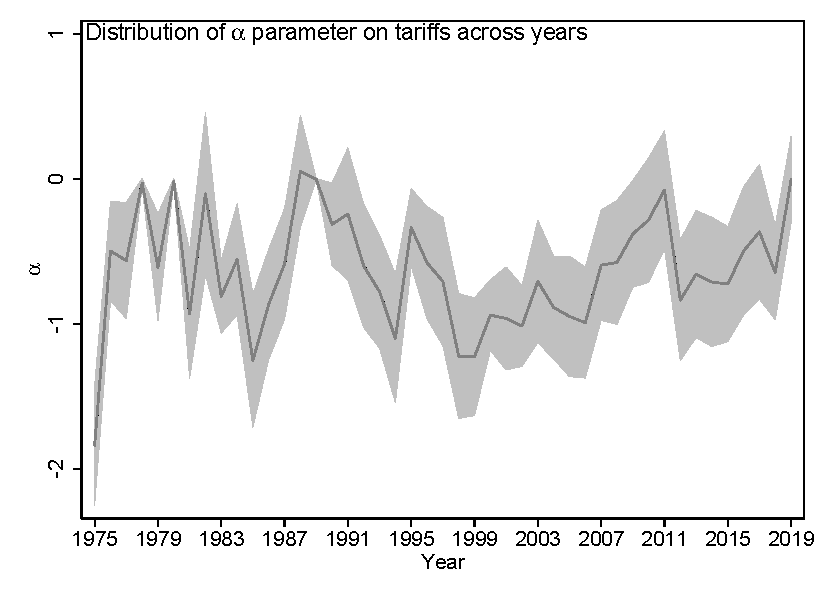
\includegraphics[width=3.2in,height=3.2in,keepaspectratio]{alpha_tariff_SITC5.pdf} \\
\end{tabular}
\end{center}
\end{figure}

%Staiger and Stock (1997) formalized the definition of “weak instruments” and most researchers seem to have concluded (incorrectly) from that work (orhearsay) that if the F-statistic on the excluded instruments in the first stage is greater than 10, one need worry no further about weak instruments.

%\newpage

Table \ref{tab: FS_sitc5} suggests that custom duties variations are a satisfactory predictor of fas prices $\widetilde{p}_{ik}$, with strong significance and the correct, negative sign. The lagged fas price $\log \widetilde{p}_{ikt-1}$ displays also the expected positive sign: with a $\beta$ parameter around 0.75 on average, fas prices exhibit substantial persistence. The F-statistic on the excluded instrument ($\frac{\Delta \tau^d_{is(k)t}}{1+\tau_{is(k)t-1}^d}$ ($\widehat{\alpha}$)) is on average above 10, the ``rule-of-thumb'' threshold value recommended by \cite{staiger_stock} as a test for weak instrumentation. In addition, Figure \ref{fig: FS_IV_SITC5} shows that most values of the $\alpha$ parameter stand between 0 and -1, as expected, except in a very small number of occasions, corresponding to abrupt fluctuations in oil prices. This is typically the case in 1975, with $\alpha$=-1.83. All in all, these estimates make us confident in the validity of our instrumentation strategy.



\paragraph{First-stage estimates based on HS10 data.}

Here we replicate our first-stage estimations using HS10 data, available between 2002 and 2019. In addition to one-year-lagged fas price, we use this time HS10-digit product-specific tariff duties. Table \ref{tab: FS_HS10} reports summary results of these first-stage regressions, while Figure \ref{fig: FS_IV_HS10} presents yearly estimates of $\beta$ and $\alpha$ parameters, together with 5\% confidence bands:


\begin{table}[htbp]\centering
\caption{Summary Results for First-Stage Regressions\label{tab: FS_HS10}}
\begin{tabular} {@{} l r r r r r r r @{}} \\ \hline
\textbf{variable } & \textbf{Mean} & \textbf{1\textsuperscript{st} Quart.} & \textbf{Median} & \textbf{3\textsuperscript{rd} Quart.} & \textbf{ S.D.} & \textbf{Min} & \textbf{Max} \\
\hline
$\log \widetilde{p}_{ikt-1}$ ($\widehat{\beta}$) &     0.7496 &     0.7453 &     0.7504 &     0.7539 &     0.0055 &     0.7385 &     0.7578 \\
 % sd_lag~t  &     0.0020 &     0.0020 &     0.0020 &     0.0021 &     0.0001 &     0.0019 &     0.0021 \\
Student t$_{\widehat{\beta}}$  &   369.81 &   361.19 &   366.34 &   376.77 &    12.91 &   352.61 &   395.33 \\
$\frac{\Delta \tau^d_{is(k)t}}{1+\tau_{is(k)t-1}^d}$ ($\widehat{\alpha}$)  &    -0.3612 &    -0.5636 &    -0.4175 &    -0.1918 &     0.3393 &    -0.9258 &     0.3448 \\
%  sd_tar~f  &     0.1511 &     0.1451 &     0.1618 &     0.1702 &     0.0325 &     0.0728 &     0.2011 \\
 Student t$_{\widehat{\alpha}}$   &    -2.2505 &    -3.3518 &    -2.5489 &    -1.3144 &     2.7027 &    -7.9494 &     4.7359 \\
  %  F_stat  &   6.85e+04 &   6.52e+04 &   6.71e+04 &   7.10e+04 &  4854.7592 &   6.22e+04 &   7.83e+04 \\
 F-statistic $\frac{\Delta \tau^d_{is(k)t}}{1+\tau_{is(k)t-1}^d}$ &    11.9399 &     1.7974 &     9.0342 &    14.8620 &    15.1916 &     0.8415 &    63.1932 \\
%  adj_r_~e  &     0.7697 &     0.7660 &     0.7691 &     0.7725 &     0.0068 &     0.7550 &     0.7826 \\
%  r_squa~n  &     0.5617 &     0.5591 &     0.5624 &     0.5661 &     0.0057 &     0.5505 &     0.5693 \\
\hline
%\multicolumn{8}{@{}l}{\footnotesize{\emph{Source:} C:\Users\coadministrateur\Dropbox\Papier_Lise_Guillaume\private\revision_JOEG\IV_rev/results/IV_referee1_yearly/FS_parameters_both_yearly_prod5_sect3.dta}}
\end{tabular}
\end{table}

\begin{figure}[htbp]
\caption{Yearly estimates of $\alpha$ and $\beta$ - HS10}\label{fig: FS_IV_HS10}
\begin{center}
\begin{tabular}{cc}
%{\small (a) $\beta$} & {\small (b) $\alpha$}\\
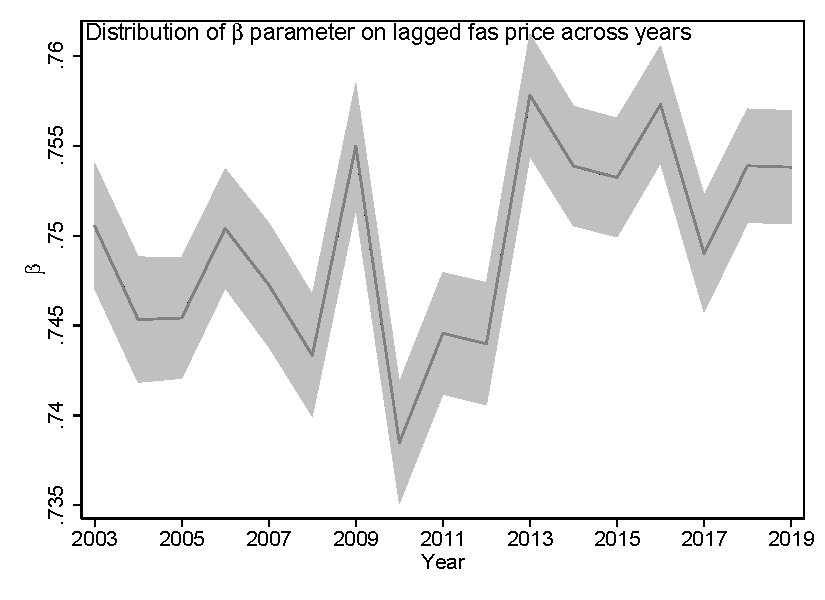
\includegraphics[width=3.2in, height=3.2in,keepaspectratio]{beta_lag_HS10.pdf}
& 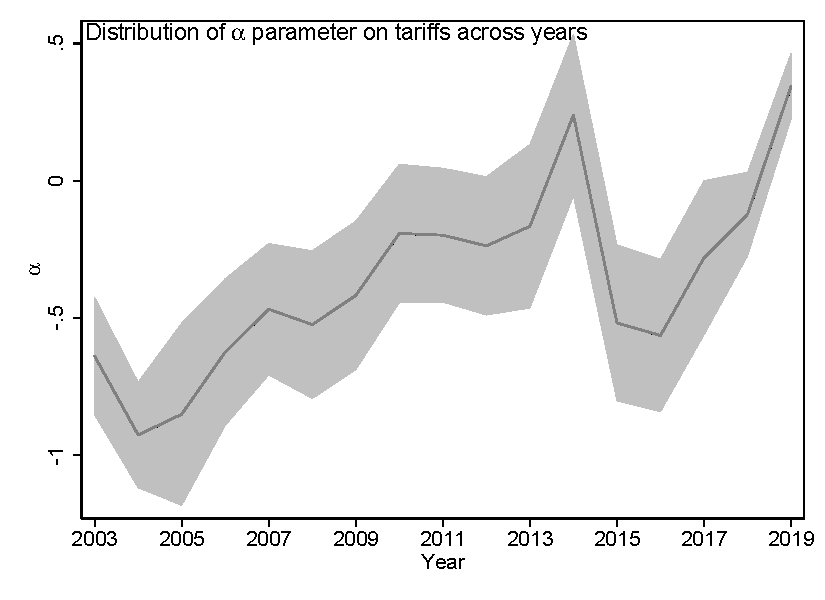
\includegraphics[width=3.2in,height=3.2in,keepaspectratio]{alpha_tariff_HS10.pdf} \\
\end{tabular}
\end{center}
\end{figure}

Results are qualitatively very similar to those reported on the longer-time-span, more-aggregated-SITC5 dataset previously reported. The F-statistic on the excluded instrument ($\frac{\Delta \tau^d_{is(k)t}}{1+\tau_{is(k)t-1}^d}$ ($\widehat{\alpha}$)) is on average close to 12, slightly higher than in our benchmark. As previously, Figure \ref{fig: FS_IV_HS10} shows that most values of the $\alpha$ parameter stand between 0 and -1, as expected, except in a few years which seem again to coincide with significant fluctuations in oil prices. Interestingly, the value of the $\alpha$ parameter is on average -0.36, lower than in our benchmark on SITC5 data. At this highly disaggregated level, pricing-to-market behavior seems less strong, indicating that the average firm is smaller than its average SITC5 counterpart. In addition, this average value is almost identical to the one found by \citet{Fontagne_Martin_Orefice2018} on French HS6 data between 1995 and 2010 (see the first-stage coefficients in their Table 6), or by \citet{Bussiere2013} on country-level data between 1980 and 2006. In any case, this strengthens our confidence in the validity of our estimation strategy.

\clearpage
\setcounter{table}{0}
\setcounter{figure}{0}
\renewcommand{\thefigure}{C.\arabic{figure}}
\renewcommand{\thetable}{C.\arabic{table}}

\section{Estimation at the 4-digit level \label{app:4digit}}

In this section, we report the estimation results when we retain the 4-digit classification level ($s$=4-digit).

\subsection{Transport cost estimates}


Tables \ref{tab:result_air_rob} and \ref{tab:result_ves_rob} report the estimates of both models (with and without additive costs) in air and ocean transport respectively.

\begin{table}[htbp]
  \centering
  \caption{Air: Transport costs estimates, selected years, 4-digit level}
\begin{center}
  \footnotesize{
    \begin{tabular}{l|cccccc}
   \hline\hline
Year & 1974  & 1981  & 1989  & 2001  & 2009  & 2013 \\ \hline
\multicolumn{7}{l}{\textbf{Model (a) - With only Ad-Valorem TC} ($\widehat{\tau}^{ice}-1$, in \%) }  \\
\hline
Mean  & 6.6 & 5.8 & 5.2 & 3.3 & 3.7 & 3.2 \\
Median & 5.2 & 4.4 & 4.1 & 2.1 & 2.7 & 2.6 \\
%Standard Error & 0.056 & 0.054 & 0.046 & \multicolumn{1}{c}{0.040} & \multicolumn{1}{c}{0.036} & \multicolumn{1}{c}{0.025}  \\
\hline
\multicolumn{7}{l}{\textbf{Model (b) - With Additive \& Ad-Valorem TC}}  \\ \hline
\multicolumn{7}{l}{\textit{Ad-valorem term }($\widehat{\tau}^{adv}-1$, in \%) }   \\ \hline
Mean  & 3.5 & 2.6 & 3.1 & 1.5 & 2.1 & 1.6  \\
Median & 2.5 & 1.7 & 1.9 & 1.0 & 1.7 & 1.4  \\
%Standard Error & 0.036 & 0.028 & 0.030 & \multicolumn{1}{c}{0.021} & \multicolumn{1}{c}{0.024} & \multicolumn{1}{c}{0.015}  \\
\hline
\multicolumn{7}{l}{\textit{Additive term} ($\widehat{t}/\widetilde{p}$), in \%}    \\ \hline
Mean  & 2.6 & 2.1 & 1.7 & 1.2 &1.2 & 1.0 \\
Median & 1.2 & 0.6 & 0.6 & 0.5 & 0.4 & 0.4  \\
%Standard Error & 0.039 & 0.042 & 0.033 & \multicolumn{1}{c}{0.027} & \multicolumn{1}{c}{0.029} & \multicolumn{1}{c}{0.019} \\
\hline
\# observations & 14944 & 16844 & 25307 & \multicolumn{1}{c}{35005} & \multicolumn{1}{c}{38475} & \multicolumn{1}{c}{39460}  \\
\hline\hline
\multicolumn{7}{l}{\parbox[l]{11cm}{ \vspace{7pt}\scriptsize{Notes: TC = Transport Costs.
Statistics are obtained weighting each observation by its share in trade (mode-dependent).
Additive term expressed in fraction of fas price.}}}
\end{tabular}%
}
\end{center}
  \label{tab:result_air_rob}
\end{table}%


\begin{table}[htbp]
  \centering
\caption{Vessel: Transport costs estimates, selected years, 4-digit level}
\begin{center}
  \footnotesize{
    \begin{tabular}{l|cccccc}
   \hline\hline
Year & 1974  & 1981  & 1989  & 2001  & 2009  & 2013 \\
\hline
\multicolumn{7}{l}{\textbf{Model (a) - With only Ad-Valorem TC} ($\widehat{\tau}^{ice}-1$, in \%)} \\
\hline
Mean  & 9.8 & 6.1 & 5.8 & 5.1 & 4.2 & 3.6  \\
Median & 9.4 & 5.1 & 4.8 & 4.5 & 3.8 & 3.1 \\
%Standard Error & 0.060 & 0.038 & \multicolumn{1}{c}{0.036} & \multicolumn{1}{c}{0.030} & \multicolumn{1}{c}{0.023} & \multicolumn{1}{c}{0.020} \\
\hline
\multicolumn{7}{l}{\textbf{Model (b) - With Additive \& Ad-Valorem TC} }\\ \hline
\multicolumn{7}{l}{\textit{Ad-valorem term} ($\widehat{\tau}^{adv}-1$, in \%) }   \\ \hline
Mean  & 5.4 & 3.4 & 2.8 & 2.8 & 2.4 & 2.1  \\
Median & 4.9 & 3.0 & 2.4 & 2.5 & 2.6 & 1.8 \\
%Standard Error & 0.043 & 0.026 & \multicolumn{1}{c}{0.025} & \multicolumn{1}{c}{0.021} & \multicolumn{1}{c}{0.016} & \multicolumn{1}{c}{0.013}  \\
\hline
\multicolumn{7}{l}{\textit{Additive term} ($\widehat{t}^{add}/\widetilde{p}$, in \%) }   \\ \hline
Mean  & 4.6 & 2.6 & 3.1 & 2.4 & 2.1 & 1.5  \\
Median & 2.9 & 1.3 & 1.9 & 1.5 & 1.3 & 0.8 \\
%Standard Error & 0.068 & 0.044 & \multicolumn{1}{c}{0.037} & \multicolumn{1}{c}{0.035} & \multicolumn{1}{c}{0.031} & \multicolumn{1}{c}{0.023} \\
\hline
\# observations & 19196 & 17916 & \multicolumn{1}{c}{29387} & \multicolumn{1}{c}{36677} & \multicolumn{1}{c}{37643} & \multicolumn{1}{c}{38820} \\
\hline\hline
\multicolumn{7}{l}{\parbox[l]{11cm}{ \vspace{7pt}\scriptsize{Notes: TC = Transport Costs.
Statistics are obtained weighting each observation by its share in trade (mode-dependent).
Additive term expressed in fraction of fas price.}}}
\end{tabular}%
}
\end{center}
\label{tab:result_ves_rob}%
\end{table}%

\subsection{Goodness-of-fit tests at the 4-digit level}

We now report the goodness-of-fit exercise (conducted by transport mode) at the 4-digit product classification level (for the selected years).
The results are reported in Tables \ref{tab:good_fit_air_rob} (for air) and \ref{tab:good_fit_ves_rob} (for vessel).
\begin{table}[htbp]
  \centering
  \caption{Air: Measures of goodness of fit, 4-digit level}
\begin{center}
\label{tab:good_fit_air_rob}%
%\vspace{0.5cm}
%\scalebox{0.97}{
  \footnotesize{
\begin{tabular}{l|cccccc}
\hline
\hline
      & \multicolumn{6}{c}{Year}              \\
      & \multicolumn{1}{c}{1974} & \multicolumn{1}{c}{1981} & \multicolumn{1}{c}{1989} & \multicolumn{1}{c}{2001} & \multicolumn{1}{c}{2009} & \multicolumn{1}{c}{2013}  \\
\hline
\multicolumn{7}{l}{\textbf{R$^2$}}      \\ \hline
Model (a)& \multicolumn{1}{c}{0.48} & \multicolumn{1}{c}{0.49} & \multicolumn{1}{c}{0.50} & \multicolumn{1}{c}{0.50} & \multicolumn{1}{c}{0.45} & \multicolumn{1}{c}{0.35} \\
Model (b) & \multicolumn{1}{c}{0.63} & \multicolumn{1}{c}{0.66} & \multicolumn{1}{c}{0.65} & \multicolumn{1}{c}{0.66} & \multicolumn{1}{c}{0.54} & \multicolumn{1}{c}{0.45} \\ \hline
\multicolumn{7}{l}{\textbf{SER} }  \\ \hline
Model (a)& \multicolumn{1}{c}{0.8} & \multicolumn{1}{c}{0.9} & \multicolumn{1}{c}{0.83} &   0.87    & \multicolumn{1}{c}{0.88} & \multicolumn{1}{c}{0.93}  \\
Model (b) & \multicolumn{1}{c}{0.67} & \multicolumn{1}{c}{0.74} & \multicolumn{1}{c}{0.69} &  0.80     & \multicolumn{1}{c}{0.80} & \multicolumn{1}{c}{0.86}  \\
\multicolumn{7}{l}{\textbf{Log-likelihood} } \\ \hline
Model (a) & \multicolumn{1}{c}{-17505.6} & \multicolumn{1}{c}{-21813.5} & \multicolumn{1}{c}{-30960.6} & \multicolumn{1}{c}{-44067.6} & \multicolumn{1}{c}{-49375.6} & \multicolumn{1}{c}{-53197.9}  \\
Model (b) & \multicolumn{1}{c}{-14895.8} & \multicolumn{1}{c}{-18589.9} & \multicolumn{1}{c}{-26553.5} & \multicolumn{1}{c}{-37297.9} & \multicolumn{1}{c}{-45747.6} & \multicolumn{1}{c}{-49899.1}  \\ \hline
\multicolumn{7}{l}{\textbf{AIC criteria} }  \\ \hline
Model (a)& \multicolumn{1}{c}{36243.1} & \multicolumn{1}{c}{44966.9} & \multicolumn{1}{c}{63417.1} & \multicolumn{1}{c}{89747.2} & \multicolumn{1}{c}{100317.13} & \multicolumn{1}{c}{107963.7} \\
Model (b) & \multicolumn{1}{c}{31873.6} & \multicolumn{1}{c}{39495.8} & \multicolumn{1}{c}{55777.1} & \multicolumn{1}{c}{77439.9} & \multicolumn{1}{c}{94059.1} & \multicolumn{1}{c}{102224.3}  \\ \hline
\multicolumn{7}{l}{\textbf{Test LL} }    \\ \hline
2$\times$(ll(UR) -ll(R)) & \multicolumn{1}{c}{5219.5} & \multicolumn{1}{c}{6447.1} & \multicolumn{1}{c}{8814.1} & \multicolumn{1}{c}{13539.4} & \multicolumn{1}{c}{7256.0} & \multicolumn{1}{c}{6597.5}  \\
\# restrictions  & \multicolumn{1}{c}{640} & \multicolumn{1}{c}{698} & \multicolumn{1}{c}{778} & \multicolumn{1}{c}{833} & \multicolumn{1}{c}{824} & \multicolumn{1}{c}{818}  \\
p-value & \multicolumn{1}{c}{0.00} & \multicolumn{1}{c}{0.000} & \multicolumn{1}{c}{0.00} & \multicolumn{1}{c}{0.00} & \multicolumn{1}{c}{0.00} & \multicolumn{1}{c}{0.000} \\
\hline\hline
\multicolumn{7}{l}{\parbox[l]{13cm}{ \vspace{7pt}\scriptsize{Notes: Model (a) = with only ad-valorem transport costs.
Model (b) = with additive \& ad-valorem
transport costs.
$R^{2}$ between the log of predicted ratio and the log of the observed ratio.
The number \# of restrictions is equal to the number of parameters estimated, i.e. the number of partner countries plus the number of products.}}}
\end{tabular}%
}
\end{center}
\end{table}%


\begin{table}[htbp]
  \centering
  \caption{Vessel: Measures of goodness of fit, 4-digit level}
\begin{center}
\label{tab:good_fit_ves_rob}%
  \footnotesize{
\begin{tabular}{l|cccccc}
\hline
\hline
      & \multicolumn{6}{c}{Year}                   \\
      & \multicolumn{1}{c}{1974} & \multicolumn{1}{c}{1981} & \multicolumn{1}{c}{1989} & \multicolumn{1}{c}{2001} & \multicolumn{1}{c}{2009} & \multicolumn{1}{c}{2013}  \\ \hline
\multicolumn{7}{l}{\textbf{R$^{2}$}} \\ \hline
Term I only & 0.50  & 0.45  & \multicolumn{1}{c}{0.47} & \multicolumn{1}{c}{0.41} & \multicolumn{1}{c}{0.37} & \multicolumn{1}{c}{0.35} \\
Terms A \& I & 0.66  & 0.62  & \multicolumn{1}{c}{0.62} & \multicolumn{1}{c}{0.58} & \multicolumn{1}{c}{0.51} & \multicolumn{1}{c}{0.46} \\ \hline
\multicolumn{7}{l}{\textbf{SER} }\\ \hline
Model (a) &    0.58   &   0.64    & \multicolumn{1}{c}{0.61} & \multicolumn{1}{c}{0.0.72} & \multicolumn{1}{c}{0.79} & \multicolumn{1}{c}{0.82} \\
Model (b) &   0.48    &    0.53   & \multicolumn{1}{c}{0.51} & \multicolumn{1}{c}{0.61} & \multicolumn{1}{c}{0.69} & \multicolumn{1}{c}{0.75} \\ \hline
\multicolumn{7}{l}{\textbf{Log-likelihood} } \\ \hline
Model (a)& -16460.1 & -16951.6 & \multicolumn{1}{c}{-26771.4} & \multicolumn{1}{c}{-39008.3} & \multicolumn{1}{c}{-43888.9} & \multicolumn{1}{c}{-47161.6} \\
Model (b) & -12743.65 & -13546.9 & \multicolumn{1}{c}{-21752.8} & \multicolumn{1}{c}{-33281.0} & \multicolumn{1}{c}{-39078.9} & \multicolumn{1}{c}{-43399.2}  \\ \hline
\multicolumn{7}{l}{\textbf{AIC criteria} } \\ \hline
Model (a) & 34464.2 & 35491.2 & \multicolumn{1}{c}{55272.9} & \multicolumn{1}{c}{79800.7} & \multicolumn{1}{c}{89459.8} & \multicolumn{1}{c}{95987.2}\\
Model (b) & 28271.3 & 29877.8 & \multicolumn{1}{c}{46595.6} & \multicolumn{1}{c}{69743.9} & \multicolumn{1}{c}{81155.7} & \multicolumn{1}{c}{89692.4} \\ \hline
\multicolumn{7}{l}{\textbf{Test LL}} \\ \hline
2$\times$(ll(UR) -ll(R)) & 12385.80 & 11226.8 & \multicolumn{1}{c}{17354.7} & \multicolumn{1}{c}{20113.5} & \multicolumn{1}{c}{16608.2} & \multicolumn{1}{c}{12589.6} \\
\# restrictions  & 797   & 814   & \multicolumn{1}{c}{881} & \multicolumn{1}{c}{910} & \multicolumn{1}{c}{886} & \multicolumn{1}{c}{874} \\
p-value & 0.000 & 0.000 & \multicolumn{1}{c}{0.000} & \multicolumn{1}{c}{0.000} & \multicolumn{1}{c}{0.000} & \multicolumn{1}{c}{0.000} \\
\hline\hline
\multicolumn{7}{l}{\parbox[l]{13cm}{ \vspace{7pt}\scriptsize{Notes: Model (a) = with only ad-valorem transport costs.
Model (b) = with additive \& ad-valorem
transport costs.
$R^{2}$ between the log of predicted ratio and the log of the observed ratio.
The number \# of restrictions is equal to the number of parameters estimated, i.e. the number of partner countries plus the number of products.}}}
\end{tabular}%
}
\end{center}
\end{table}%

\newpage


\clearpage
\setcounter{table}{0}
\setcounter{figure}{0}
\renewcommand{\thefigure}{D.\arabic{figure}}
\renewcommand{\thetable}{D.\arabic{table}}

\section{Eliminating the composition effects: more details \label{app:comp-effects}}

In this section, we explain in more detail the method employed to eliminate the country and product dimensions of the estimated transport cost.

\subsection{More on our methodology}


\subsubsection{Estimation method for each additive and multiplicative component}

We begin by describing the estimation method to extract the fitted and unfitted series for both the additive and the multiplicative components, before turning to the `total costs'' series.
\smallskip

\paragraph{Obtaining the ``pure'' transport costs component series} - The empirical strategy to find the fitted transport cost measure (i.e. extracting from trade composition effect) can be described as a two-stage process.
First, we decompose the estimated measure in the three product/country/time dimensions, using fixed effects. In plain words, we measure how these costs have changed over time by blocking the composition of trade flows by product and country partners to the one observed in 1974 (the beginning of our sample).\smallskip

For the estimated ad-valorem component, we estimate the following equation:
\begin{eqnarray}
\ln(\widehat{\tau}_{ikt}-1)&=&\delta +\underbrace{\sum_{i \neq \text{ARG}}\alpha_i.\mathbbm{1}_i}_{(a)} + \underbrace{\sum_{s(k)\neq \text{011}}\beta_{s(k)}.\mathbbm{1}_{s(k)}}_{(b)} + \underbrace{\sum_{t \neq 1974}\gamma_t.\mathbbm{1}_t}_{(c)}+\epsilon_{ikt} \label{eq:compeffects_mult}
\end{eqnarray}

\noindent where $\mathbbm{1}_i$ and $\mathbbm{1}_{s(k)}$ represent country and sector fixed effects.\footnote{Throughout the exercise, we consider Argentina, the sector 011 and the first year of our dataset 1974, as references for the country, product and year dummies.}  Equation (\ref{eq:compeffects_mult}) is estimated using OLS, with a weighting scheme based on the value of each flow in the total value of flows for the relevant year.

In this exercise, we are interested in isolating the change in the time dimension of each transport cost component. This constitutes the second stage of our procedure. Based on Equation (\ref{eq:compeffects_mult}), we deduce after estimation that:

\[\left\{
  \begin{array}{lcl}
  \text{For the year 1974:} &&  \widehat{\tau}_{is74} -1 = \exp(\delta +\alpha_i+\beta_s), \\
  \text{For any year }t> 1974:&& \widehat{\tau}_{ist} -1 = \exp(\delta +\alpha_i+\beta_s)\times \exp(\gamma_t) \\
  \end{array}
\right.\]

From this, we obtain the following recursive link: $\widehat{\tau}_{ist} -1 = (\widehat{\tau}_{is74}-1)\exp(\gamma_t)$. Given the constraint $\tau>1$, we rewrite to get the percentage change between year 1974 and any year $t>1974$:
\begin{equation*}
\Gamma_{ist} = 100.\frac{\widehat{\tau}_{ist}-1}{\widehat{\tau}_{is74}-1} = 100.\frac{(\widehat{\tau}_{is74}-1)\exp(\gamma_t)}{\widehat{\tau}_{is74}} = 100\exp(\gamma_t)
\end{equation*}

As such, the index of transport costs in year $t$ (relative to the reference year 1974) $\Gamma_{ist} $  only depends on the cost observed in 1974 and the time trend. Note that it is independent of the product-origin country pair, such that we can rewrite:
\begin{equation}
 \Gamma^{adv}_t= 100\exp(\gamma^{adv}_t)  \label{eq:tcadv_compoeffect}
\end{equation}

\noindent where the subscript $^{adv}$ clarifies that this time fixed effect is specific to the ad-valorem component. \medskip

\textbf{REPRENDRE AVEC GUILLAUME. }

%At this stage though, it remains specific to a product-origin country pair.
%Next step is to build the index $\Gamma^{adv}_t$ such that:
%\begin{equation}
% \Gamma^{adv}_t= 100\frac {\bar{\tau}_{1974}.\exp(\gamma_t)} {\bar{\tau}_{19741}  \label{eq:tcadv_compoeffect}
%\end{equation}
%\noindent that is, Equation (\ref{eq:comp_effects_adv}) with $\bar{\tau}_{1974} = \exp(\delta + \sum_i \alpha_i + \sum_k \beta_k$) the mean (ad-valorem) transport cost in 1974.

\textbf{STOP HERE}

As for the additive component, given that the sector fixed effect and the country fixed effect are additive rather than multiplicative by construction, we estimate the following equation using non-linear least squares:\footnote{For sake of notational simplicity, we do not distinguish the coefficients associated with the fixed effects between Equations (\ref{eq:compeffects_mult}) and (\ref{eq:compeffects_add}), even if they are specific to the type of transport costs considered (e.g. the series of $\gamma_t$ differs from one estimation to the other).
Note that we apply the same weighting scheme as for the OLS regression (based on the relative value of the flow).}

%, based on the additive cost series $\widehat{t}_{ikt}$ previously obtained:
\begin{eqnarray}
\ln(\widehat{t}_{ikt})&=&\ln\left( \delta + \underbrace{\sum_{i \neq \text{ARG}}  \alpha_i.\mathbbm{1}_i}_{(a)}+\underbrace{\sum_{s(k)}\beta_{s(k)}.\mathbbm{1}_{s(k)}}_{(b)}\right) + \underbrace{\sum_{t \neq 1974}\gamma_t.\mathbbm{1}_t}_{(c)}+\epsilon_{ikt} \label{eq:compeffects_add}
\end{eqnarray}


As displayed in Equations (\ref{eq:compeffects_mult}) and (\ref{eq:compeffects_add}), we decompose the estimated transport cost component in three elements: the country dimension (Term (a)), the product dimension (Term (b)) and the pure transport costs time trend (Term (c)).
Note that Equations (\ref{eq:compeffects_mult}) and (\ref{eq:compeffects_add}) preserve our specification of the ad-valorem and additive costs of Equations (\ref{eq:ad-valorem}) and (\ref{eq:add}), as we consider that the iceberg cost is the product of the country of origin and the goods dimension, while the additive cost is the sum of the two dimensions.
Both equations are estimated by transport mode.\smallskip

After estimating Equation (\ref{eq:compeffects_add}), we can rebuild the additive component according to:
\[\left\{
  \begin{array}{lcl}
\text{For the year 1974:}&&\widehat{t}_{is74}=  \delta + \alpha_i+ \beta_s, \\
\text{For any year}~t> 1974:&&\widehat{t}_{ist}=\left(\delta + \alpha_i+ \beta_s\right).\exp(\gamma_t)
\end{array}
\right.\]

From this, we deduce the recursive link: $\widehat{t}_{ist} = \widehat{t}_{is74} \times \exp(\gamma_t)$.
Given the constraint $t>0$, we then obtain the percentage change from 1974 from $\Gamma^{add}_{ist} = 100\frac{\widehat{t}_{ist}}{\widehat{t}_{ik74}} = 100\exp(\gamma_t)$. Again, it is independent of the product-origin country pair. We can thus rewrite the time-trend series for the additive transport cost component as:
\begin{equation}
\Gamma^{add}_t  = 100\exp(\gamma^{add}_t) \label{eq:tcadd_compoeffect}
\end{equation}


\noindent where the subscript $^{add}$ clarifies that this time fixed effect is specific to the additive component. As a result, the two series $\Gamma^{adv}_t$ and $\Gamma^{add}_t$ have a straightforward interpretation in percentage changes from the initial value of 100 for $t=1974$.


\paragraph{Obtaining the unfitted measures} - The objective here is to express the unfitted transport cost component (additive and multiplicative) built as an index with reference value 100 in 1974, starting from the estimated values previously obtained ($\widehat{\tau}_t$, $\widehat{t}_t$, for each year $t$ from 1974 to 2019).
To do so, we apply the simple formula to get the following indices, for the ad-valorem and the additive cost components respectively:

\textbf{ENLEVER LE TREND LIE A L'INFLATION. POURQUOI SEULEMENT ICI, ET PAS DANS LE FITTED? that exprime en USD aussi. REPRENDRE AVEC GUILLAUME}

$$\Gamma^{adv, raw}_t = 100\times\frac{\widehat{\tau}_t}{\widehat{\tau}_{1974}},\qquad \Gamma^{add, raw}_t = 100\times\frac{\widehat{t}_t}{\widehat{t}_{1974}}$$



\subsubsection{Estimation method for the total transport cost measures}

We also build two measures of the ``total'' transport costs, combining our estimates of the two additive and ad-valorem components, for both the unfitted series and the pure transport cost series (i.e. composition effects excluded). Specifically, the objective is to get a measure of total transport cost changes built as an index starting from the value 100 in 1974. Even if obeying the same logic, we proceed slightly differently for the unfitted and the fitted measures, as we now explain.
\smallskip

\paragraph{Obtaining the unfitted total transport cost index} - For each transport mode, we build the total transport cost series based on Equation (\ref{eq:base_estimee}) according to:
$$\widehat{tc}^{raw}_t= \widehat{\tau}^{adv}_t + \frac{\widehat{t}_t}{\widetilde{p}_t}$$
\noindent where $\widehat{\tau}^{adv}_t$ and $\widehat{t}_t$ are the average values over the country/sector dimension estimated (conditional on a year and a transport mode), as explained in Section \ref{sec:data_method}, \textbf{and $\widetilde{p}_t$ the corresponding average observed fas price}.
Recall that $\widehat{\tau}^{adv}_t$ measures the ad-valorem transport cost component and $\frac{\widehat{t}_t}{\widetilde{p}_t}$ the additive component, both expressed as percentage of the fas price.
We then transform this value in an index with base year 1974, applying a similar formula as above (by transport mode):
%$$\Gamma^{tc, raw}_t = 100\frac{\widehat{tc}^{raw}_t -1 }{\widehat{tc}^{raw}_{1974}-1}$$

$$\Gamma^{tc, raw}_t = 100\frac{\widehat{tc}^{raw}_t  }{\widehat{tc}^{raw}_{1974}}$$

\textbf{POURQUOI UN (-1) AVANT?}

\paragraph{Obtaining the fitted total transport cost index} - The same logic as above applies to constructing the fitted measure of total transport cost (i.e. composition effect excluded), with one notable exception: Fitted ad-valorem and additive components have not been estimated in value, but extracted and built as indices.
In a first step then, we rebuild the fitted measures of each transport cost component in value starting from these indices.
For the ad-valorem component, this can be obtained by rewriting Equation (\ref{eq:tcadv_compoeffect}):

$$\widehat{\tau}^{pure, adv}_t = \bar{\tau}_{1974}\frac{\Gamma^{adv}_t }{100} $$

with $\widehat{\tau}^{pure, adv}_t \equiv \bar{\tau}_{1974}.\exp(\gamma_t)$ the yearly value of the pure (fitted) ad-valorem cost.
A similar reasoning starting from Equation (\ref{eq:tcadd_compoeffect}) gives the fitted value for the additive cost component as:

$$\widehat{t}^{pure}_t = \frac{\Gamma^{add}_t}{100}$$

with $\widehat{t}^{pure}_t \equiv \exp(\gamma_t)$ the yearly value of the pure (fitted) additive cost. \textbf{POURQUOI PAS tbar 1974? On reconstruit la mesure en USD? PAS CLAIR}


We then deduce the fitted value of the overall cost according to: \textbf{il manque le fas price, je l'ajoute pour la composante additive}
$$\widehat{tc}^{pure}_t= \widehat{\tau}^{pure, adv}_t  + \frac{\widehat{t}^{pure}_t}{\widetilde{p}^{fas}_t}$$

Last, we transform this (fitted) measure of total transport cost in an index with base year 1974, applying a similar formula as above (by transport mode):
$$\Gamma^{tc}_t = 100\frac{\widehat{tc}^{pure}_t -1 }{\widehat{tc}^{pure}_{1974}-1}$$

\textbf{STOP HERE POUR LE REPORT DE LA VERSION SOUMISE}


\subsubsection{Additive and ad-valorem transport costs: excluding the composition effects}

In this section, we detail our methodology to extract the time trend in the pure (or fitted) transport cost component, for both the ad-valorem and the additive component.

\paragraph{For the additive component} -


\subsection{Comparing with \cite{hummels2007} \label{app:compare_Hummels}}

In this section, we investigate the difference of results with \cite{hummels2007} regarding the importance of the composition effects in characterizing the time trends of international transport costs.
In order to do so, we start from the empirical specification implemented by \cite{hummels2007} (also making use of Hummels' Stata codes provided on his webpage\footnote{\url{http://www.krannert.purdue.edu/faculty/hummelsd/research/jep-transport-cost-data.php}}), to better identify the precise points of difference between our estimation strategies.

Let us start from Hummels' (2007) quotation (p.
146) according to which (for air), the ``\textit{unadjusted measure of ad valorem air shipping costs [is] the aggregate expenditures on air shipping divided by the value of airborne imports}''.
From this, we get the ``raw'' ad-valorem measure of transport costs as the ratio between the imported total value and the exported total value ($(p_{ikt} - \widetilde{p}_{ikt})q_{ikt}/\widetilde{p}_{ikt}q_{ikt})$, the mean yearly value being obtained by weighting each flow by its value in total trade flows (ie, yielding the observed aggregate value of $\tau_t$ for air).

Consider now the ``fitted ad-valorem rate''.
\cite{hummels2007} uses ``\textit{a regression in which the dependent variable is the ad-valorem air freight cost in logs for commodity $k$ shipped from exporter} $i$\footnote{To be consistent with our notations, we change the country subscript from $j$ (Hummels, 2007 terminology) to $i$ (our terminology).} \textit{at time $t$.
The independent variables include a separate intercept for each exporter-commodity shipped, the weight/value ratio in logs for each shipment, and year dummy variables}''.
With the value of the shipment equal to $\widetilde{p}_{ikt}q_{ikt}$, and denoting the air freight cost as $TC_{ikt}$, we can formulate the above sentence according to the following equation (suppressing the transport mode index to alleviate notation):

\begin{eqnarray}
&&\ln TC_{ikt} = \delta+ \beta \ln \frac{q_{ikt}}{\widetilde{p}_{ikt}q_{ikt}} + \sum_{i,k}\alpha_{ik}.\mathbbm{1}_{ik}+ \sum_{t}\gamma_{t}.\mathbbm{1}_{t} + \epsilon_{ikt} \notag \\
\Leftrightarrow && \ln TC_{ikt} = \delta+ \beta \ln \frac{1}{\widetilde{p}_{ikt}} + \sum_{i,k}\alpha_{ik}.\mathbbm{1}_{ik}+ \sum_{t}\gamma_{t}.\mathbbm{1}_{t} + \epsilon_{ikt} \label{eq:Hummels1}
\end{eqnarray}

\noindent where $TC_{ikt}$ is measured by the ratio between (air) charges, i.e.
$(p_{ikt} - \widetilde{p}_{ikt})q^{fas}_{ikt}$ and the value of the shipment, i.e.
$\widetilde{p}_{ikt}q^{fas}_{ikt}$, or equivalently : $TC_{ikt} = \frac{p_{ikt} - \widetilde{p}_{ikt}}{\widetilde{p}_{ikt}}$.\medskip

After estimating Equation (\ref{eq:Hummels1}), \cite{hummels2007} uses the predicted value of the regression, denoted $\widehat{TC}_{ikt}$, to obtain the unweighted average in the product/origin country dimension $i,k$, that is $\widehat{TC}_{t}$, to be compared to the unfitted ad-valorem rate $TC_{t}$ (by transport mode).\medskip

What are the main differences with our estimation strategy? Five points may be underlined.
First, \cite{hummels2007} obtains the fitted ad-valorem rate in one step (considering the observed export-import price gap on the left-hand side of Equation (\ref{eq:Hummels1})), while we use our two-step approach to extract the fitted transport cost (ie, composition effect excluded) from the (already estimated) unfitted rate.
However, this is a slight difference, as in both cases it ultimately amounts to taking the predicted value of Equation (\ref{eq:Hummels1}) (which eliminates the changes specific to the origin country/product/year triplet).
Second, in contrast to us, \cite{hummels2007} does not purge his measure of the fitted ad-valorem rate by the country-sector fixed effects.
This is not likely to make a substantial difference, however, as these fixed effects are by nature constant over time. Accordingly, they only amount to a scale effect.
%Accordingly, \textbf{they only amount to a scale effect. - rather than \textit{they only play as a scale effect as the estimate is in log}. A-t-on besoin de dire que c'est en log?}.

A third difference is that we separate the country-product fixed effects ($\sum_{i,k}\alpha_{ik}.\mathbbm{1}_{ik}$ in Equation (\ref{eq:Hummels1})) into two separate components (origin country and product dimensions).
As discussed in Section \ref{sec:robustness}, this is constrained by the number of fixed effects to estimate.
However, we do not view this as the major cause of difference between our two methods, as can be inferred from the robustness analysis on this point in Section \ref{sec:robustness}.

Fourth, we differ in the weighting scheme retained to obtain the yearly value of the fitted transport cost (in the terms of \cite{hummels2007} method, the switch from $\widehat{TC}_{ikt}$ to $\widehat{TC}_{t}$, Equations (\ref{eq:comp_effects_adv}) and (\ref{eq:comp_effects_add}) in our case).
\cite{hummels2007} takes the unweighted average value over the $i,k$ dimension, which implicitly attributes a weight equal to 1 to each flow.
We proceed differently, as we weight each flow by its relative value on total trade flows observed in 1974.
This choice is made for two reasons.
First, this weighting scheme does not overweight the small flows in value.
Second, the 1974 weighting scheme makes sense as the starting point of our time trend analysis.
However, we ensure that our results are not sensitive to an alternative weighting scheme, by building the average fitted transport costs rate as in \cite{hummels2007}, as reported in Section \ref{sec:robustness}.

One last difference remains to be commented, concerning the way the additive component of international transport costs is treated.
As we show below, it turns out to be key in accounting for the difference of results with \cite{hummels2007}.
Coming back to Equation (\ref{eq:Hummels1}), it can be shown that it encompasses the two extreme cases of only ad-valorem costs ($\beta = 0$) and only additive costs ($\beta=1$), as also pointed out in \cite{hummels_skiba}. Rewriting Equation (\ref{eq:Hummels1}) in a simpler form as:

$$\ln TC_{ikt} \equiv \ln \left(\frac{p_{ikt}- \widetilde{p}_{ikt}}{\widetilde{p}_{ikt}} \right) = \Delta_{ikt}- \beta \ln \widetilde{p}_{ikt} $$

\noindent with $\Delta_{ikt} \equiv \sum_{i,k}\alpha_{ik}.\mathbbm{1}_{ik}+ \sum_{t}\gamma_{t}.\mathbbm{1}_{t}$ agglomerates the various fixed effects for reading clarity.

Under the first polar case with $\beta = 1$, it becomes:
\begin{eqnarray*}
&&\ln \left(\frac{p_{ikt}- \widetilde{p}_{ikt}}{\widetilde{p}_{ikt}} \right) = \Delta_{ikt}- \ln \widetilde{p}_{ikt} \\
\Leftrightarrow && \ln (p_{ikt}- \widetilde{p}_{ikt}) = \Delta_{ikt} \\
\end{eqnarray*}
\noindent Equivalently, we can write:

\begin{eqnarray*}
&&p_{ikt} = \widetilde{p}_{ikt} + \exp(\Delta_{ikt})\\
\Leftrightarrow && p_{ikt} = \widetilde{p}_{ikt} + t_{ikt}
\end{eqnarray*}
\noindent with $t_{ikt}$ appropriately defined.
This exactly corresponds to the case of additive costs only.

In the second polar case with $\beta = 0$, Equation (\ref{eq:Hummels1}) becomes:
\begin{eqnarray*}
&&\ln \left(\frac{p_{ikt}- \widetilde{p}_{ikt}}{\widetilde{p}_{ikt}} \right) = \Delta_{ikt} \\
\Leftrightarrow && \ln \left(\frac{p_{ikt}}{\widetilde{p}_{ikt}}-1\right) = \Delta_{ikt}\\
\Leftrightarrow && \frac{p_{ikt}}{\widetilde{p}_{ikt}}  = \exp (\Delta_{ikt})+1
\end{eqnarray*}
\noindent that is,

$$p_{ikt} = \tau_{ikt} \widetilde{p}_{ikt}$$

\noindent with $\tau_{ikt}$ appropriately defined.

This exactly corresponds to the case of ad-valorem transport costs only.


As noted by \cite{hummels_skiba}, $0<\beta<1$ represents the elasticity of freight costs to the export prices, increasing with the relative weight of the additive component in international transport costs.
By estimating Equation (\ref{eq:Hummels1}) with a constant $\beta$, \cite{hummels2007} assumes that the share of additive costs does not vary over time, country partner or product.
This is an important difference with our method, as we measure transport costs by explicitly allowing for an additive component that varies in the three dimensions (i.e. allowing for a varying $\beta$ across time, country partner and product).
To establish this point clearly, we replicate the method adopted by \cite{hummels2007}, outlined above, on our database (which is the same as his until 2004).
The results are reported in Figure \ref{fig:comp_effects_as_in_Hummels}.


\subsection{Robustness to the weighting scheme }

As discussed in Appendix \ref{app:comp-effects}, one source of difference between our methodology and that of \cite{hummels2007} concerns the weighting scheme used to obtain the evolution of the pure transport costs over time.
In this section, we provide a robustness test to this difference of treatment.\smallskip

When aggregating the trade cost measure over the product/country ($i,k$) dimension, \cite{hummels2007} takes the unweighted average value over the $i,k$ dimension, which implicitly attributes a weight equal to 1 to each flow.
Our benchmark specification  (at the root of Figure \ref{fig:totalTC_compeffects_excl}) proceeds differently, as each flow is weighted by its relative value in total trade flows observed in 1974.

----Pas sûr. Je crois que c’est weighted by value/value total for the year --

In this section, we check whether this difference of treatment is responsible or not for the difference in results relative to the role of the trade composition effects, which we rather attribute to the modeling of the additive component.

To this aim, we rebuild the fitted values for each of our transport cost measures (ad-valorem, additive and overall) applying the \cite{hummels2007} weighting scheme (i.e. taking the unweighed average value over the $i,k$ dimension), which we then express as indices, with the reference value 100 in 1974.
The results are reported in Figure \ref{fig:compeffects_robustness}.

\begin{figure}[htbp]
\caption{Transport cost time trends: robustness to the weighting scheme}
\label{fig:compeffects_robustness}
\begin{center}
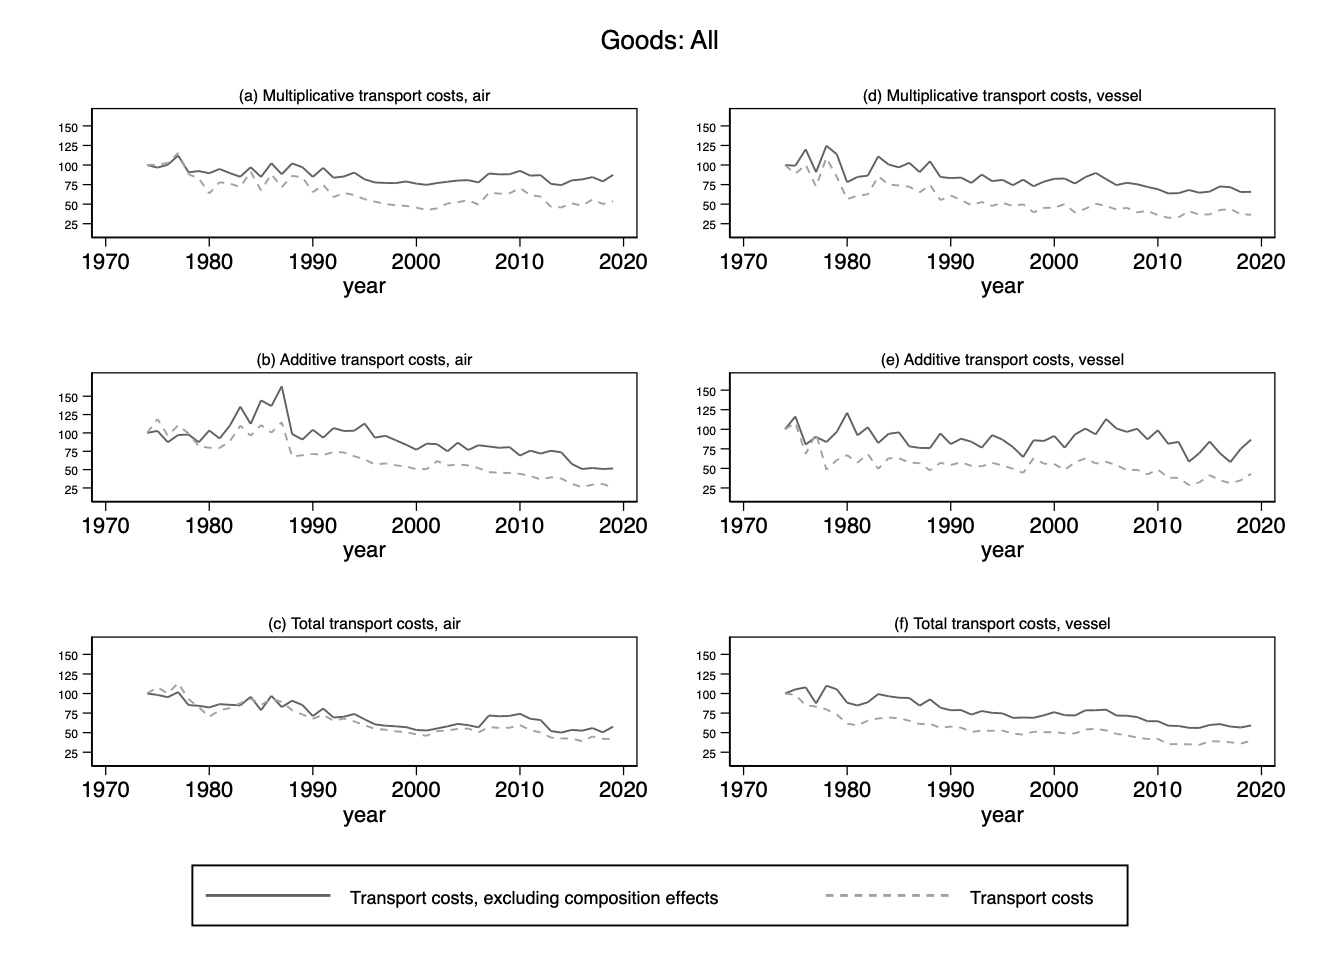
\includegraphics[height=8cm]
{graph_composition_all_np.jpg}
\end{center}
\end{figure}

The comparison of Figure \ref{fig:compeffects_robustness} (applying \citealp{hummels2007}'s weighting scheme) and Figure \ref{fig:totalTC_compeffects_excl} (applying our weighting scheme) prompts two comments.
First, differences do show up, in particular for the multiplicative component of air transport.
This suggests that the weighting scheme is not innocuous in the time trend decomposition exercise.
However, Figure \ref{fig:compeffects_robustness} also shows that the composition effects have contributed to strengthen the decrease in the ``ceteris paribus'' transport costs in air transport (in Figure \ref{fig:compeffects_robustness}, panel (a), overall transport costs have decreased more than the fitted component), in accordance with the conclusions drawn from Figure \ref{fig:totalTC_compeffects_excl}, rather than partly offsetting this decline, as argued by \cite{hummels2007}.
This confirms that it is the functional form and precisely the modeling of the additive component, rather than the weighting scheme, that is key in understanding the underlying determinants of the overall transport costs time trends, as pointed out in Section \ref{sec:results_trends}.


\section{More on the model \label{app:theoretical_model}}

\subsection{The model in the general case}

In this section, we provide more details on the model's solving in the general case, i.e. without specifying any functional form for the distribution of firm productivity.

\subsubsection{Aggregation: Price indices}


Following \cite{melitz}, and decomposing the set of available varieties into $\Omega_d$, $\Omega_x$ the set of varieties respectively produced at Home and imported, one can rewrite the price index (\ref{eq:CPI}) as:
\begin{eqnarray*}
P &=& \left[\int_{\omega \in \Omega_d} p_d^{1-\sigma}(\omega)d\omega + \int_{\omega \in \Omega_x} p_x^{1-\sigma}(\omega)d\omega  \right]^{\frac{1}{1-\sigma}} \\
&=& \left[\int_{0}^\infty p_d^{1-\sigma}(\varphi)M\mu(\varphi)d\varphi + \int_{0}^\infty p_x^{1-\sigma}(\varphi)M_x \mu_x(\varphi)d\varphi  \right]^{\frac{1}{1-\sigma}}
\end{eqnarray*}
Making use of Equation (\ref{eq:muofphi}), the price index reads as:
\begin{eqnarray*}
P &=& \left[\frac{M}{1-G(\varphi^\ast)}\int_{\varphi^\ast}^\infty p_d^{1-\sigma}(\varphi)g(\varphi)d\varphi + \frac{M_x}{1-G(\varphi_x^\ast)}\int_{\varphi^\ast_x}^\infty p_x^{1-\sigma}(\varphi)g(\varphi)d\varphi  \right]^{\frac{1}{1-\sigma}} \\
\text{with}&& \left\{
\begin{array}{lll}
p_d(\varphi)&=& \frac{\sigma}{\sigma-1} \frac{1}{\varphi}\\
p_x(\varphi)&=& \frac{\sigma}{\sigma-1} \left[\frac{\tau}{\varphi} +t\right]
\end{array}
\right.
\end{eqnarray*}
Accordingly, the price index can be rewritten as:
$$P = \left(\frac{\sigma}{\sigma-1}\right)\left[\frac{M}{1-G(\varphi^\ast)}\int_{\phi^\ast}^\infty \phi^{\sigma-1}g(\varphi)d\varphi + \frac{M_x}{1-G(\varphi_x^\ast)}\int_{\varphi^\ast_x}^\infty \left[\varphi \left(\frac{\tau}{\tau+t \varphi}  \right)  \right]^{\sigma-1}g(\varphi)d\varphi  \right]^{\frac{1}{1-\sigma}}$$


Similarly as in the closed-economy case (\cite{melitz}), let us define $\widetilde{\varphi}(\varphi^\ast)$ and $\widetilde{\varphi}_x(\varphi_x^\ast)$ as the weighted average of productivities of the domestic firms, on the domestic market and the export market respectively:\footnote{In the symmetric two-country model, $\widetilde{\varphi}_x(\varphi_x^\ast)$ also corresponds to the weighted average of productivities of foreign exporters at Home, e.g. associated with the imported varieties.}

\begin{eqnarray}
\widetilde{\varphi} &=& \left[\frac{1}{1-G(\varphi^\ast)}\int_{\varphi^\ast}^\infty \phi^{\sigma-1}g(\varphi)d\varphi   \right]^{\frac{1}{\sigma-1}} \label{eq:def_phitilde}\\
\widetilde{\varphi}_x &=& \left[\frac{1}{1-G(\varphi_x^\ast)}\int_{\varphi^\ast}^\infty \left[\varphi\left(\frac{\tau}{\tau+t \varphi}  \right) \right]^{\sigma-1}g(\varphi)d\varphi   \right]^{\frac{1}{\sigma-1}} \label{eq:def_phitildex}
\end{eqnarray}

\subsubsection{Solving the general equilibrium}

Following \cite{melitz} and the subsequent literature, denoting $M_e$ the mass of prospective entrants and $\rho_e$ the probability of successful entry (equal to $1-G(\varphi^\ast)$), considering only steady-state equilibrium needs to verify the entry-exit flow equilibrium condition:
$$\rho_e M_e = \delta M$$.

Given the wage normalization, total revenue in each country should be such that: $E = L_p+\Pi$, with $L_p$ the number of workers of the productive sector and $\Pi$ total profits. Labor market equilibrium further requires: $L = L_p+ L_e$ with $L_e = f_eM_e$ as sunk entry costs are paid in terms of labor. Combining this with the free-entry condition (\ref{eq:FEC}), we obtain that $\Pi = L_e$: Total profits in the productive sector are used to pay the entry sunk costs. Making use of this, we obtain that aggregate income in each country is equal to its labor endowment: $E =L$.

Further, total revenue can de expressed as the product of the average sales and the mass of active producers, according to: $E = M\bar{r}$, with $\bar{r}$ average sales. Similarly as for profits, it can be expressed as the sum of average sales on each local and foreign market:
$$\bar{r} = r_d(\widetilde{\varphi}(\varphi^\ast))+ \rho_x r_d(\widetilde{\varphi}_x(\varphi_x^\ast))$$
\noindent with the (conditional) probability of export $\rho_x = \frac{1-G(\varphi^\ast_x)}{1-G(\varphi^\ast)}$ and average sales on each market which can be shown to be:
\begin{eqnarray*}
\bar{r}_d &=& \left(\frac{\widetilde{\varphi}^\ast}{\varphi^\ast}\right)^{\sigma-1} \sigma f \\
\bar{r}_x &=& \left(\frac{\widetilde{\varphi}_x^\ast}{\varphi_x^\ast}\right)^{\sigma-1}\left(\frac{\tau+ t \varphi^\ast_x}{\tau+ t \widetilde{\varphi}^\ast_x}\right)^{\sigma-1} \sigma f_x
\end{eqnarray*}

Given selection on the export market, the mass of domestic exporters depends on that of domestic active firms according to: $M_x = \rho_x M$. In the symmetric equilibrium, the total mass of available varieties is then: $M_T= M+M_x = (1+\rho_x)M$.

\subsubsection{Summary}

Equations (\ref{eq:def_phitilde}), (\ref{eq:def_phitildex}), (\ref{eq:ZCP}), (\ref{eq:link_thresholds}) and (\ref{eq:FEC}) determine a system of interdependent equations in five endogenous variables $\left\{\bar{\pi}, \widetilde{\varphi}, \widetilde{\varphi}_x, \varphi^\ast, \varphi^\ast_x \right\}$. We can deduce the equilibrium values of the remaining set of variables $\left\{P, M_T, M, M_x, \widetilde{\varphi}_T, \bar{r} \right\}$ by recursively solving the following set of equations:

\begin{eqnarray*}
% \nonumber % Remove numbering (before each equation)
 \bar{r}&=& \left(\frac{\widetilde{\varphi}^\ast}{\varphi^\ast}\right)^{\sigma-1} \sigma f + \frac{1-G(\varphi^\ast_x)}{1-G(\varphi^\ast)}\left(\frac{\widetilde{\varphi}_x^\ast}{\varphi_x^\ast}\right)^{\sigma-1}\left(\frac{\tau+ t \varphi^\ast_x}{\tau+ t \widetilde{\varphi}^\ast_x}\right)^{\sigma-1} \sigma f_x \\
 M &=& \frac{L}{\bar{r}} \\
M_x &=& \frac{1-G(\varphi^\ast_x)}{1-G(\varphi^\ast)} M \\
M_T &=& \left(1+ \frac{1-G(\varphi^\ast_x)}{1-G(\varphi^\ast)} \right)M \\
\widetilde{\varphi}_T &=& \widetilde{\varphi}_T \equiv \left[\frac{1}{M_T}\left(M\widetilde{\varphi}^{\sigma-1} + M_x \left( \frac{\widetilde{\varphi}_x}{\tau} \right)^{\sigma-1} \right)  \right]^{\frac{1}{1-\sigma}} \\
P &=& M_T^{\frac{1}{1-\sigma}} \frac{\rho}{\widetilde{\varphi}_T}
\end{eqnarray*}


\subsection{With a Pareto distribution}


As in most of the related literature (\cite{Irrazabal_2015}, \cite{melitz-redding-Handbk-IT-2014}, \cite{ghironi}), we adopt a Pareto distribution for firm productivity heterogeneity, with the density and the cumulative functions respectively written as:
\begin{eqnarray*}
g(\varphi) &=& k\varphi_{\text{min}}^k \varphi^{-(k+1)}\\
G(\varphi) &=& 1 -\left( \frac{\varphi_{\text{min}}}{\varphi} \right)^k
\end{eqnarray*}

With the Pareto distribution, the system of Equations (\ref{eq:def_phitilde}), (\ref{eq:def_phitildex}), (\ref{eq:ZCP}), (\ref{eq:link_thresholds}) and (\ref{eq:FEC}) can be rewritten as a system of four equations in four endogenous variables: $\left\{\bar{\pi}, g(\varphi_x^\ast),\varphi_x^\ast, \varphi^\ast  \right\}$ as given by:

\begin{eqnarray}
\bar{\pi}&=& \frac{\sigma-1}{k-(\sigma-1)}f + \left(\varphi^\ast \right)^k f_x\left[k\left(\frac{\tau}{\varphi_x^\ast}+t  \right)^{\sigma-1}\left[  1+(k(\varphi_x^\ast)^k g(\varphi_x^\ast))^{\frac{1}{\sigma-1}}\right]^{1-\sigma}  - \left( \varphi_x^\ast \right)^{-k} \right] \label{eq:systemPareto_1}\\
g(\varphi_x^\ast)&=&\int_{\varphi_x^\ast}^\infty \varphi^{\sigma-1-(k+1)}(\tau +t\varphi)^{1-\sigma}d\varphi \label{eq:systemPareto_2} \\
\frac{\varphi_x^\ast}{\tau+ t\varphi_x^\ast}&=&\varphi^\ast \left[ \frac{f}{f_x} \right]^{\frac{1}{1-\sigma}} \label{eq:systemPareto_3}\\
\bar{\pi}&=& \delta f_e \left( \frac{\varphi^\ast}{\varphi_{\text{min}}} \right)^k \label{eq:systemPareto_4}
\end{eqnarray}

Notice that, in the absence of additive costs ($t=0$), Equation (\ref{eq:systemPareto_2}) rewrites as:
$$g(\varphi_x^\ast) = \tau^{1-\sigma}\left[ \frac{(\varphi_x^\ast)^{-(k-(\sigma-1))}}{k-(\sigma-1)}\right]$$
The system of Equations (\ref{eq:systemPareto_1})-((\ref{eq:systemPareto_4}) thus simplifies to be solved recursively with a full analytical solution. This is no longer the case in the presence of additive costs, and we have to rely on the model's simulations to obtain the general equilibrium of the model for a given calibration of the deep parameters.


\end{document} 